% !TeX program = xelatex
\documentclass[a4paper,12pt]{article}

% ===== 1. KHỔ GIẤY, LỀ TRANG, FONT =====
\usepackage[left=3cm,right=2cm,top=2cm,bottom=2cm,footskip=1cm]{geometry}
\usepackage{fontspec}

\IfFontExistsTF{Times New Roman}{
  \setmainfont{Times New Roman}
}{
  \IfFileExists{fonts/times.ttf}{
    \setmainfont{times.ttf}[
      Path=fonts/,
      BoldFont=timesbd.ttf,
      ItalicFont=timesi.ttf,
      BoldItalicFont=timesbi.ttf]
  }{
    \IfFontExistsTF{TeX Gyre Termes}{
      \setmainfont{TeX Gyre Termes}
      \PackageWarningNoLine{MauBaoCao}{Times New Roman unavailable; using TeX Gyre Termes}
    }{
      \setmainfont{DejaVu Serif}
      \PackageWarningNoLine{MauBaoCao}{Times New Roman unavailable; using DejaVu Serif}
    }
  }
}
\usepackage{indentfirst}
\usepackage{microtype}
\usepackage{colortbl}
\usepackage{needspace}
\usepackage{graphicx}
\usepackage{float}
\usepackage{tikz}
\usepackage{amsmath,amssymb}
\usepackage{array,tabularx,booktabs,longtable}
\usepackage{enumitem}
\usepackage{titlesec}
\usepackage{tocloft}
\usepackage{caption}
\usepackage{xurl}
\usepackage[unicode,hidelinks]{hyperref}
\urlstyle{same}

\renewcommand{\normalsize}{\fontsize{13}{19.5}\selectfont}
\AtBeginDocument{\normalsize}
\setlength{\parindent}{0.5cm}
\setlength{\parskip}{4pt}
\setlength{\emergencystretch}{3em}
\hyphenpenalty=10000
\exhyphenpenalty=10000
\raggedbottom
\setlist{topsep=4pt,itemsep=2pt,parsep=0pt,leftmargin=*}

% ===== 2. BA CẤP TIÊU ĐỀ: 1 / 1.1 / 1.1.1 =====
\setcounter{secnumdepth}{3}
\setcounter{tocdepth}{3}
\renewcommand{\thesection}{\arabic{section}}
\renewcommand{\thesubsection}{\thesection.\arabic{subsection}}
\renewcommand{\thesubsubsection}{\thesubsection.\arabic{subsubsection}}
\titleformat{\section}[hang]
  {\normalfont\fontsize{16}{20}\selectfont\bfseries}
  {\thesection.}{0.6em}{}
\titleformat{\subsection}[hang]
  {\normalfont\fontsize{14}{18}\selectfont\bfseries}
  {\thesubsection}{0.6em}{}
\titleformat{\subsubsection}[hang]
  {\normalfont\fontsize{13}{17}\selectfont\bfseries}
  {\thesubsubsection}{0.6em}{}
\titlespacing*{\section}{0pt}{16pt}{8pt}
\titlespacing*{\subsection}{0pt}{12pt}{6pt}
\titlespacing*{\subsubsection}{0pt}{8pt}{4pt}

% ===== 3. MỤC LỤC VÀ SỐ TRANG =====
\renewcommand{\contentsname}{MỤC LỤC}
\renewcommand{\listfigurename}{Danh sách hình vẽ}
\renewcommand{\listtablename}{Danh sách bảng}
\renewcommand{\cftloftitlefont}{\fontsize{16}{20}\selectfont\bfseries}
\renewcommand{\cftlottitlefont}{\fontsize{16}{20}\selectfont\bfseries}
\setlength{\cftbeforeloftitleskip}{0pt}\setlength{\cftafterloftitleskip}{14pt}
\setlength{\cftbeforelottitleskip}{0pt}\setlength{\cftafterlottitleskip}{14pt}
\renewcommand{\cftfigpresnum}{Hình }\renewcommand{\cfttabpresnum}{Bảng }
\renewcommand{\cftfigaftersnum}{.}\renewcommand{\cfttabaftersnum}{.}
\cftsetindents{figure}{0em}{5em}\cftsetindents{table}{0em}{5.2em}
\setlength{\cftbeforefigskip}{0pt}\setlength{\cftbeforetabskip}{0pt}
\renewcommand{\refname}{Tài liệu tham khảo}
\renewcommand{\cfttoctitlefont}{\fontsize{16}{20}\selectfont\bfseries}
\setlength{\cftbeforetoctitleskip}{0pt}
\setlength{\cftaftertoctitleskip}{18pt}
\renewcommand{\cftsecfont}{\normalfont\bfseries}
\renewcommand{\cftsecpagefont}{\normalfont\bfseries}
\renewcommand{\cftsubsecfont}{\normalfont}
\renewcommand{\cftsubsubsecfont}{\normalfont}
\renewcommand{\cftsecleader}{\cftdotfill{\cftdotsep}}
\cftsetindents{section}{0em}{2em}
\cftsetindents{subsection}{2em}{3em}
\cftsetindents{subsubsection}{5em}{4em}
\setlength{\cftbeforesecskip}{6pt}
\makeatletter
\def\ps@plain{%
  \let\@oddhead\@empty\let\@evenhead\@empty
  \def\@oddfoot{\hfil{\normalfont\fontsize{11}{13}\selectfont\thepage}\hfil}%
  \let\@evenfoot\@oddfoot}
\makeatother
\pagestyle{plain}

% ===== 4. BẢNG, HÌNH, CHÚ THÍCH =====
\counterwithin{figure}{section}
\counterwithin{table}{section}
\renewcommand{\topfraction}{0.9}\renewcommand{\bottomfraction}{0.8}
\renewcommand{\textfraction}{0.08}\renewcommand{\floatpagefraction}{0.75}
\setcounter{topnumber}{3}\setcounter{totalnumber}{4}
\renewcommand{\tablename}{Bảng}
\renewcommand{\figurename}{Hình}
\DeclareCaptionFont{reportcaption}{\fontsize{12}{15}\selectfont}
\captionsetup{font=reportcaption,labelfont=bf,labelsep=period,
  justification=centering,skip=6pt}
\newcommand{\bangfont}{\fontsize{11}{14}\selectfont\setlength{\tabcolsep}{4.2pt}\renewcommand{\arraystretch}{1.2}}
\newcommand{\bangnho}{\fontsize{10}{12.5}\selectfont\setlength{\tabcolsep}{4.2pt}\renewcommand{\arraystretch}{1.2}}
\newcolumntype{L}[1]{>{\raggedright\arraybackslash}m{#1}}
\newcolumntype{C}[1]{>{\centering\arraybackslash}m{#1}}
\newcommand{\dongdau}{\rowcolor[gray]{0.92}}
\newcommand{\code}[1]{\texttt{#1}}

% ===== 5. THÔNG TIN TRANG BÌA =====
\newcommand{\DonViChuQuan}{ĐẠI HỌC QUỐC GIA HÀ NỘI}
\newcommand{\TenTruong}{TRƯỜNG ĐẠI HỌC CÔNG NGHỆ}
\newcommand{\LoaiBaoCao}{BÁO CÁO DỰ ÁN}
\newcommand{\TenMonHoc}{VẤN ĐỀ HIỆN ĐẠI TRONG CÔNG NGHỆ THÔNG TIN}
\newcommand{\TenDeTai}{NỀN TẢNG ẨN DANH HOÁ ẢNH VÀ VIDEO\\REDACTFUNNEL}
\newcommand{\GiangVien}{[Họ tên giảng viên]}
\newcommand{\DiaDiemThoiGian}{Hà Nội, tháng 11 năm 2026}
\hypersetup{pdftitle={BÁO CÁO DỰ ÁN - REDACTFUNNEL},pdfauthor={Nhóm sinh viên VNU-UET}}

\begin{document}

% ===== 6. TRANG BÌA CHUẨN UET =====
\begin{titlepage}
\thispagestyle{empty}
\begin{tikzpicture}[remember picture,overlay]
  \draw[line width=2pt]
    ([xshift=3cm,yshift=-2cm]current page.north west)
    rectangle ([xshift=-2cm,yshift=2cm]current page.south east);
  \draw[line width=0.5pt]
    ([xshift=3.12cm,yshift=-2.12cm]current page.north west)
    rectangle ([xshift=-2.12cm,yshift=2.12cm]current page.south east);
\end{tikzpicture}\par
\centering
\setlength{\parindent}{0pt}
\setlength{\parskip}{0pt}
\vspace*{0.8cm}
{\fontsize{14}{18}\selectfont\bfseries\DonViChuQuan\par}
\vspace{0.15cm}
{\fontsize{15}{20}\selectfont\bfseries\TenTruong\par}
\vspace{0.25cm}
\rule{5cm}{0.4pt}\par
\vspace{0.5cm}

\IfFileExists{logo.png}{
  
\includegraphics[width=3.8cm,height=3.8cm,keepaspectratio]{logo.png}
}{
  \IfFileExists{figures/logo.png}{
    
\includegraphics[width=3.8cm,height=3.8cm,keepaspectratio]{figures/logo.png}
  }{
    \fbox{\parbox[c][3.4cm][c]{3.4cm}{\centering
      \fontsize{11}{14}\selectfont LOGO TRƯỜNG}}
  }
}\par
\vspace{0.7cm}
{\fontsize{22}{27}\selectfont\bfseries\LoaiBaoCao\par}
\vspace{0.35cm}
\begin{minipage}{0.9\textwidth}\centering
  {\fontsize{15}{20}\selectfont\bfseries MÔN HỌC: \TenMonHoc\par}
\end{minipage}\par
\vspace{0.6cm}
{\fontsize{13}{17}\selectfont\bfseries ĐỀ TÀI\par}
\vspace{0.12cm}
\begin{minipage}{0.9\textwidth}\centering
  {\fontsize{16}{21}\selectfont\bfseries\TenDeTai\par}
\end{minipage}\par
\vspace{0.65cm}
{\fontsize{13}{19.5}\selectfont
\renewcommand{\arraystretch}{1.1}
\begin{tabular}{@{}>{\raggedright\arraybackslash\bfseries}p{5.2cm}>{\raggedright\arraybackslash}p{8cm}@{}}
  Giảng viên hướng dẫn: & \GiangVien\\
  Sinh viên thực hiện:  & Phạm Tất Đạt -- 24020063 \textbf{(Trưởng nhóm)}\\
                        & Nguyễn Đức Huy -- 24020162\\
                        & Nguyễn Đức Huy -- 22021186
\end{tabular}\par}
\vfill
{\fontsize{13}{17}\selectfont\bfseries\DiaDiemThoiGian\par}
\vspace*{0.5cm}
\end{titlepage}

% ===== 7. LỜI CAM ĐOAN & TÓM TẮT & PHÂN CÔNG (ROMAN NUMBERING) =====
\pagenumbering{roman}
\section*{Lời cam đoan}
\addcontentsline{toc}{section}{Lời cam đoan}
Chúng em xin cam đoan đề tài ``RedactFunnel: Nền tảng ẩn danh hoá ảnh và video'' là sản phẩm do nhóm tự thực hiện trong quá trình học tập và làm dự án. Mã nguồn, cấu hình triển khai và các mô hình được huấn luyện trình bày trong báo cáo đều do nhóm xây dựng. Số liệu thực nghiệm được đo trên hạ tầng của nhóm; file kết quả và script để chạy lại được lưu trong kho mã nguồn của dự án.

Đề tài có sử dụng thư viện và mô hình của bên thứ ba như Ultralytics YOLO, ArcFace, YuNet, RapidOCR và ByteTrack. Ảnh dùng để huấn luyện và đánh giá lấy từ các bộ dữ liệu công khai (WIDER FACE, LFW và một số bộ dữ liệu biển số xe Việt Nam); video dùng để đánh giá là một số video được đăng công khai trên mạng xã hội. Các nguồn này được ghi rõ trong báo cáo và ở phần Tài liệu tham khảo. Nhóm chỉ dùng chúng cho mục đích học tập và nghiên cứu, không đăng tải lại hay phân phối lại ảnh, video gốc. Các khung hình trích từ những video này trong báo cáo đều đã được che khuôn mặt và biển số.

Chúng em xin chịu trách nhiệm về tính trung thực của nội dung báo cáo này.

\clearpage
\section*{Tóm tắt}
\addcontentsline{toc}{section}{Tóm tắt}
Ảnh và video đăng lên mạng xã hội, ảnh chụp sự kiện hay video từ camera hành trình thường có khuôn mặt người qua đường và biển số xe của những người không liên quan. Từ ngày 01/01/2026, Luật Bảo vệ dữ liệu cá nhân số 91/2025/QH15 có hiệu lực, nên việc công khai các thông tin này cần được cân nhắc kỹ hơn. Che thủ công bằng phần mềm chỉnh sửa thì tốn nhiều thời gian. Các dịch vụ AI trên cloud đòi hỏi trả phí, niềm tin vào dịch vụ hoặc yêu cầu tự chuẩn bị pipeline xử lý.

Đề tài xây dựng RedactFunnel, một nền tảng web mã nguồn mở có thể tự triển khai, dùng để tự động phát hiện và che khuôn mặt, biển số xe trong ảnh và video ngắn. Người dùng tải lên một bộ ảnh hoặc video, chọn đối tượng cần che và kiểu che, có thể thêm ảnh chân dung hay biển số cần giữ nguyên. Sau khi xử lý, người dùng xem kết quả trước và sau khi che, sửa thủ công vùng che nếu cần, rồi tải kết quả về cùng một báo cáo liệt kê những chỗ nên kiểm tra lại.

Hệ thống được thiết kế theo kiến trúc hướng sự kiện. Phần web chỉ nhận file, lưu lên MinIO và đưa job vào hàng đợi NATS JetStream. Worker AI viết bằng Python chạy tách riêng thành hai nhóm cho ảnh và cho video; KEDA tăng giảm số worker theo số job đang chờ và đưa về 0 khi không có việc. Toàn bộ hệ thống chạy trên một cụm Kubernetes và được thử nghiệm trên hai mãy chủ: một máy chủ CPU 4 luồng, 12 GB RAM, không có GPU; và một máy chủ CPU 16 luồng, 16GB RAM, có GPU.

Về mô hình, nhóm fine-tune YOLO26 trên WIDER FACE và dữ liệu biển số Việt Nam với ảnh đầu vào 1280 px, sau đó huấn luyện thêm trên 468 khung hình camera hành trình, giúp số biển số đọc được bị bỏ sót trên video giảm từ 2 đến 4 lần. Trên bộ kiểm thử 3.726 ảnh không dùng khi huấn luyện, ở cùng độ chính xác (precision) với công cụ mã nguồn mở deface, mô hình nhỏ YOLO26n che được 80,3\% số khuôn mặt và mô hình lớn YOLO26s che được 82,8\%, còn deface che được 72,3\% và không phát hiện biển số. Whitelist khuôn mặt dùng ArcFace kết hợp căn chỉnh bằng YuNet: trên bộ LFW, hệ thống giữ đúng chủ thể trong khoảng 84\% trường hợp khi có một ảnh mẫu và 96\% khi có ba ảnh mẫu, còn người lạ chỉ bị giữ nhầm khoảng 3 lần trên 1 triệu lần so sánh. Phần đọc biển số dùng RapidOCR, đọc riêng từng nửa với biển hai dòng, đạt 88,6\% trên 536 biển xe máy và ô tô. Video được xử lý bằng ByteTrack và FFmpeg, giữ nguyên âm thanh gốc.

Với mô hình YOLO26n ở 1280 px và số worker tự co giãn từ 0 lên 3, hệ thống xử lý khoảng 1.470 ảnh mỗi phút trên máy có GPU và khoảng 84 ảnh mỗi phút trên máy chỉ có CPU. Trong các lần đo không có job nào bị mất. Những mục tiêu chưa đạt, gồm độ chính xác với khuôn mặt rất nhỏ và biển số bị che một phần trong video, được phân tích ở Chương 5.

\clearpage
\section*{Phân chia công việc và mức độ đóng góp}
\renewcommand{\thetable}{P.\arabic{table}}
\addcontentsline{toc}{section}{Phân chia công việc và mức độ đóng góp}
{\small\itshape\noindent\textbf{Ghi chú biên soạn:} Nội dung: Nêu rõ phần việc và mức đóng góp của từng thành viên. Mỗi người phụ trách trọn một trong ba khối web/, engine/, infra/ (docs/phân-công-và-guideline.md), các phần chéo ghi rõ người làm. Gợi ý lấy từ chủ sở hữu từng mục trong web/docs/plan.md, engine/docs/plan.md, docs/milestones.md và lịch sử git; nhóm thống nhất lại tỉ lệ \% trước khi nộp.  Nguồn: docs/phân-công-và-guideline.md, docs/milestones.md, web/docs/plan.md\par\vspace{8pt}}

\needspace{9\baselineskip}
{\bangfont
\begin{longtable}{|>{\raggedright\arraybackslash\bfseries}p{3.17cm}|>{\raggedright\arraybackslash}p{3.47cm}|>{\raggedright\arraybackslash}p{8.42cm}|}
\caption{Phân chia công việc và mức độ đóng góp của các thành viên}\label{tab:p1}\\
\hline
\dongdau \textbf{Thành viên} & \textbf{Vai trò} & \textbf{Công việc cụ thể đã thực hiện} \\
\hline
\endfirsthead
\multicolumn{3}{c}{\textbf{Bảng P.1.} Phân chia công việc và mức độ đóng góp (tiếp theo)}\\[2pt]
\hline
\dongdau \textbf{Thành viên} & \textbf{Vai trò} & \textbf{Công việc cụ thể đã thực hiện} \\
\hline
\endhead
\endfoot
\endlastfoot
Phạm Tất Đạt & Trưởng nhóm, vận hành hạ tầng, benchmark, hỗ trợ Web và Engine & 
\begin{itemize}[leftmargin=*,nosep]
  \item Thiết kế kiến trúc, lựa chọn công nghệ cho hệ thống
  \item Tạo Kubernetes manifest và script triển khai hạ tầng trên môi trường lab, truy cập qua Cloudflare Tunnel
  \item Tạo file docker-compose phục vụ cho quá trình phát triển và việc vận hành không cần đến cụm Kubernetes
  \item Thiết kế và xây dựng luồng upload, truy cập ảnh đối với MinIO cùng các cấu hình về thời gian lưu trữ, độ lớn file, rate limit
  \item Đánh nhãn, thu thập dữ liệu, huấn luyện AI model, chạy benchmark và tổng hợp kết quả. Hỗ trợ tối ưu luồng xử lý OCR biển số, xử lý nhận diện trên video.
  \item Kiểm thử chức năng, giao diện hệ thống
\end{itemize} \\ \hline
Nguyễn Đức Huy\newline(22021186) & Web (backend API, schema, frontend) & 
\begin{itemize}[leftmargin=*,nosep]
  \item Thiết kế và xây dựng REST API, schema PostgreSQL, xử lý schema validation và xác thực người dùng
  \item Xử lý logic nghiệp vụ quản lý batch, chạy batch, quản lý whitelist, tạo và cập nhật trạng thái job, tạo báo cáo
  \item Thiết kế và xây dựng giao diện quản lý thư viện, trình chiếu kết quả, kết nối giao diện với backend API
\end{itemize} \\ \hline
Nguyễn Đức Huy\newline(24020162) & Engine (OCR, detection) & 
\begin{itemize}[leftmargin=*,nosep]
  \item Thiết kế các job event trong NATS Jetstream, xây dựng luồng xử lý job, progress và lưu trữ kết quả cho AI worker
  \item Xây dựng và tối ưu luồng nhận diện và làm mờ trên ảnh và video, xử lý đọc OCR cho biển số
  \item Đánh nhãn, thu thập dữ liệu, huấn luyện AI model và benchmark
  \item Kiểm thử chức năng, giao diện hệ thống
\end{itemize} \\ \hline
\end{longtable}
}
\needspace{9\baselineskip}
{\bangfont
\begin{longtable}{|>{\raggedright\arraybackslash\bfseries}m{5.25cm}|>{\raggedright\arraybackslash}m{10.10cm}|}
\caption{Chia việc làm báo cáo}\label{tab:p2}\\
\hline
\dongdau \textbf{Thành viên} & \textbf{Công việc phụ trách} \\
\hline
\endfirsthead
\multicolumn{2}{c}{\textbf{Bảng P.2.} Chia việc làm báo cáo (tiếp theo)}\\[2pt]
\hline
\dongdau \textbf{Thành viên} & \textbf{Công việc phụ trách} \\
\hline
\endhead
\endfoot
\endlastfoot
Phạm Tất Đạt & 1, 2.2, 2.3.1, 3.1-3.3, 3.9, 5.4-5.7, 5.9, Kết luận \\ \hline
Nguyễn Đức Huy\newline(22021186) & 2.3.2, 3.4-3.7, 5.1, 5.2, 5.8 \\ \hline
Nguyễn Đức Huy\newline(24020162) & 2.1, 3.8, chương 4, 5.3 \\ \hline
\end{longtable}
}
\clearpage
{\setlength{\parskip}{0pt}\setlength{\cftbeforesecskip}{4pt}\fontsize{12.5}{17}\selectfont\tableofcontents}

\clearpage
\phantomsection
\addcontentsline{toc}{section}{\listfigurename}
{\setlength{\parskip}{0pt}\fontsize{12.5}{17.5}\selectfont\listoffigures}

\clearpage
\phantomsection
\addcontentsline{toc}{section}{\listtablename}
{\setlength{\parskip}{0pt}\fontsize{12.5}{17.5}\selectfont\listoftables}

\clearpage
\section*{Danh mục các từ viết tắt}
\addcontentsline{toc}{section}{Danh mục các từ viết tắt}

{\bangfont
\begin{longtable}{|>{\centering\arraybackslash}m{1.18cm}|>{\raggedright\arraybackslash\bfseries}m{2.46cm}|>{\raggedright\arraybackslash}m{5.41cm}|>{\raggedright\arraybackslash}m{5.70cm}|}
\hline
\dongdau \textbf{STT} & \textbf{Từ viết tắt} & \textbf{Tiếng Anh đầy đủ} & \textbf{Nghĩa tiếng Việt} \\
\hline
\endfirsthead
\multicolumn{4}{c}{{\bfseries Danh mục các từ viết tắt (tiếp theo)}}\\
\hline
\dongdau \textbf{STT} & \textbf{Từ viết tắt} & \textbf{Tiếng Anh đầy đủ} & \textbf{Nghĩa tiếng Việt} \\
\hline
\endhead
\endfoot
\endlastfoot
1 & AP & Average Precision & Độ chính xác trung bình \\ \hline
2 & mAP@50 & mean Average Precision at IoU 0.5 & AP trung bình các lớp tại ngưỡng IoU 0,5 \\ \hline
3 & IoU & Intersection over Union & Tỉ lệ giao trên hợp giữa hai hộp giới hạn \\ \hline
4 & YOLO & You Only Look Once & Họ mô hình phát hiện đối tượng một giai đoạn \\ \hline
5 & OCR & Optical Character Recognition & Nhận dạng ký tự quang học \\ \hline
6 & TAR & True Accept Rate & Tỉ lệ giữ đúng chủ thể trong whitelist \\ \hline
7 & FAR & False Accept Rate & Tỉ lệ giữ nhầm người lạ \\ \hline
8 & ONNX & Open Neural Network Exchange & Định dạng trao đổi mô hình học sâu \\ \hline
9 & CPU / GPU & Central / Graphics Processing Unit & Bộ xử lý trung tâm / bộ xử lý đồ hoạ \\ \hline
10 & API & Application Programming Interface & Giao diện lập trình ứng dụng \\ \hline
11 & REST & Representational State Transfer & Kiểu kiến trúc API dựa trên HTTP \\ \hline
12 & JWT & JSON Web Token & Chuỗi token xác thực có chữ ký \\ \hline
13 & ORM & Object Relational Mapping & Ánh xạ đối tượng sang cơ sở dữ liệu quan hệ \\ \hline
14 & S3 & Simple Storage Service & Chuẩn API lưu trữ đối tượng do Amazon đặt ra \\ \hline
15 & KEDA & Kubernetes Event-driven Autoscaling & Bộ co giãn Kubernetes theo sự kiện \\ \hline
16 & HPA & Horizontal Pod Autoscaler & Bộ co giãn số pod theo CPU/RAM của Kubernetes \\ \hline
17 & K8s & Kubernetes & Hệ thống điều phối container \\ \hline
18 & PVC & PersistentVolumeClaim & Yêu cầu cấp vùng lưu trữ bền vững trong Kubernetes \\ \hline
19 & CI/CD & Continuous Integration / Continuous Deployment & Tích hợp liên tục / triển khai liên tục \\ \hline
20 & UI & User Interface & Giao diện người dùng \\ \hline
21 & UC & Use Case & Ca sử dụng \\ \hline
22 & FPS & Frames Per Second & Số khung hình mỗi giây \\ \hline
23 & EXIF & Exchangeable Image File Format & Siêu dữ liệu đi kèm ảnh (máy chụp, vị trí GPS\dots{}) \\ \hline
24 & ROI & Region of Interest & Vùng ảnh cần xử lý \\ \hline
25 & GDPR & General Data Protection Regulation & Quy định chung về bảo vệ dữ liệu của Liên minh châu Âu \\ \hline
26 & BVDLCN &  & Bảo vệ dữ liệu cá nhân \\ \hline
\end{longtable}
}
\clearpage
\pagenumbering{arabic}
\renewcommand{\thetable}{\thesection.\arabic{table}}
\setcounter{page}{1}

\clearpage
\section{Đặt vấn đề}
\label{sec:ch1}


\subsection{Bối cảnh}

Việc quay phim, chụp ảnh và chia sẻ video ngắn trên TikTok, YouTube Shorts hay Facebook Reels giờ diễn ra hằng ngày. Camera hành trình trên ô tô, xe máy và camera giám sát ở khu dân cư, cửa hàng cũng ngày càng phổ biến. Kéo theo đó, khuôn mặt của người đi đường, người tham dự sự kiện và biển số của các phương tiện xung quanh bị ghi lại rồi lan truyền công khai, trong khi phần lớn những người này không liên quan đến nội dung và không biết mình đang bị quay.

Khuôn mặt và biển số xe có thể trở thành dữ liệu cá nhân khi chúng giúp xác định một người cụ thể. Ở Việt Nam, Luật Bảo vệ dữ liệu cá nhân số 91/2025/QH15 và Nghị định 356/2025/NĐ-CP có hiệu lực từ ngày 01/01/2026 đặt ra khung pháp lý cho việc thu thập, sử dụng và công khai loại dữ liệu này. Không phải mọi video quay ở nơi công cộng đều bị cấm, nhưng người đăng tải và tổ chức xử lý dữ liệu vẫn phải cân nhắc mục đích và căn cứ xử lý. Ở châu Âu, GDPR yêu cầu tối thiểu hoá dữ liệu, tức chỉ giữ lại những dữ liệu cá nhân thật sự cần cho mục đích xử lý; vi phạm có thể bị phạt tới 20 triệu euro hoặc 4\% doanh thu toàn cầu.

Vì vậy, nhu cầu che khuôn mặt và biển số trước khi công khai hay chuyển giao ảnh, video đã trở thành một bước xử lý bình thường với nhà báo, người làm nội dung, đơn vị vận hành camera và các nhóm phát triển AI cần dữ liệu hình ảnh.


\begin{figure}[htbp]
\centering
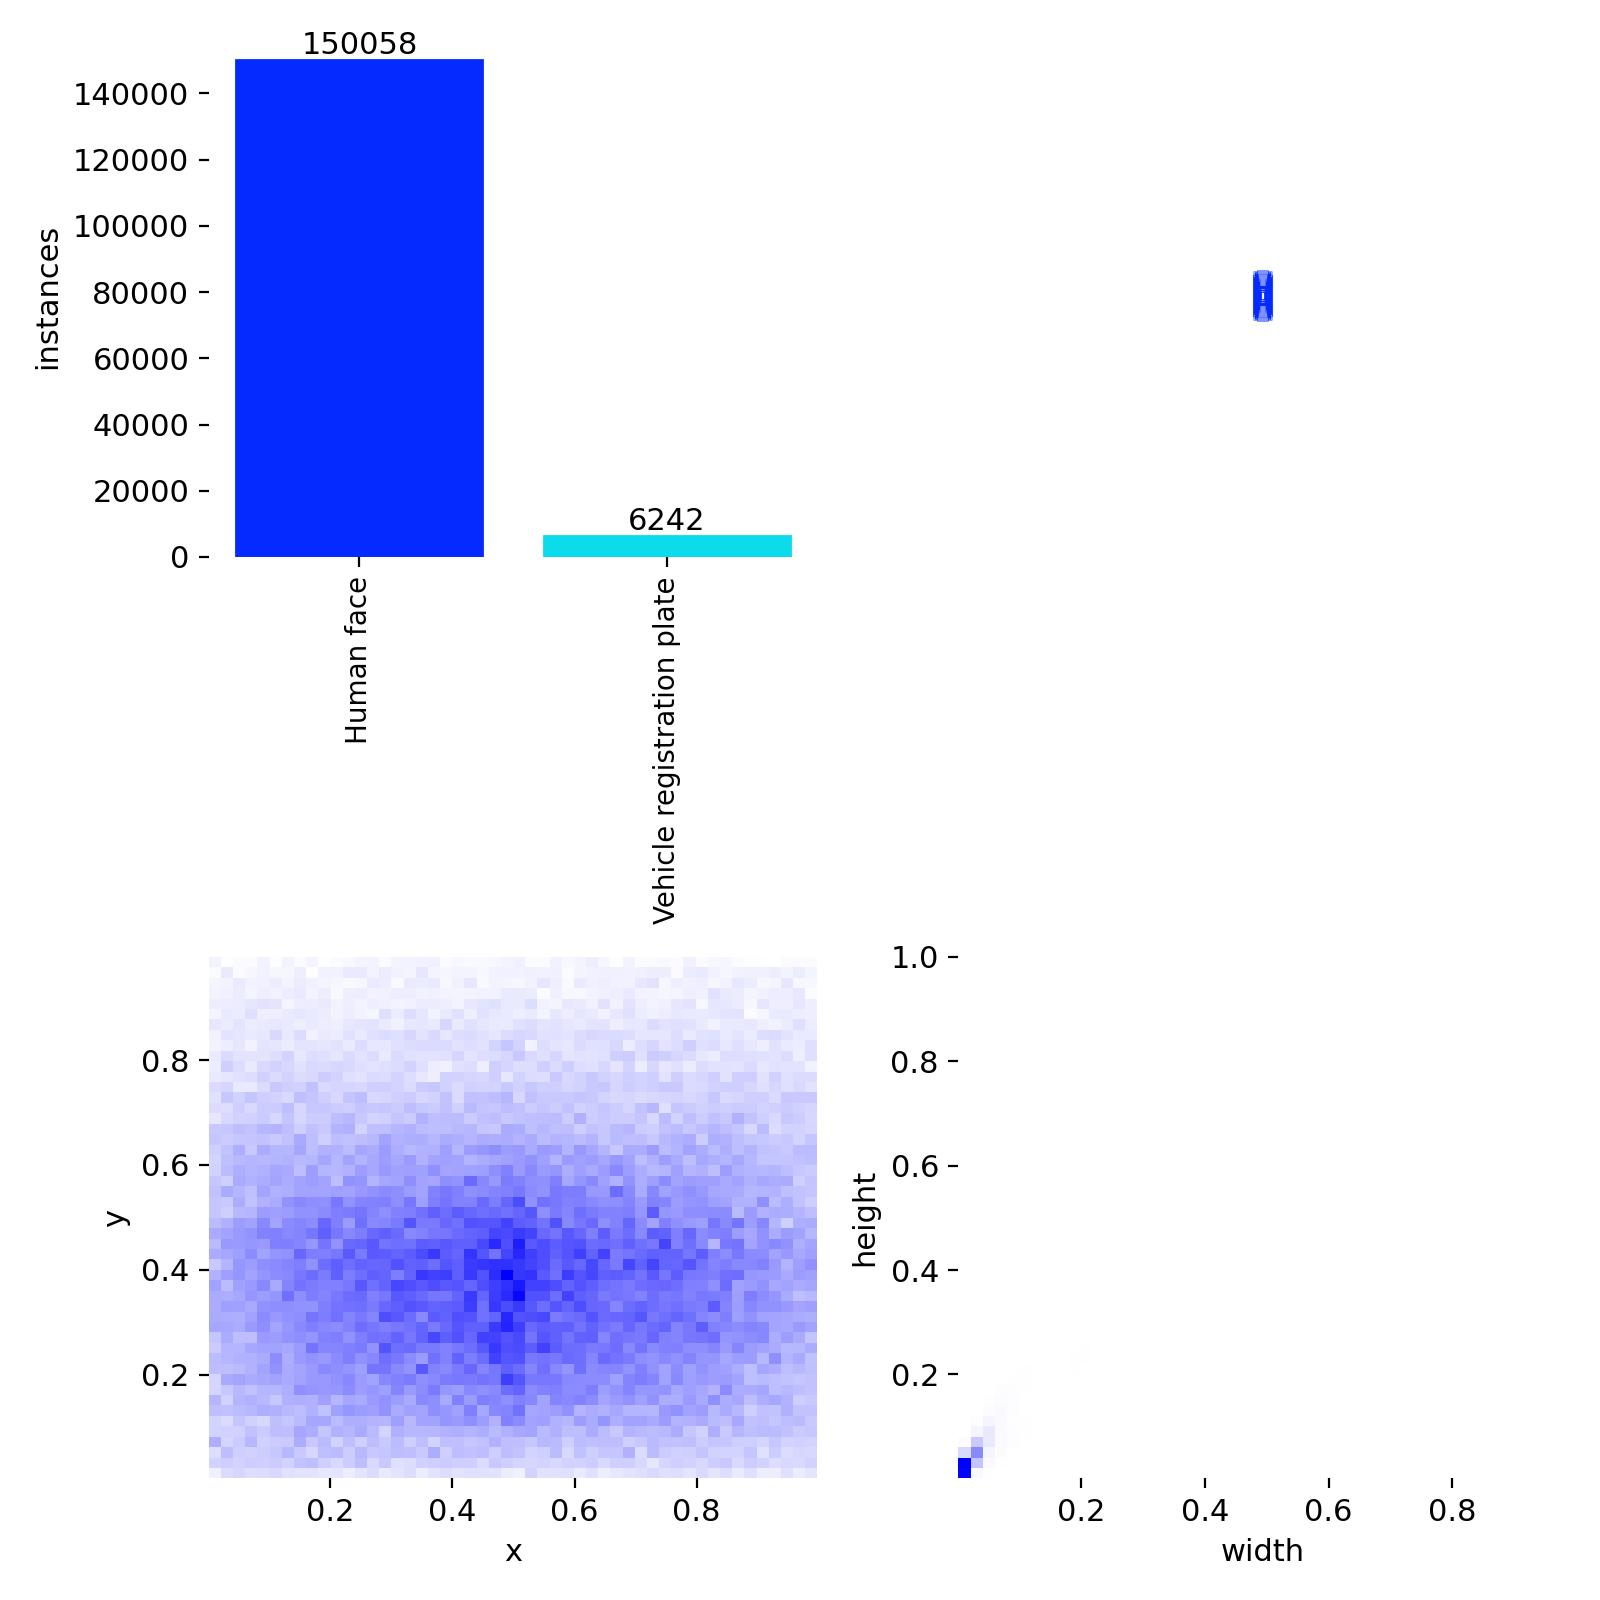
\includegraphics[width=0.88\textwidth]{figures/image3.jpeg}
\vspace{4pt}
{\small\itshape [HÌNH 1.1]Ảnh đường phố Việt Nam (người đi bộ, xe máy biển hai dòng), đặt cạnh bản đã che bằng RedactFunnel.Nguồn: infra/demo/sample.png hoặc khung hình (đã che) từ video đánh giá\par}
\caption{Ví dụ ảnh đường phố có khuôn mặt và biển số cần ẩn danh}
\label{fig:1-1}
\end{figure}


\subsection{Bài toán thực tế và nhu cầu người dùng}

Qua tìm hiểu, nhóm chia nhu cầu che thông tin nhận dạng thành bốn trường hợp chính:

\begin{itemize}[leftmargin=*,itemsep=2pt,parsep=0pt]
  \item Nhà sáng tạo nội dung, nhiếp ảnh gia và đội truyền thông phải xử lý nhiều ảnh, video trước khi xuất bản. Phát hiện và che tự động giúp giảm thời gian chỉnh sửa thủ công.
  \item Phóng sự, ảnh sự kiện và video từ camera hành trình cần một bản sao đã che để đăng công khai, trong khi bản gốc vẫn được giữ lại.
  \item Đơn vị vận hành camera, doanh nghiệp và nhóm phát triển AI cần chia sẻ dữ liệu hình ảnh cho bên thứ ba mà vẫn giảm lượng dữ liệu cá nhân bị chuyển giao.
  \item Người đăng video phản ánh giao thông hay sự cố ở nơi công cộng muốn giữ trọng tâm vào sự việc, không muốn làm lộ danh tính của những người khác trong khung hình.
\end{itemize}

Bài toán có một số đặc điểm khiến các công cụ chung chưa đáp ứng tốt. Thứ nhất, người dùng thường muốn giữ nguyên một số người hoặc phương tiện, chẳng hạn chính mình, người được phỏng vấn hay xe của mình, và chỉ che những người còn lại. Thứ hai, biển số xe máy Việt Nam có dạng vuông hai dòng, khác với biển một dòng mà đa số mô hình nước ngoài được huấn luyện. Thứ ba, ảnh đám đông và video camera hành trình có nhiều khuôn mặt, biển số rất nhỏ, dễ bị bỏ sót. Cuối cùng, với video, vùng che phải bám theo đối tượng qua các khung hình, không được nhấp nháy hay để lộ mặt trong vài khung khi mô hình phát hiện sót.

Trong bài toán này, bỏ sót một khuôn mặt hay biển số đồng nghĩa với việc lộ dữ liệu cá nhân, còn che nhầm một vùng không cần che chỉ làm ảnh xấu đi. Do đó nhóm ưu tiên độ phủ (recall) hơn độ chính xác (precision), và mọi trường hợp không chắc chắn đều được xử lý theo hướng che.


\subsection{Các phương pháp hiện có và hạn chế}


\subsubsection{Che thủ công bằng phần mềm chỉnh sửa}

Cách phổ biến nhất hiện nay là dùng Photoshop, Premiere, CapCut hoặc các ứng dụng chỉnh sửa trên điện thoại để vẽ vùng mờ lên từng ảnh, hoặc gắn hiệu ứng theo dõi chuyển động cho từng đối tượng trong video. Cách này cho kết quả đúng ý người làm, nhưng thời gian tăng theo số ảnh và số người xuất hiện. Với một thư mục vài trăm ảnh hay một video đông người, che thủ công gần như không khả thi, và người làm vẫn dễ bỏ sót những khuôn mặt, biển số nhỏ ở hậu cảnh.


\subsubsection{Dịch vụ AI thương mại trên cloud}

Các nền tảng như Amazon Rekognition hay Google Cloud Vision cung cấp API phát hiện khuôn mặt, chữ và đối tượng. Hạn chế là ảnh, video phải được gửi lên máy chủ của nhà cung cấp, thường đặt ở nước ngoài; chi phí tính theo số ảnh hoặc số phút video; phần lớn các API chỉ trả về toạ độ phát hiện đối tượng, việc che, quản lý danh sách người cần giữ nguyên và kiểm tra lại kết quả vẫn phải tự xây dựng. Ưu điểm của nhóm giải pháp này là độ chính xác tốt và không phải tự vận hành hạ tầng.

Một số dịch vụ chuyên về che dữ liệu trong video cũng đã có trên thị trường như SightHound Redactor. Ngoài việc cung cấp API trả phí, các dịch vụ này còn cung cấp khả năng tự vận hành server và tải ứng dụng desktop trên hạ tầng của người dùng, tuy nhiên chúng có các hạn chế: là một mô hình hộp đen để phục vụ cho kinh doanh theo subscription (2,500\$/năm - 3,500\$/năm), người dùng bị giới hạn số lượng tài khoản, không tuỳ chỉnh được về AI model, nhu cầu sử dụng, cách lưu trữ cũng như không thể kiểm tra mã nguồn. Ưu điểm của nhóm giải pháp này là một dịch vụ chuyên dùng để che có quy mô phát triển lớn, đáp ứng cả nhu cầu tự vận hành lẫn sử dụng API có sẵn


\subsubsection{Công cụ mã nguồn mở chạy cục bộ}

Một số công cụ mã nguồn mở đã giải quyết phần phát hiện và che. deface dùng mô hình CenterFace để làm mờ khuôn mặt trong ảnh và video, nhưng không xử lý biển số. EgoBlur của Meta có mô hình cho cả khuôn mặt và biển số, được huấn luyện cho dữ liệu camera đeo người. YuNet trong OpenCV là bộ phát hiện khuôn mặt rất nhẹ. Ngoài ra có nhiều dự án dùng YOLO và OCR cho biển số Việt Nam, chủ yếu phục vụ bài toán nhận dạng biển số ở bãi xe hoặc trạm thu phí.

Các công cụ này chạy được trên máy cá nhân và không phải gửi dữ liệu ra ngoài, nhưng chúng là công cụ dòng lệnh xử lý từng file trên một máy. Không công cụ nào có hàng đợi, giao diện xem lại kết quả, whitelist hay báo cáo những chỗ cần kiểm tra. Khi nhóm đo trên cùng bộ dữ liệu (Chương 4), deface che được 72,3\% số khuôn mặt và YuNet che được 73,7\% ở cùng độ chính xác với deface; EgoBlur chỉ che được 57,2\% dù đã hạ ngưỡng xuống mức thấp nhất. Với các dự án biển số Việt Nam, độ ổn định trên video thực tế, nơi biển nhỏ, nghiêng, rung hoặc bị che khuất, vẫn cần được kiểm thử thêm.

\needspace{13\baselineskip}
{\bangfont
\begin{longtable}{|>{\raggedright\arraybackslash\bfseries}m{2.81cm}|>{\raggedright\arraybackslash}m{2.81cm}|>{\raggedright\arraybackslash}m{2.81cm}|>{\raggedright\arraybackslash}m{2.81cm}|>{\raggedright\arraybackslash}m{3.21cm}|}
\caption{So sánh các phương pháp ẩn danh hoá hiện có}\label{tab:1-1}\\
\hline
\dongdau \textbf{Tiêu chí} & \textbf{Che thủ công} & \textbf{Dịch vụ AI thương mại} & \textbf{Công cụ mã nguồn mở} & \textbf{RedactFunnel} \\
\hline
\endfirsthead
\multicolumn{5}{c}{\textbf{Bảng 1.1.} So sánh các phương pháp ẩn danh hoá hiện có (tiếp theo)}\\[2pt]
\hline
\dongdau \textbf{Tiêu chí} & \textbf{Che thủ công} & \textbf{Dịch vụ AI thương mại} & \textbf{Công cụ mã nguồn mở} & \textbf{RedactFunnel} \\
\hline
\endhead
\endfoot
\endlastfoot
Tự động phát hiện & Không & Có, phần che phải tự làm & Có & Có \\ \hline
Xử lý hàng loạt, video & Làm từng ảnh, từng đoạn & Có API ảnh và video, có xử lý theo lô nhưng không tiết lộ cách triển khai & Chạy tuần tự trên một máy & Hàng đợi, worker tự co giãn \\ \hline
Biển số Việt Nam, hai dòng & Người làm tự chọn & Không tối ưu riêng & deface không có; EgoBlur yếu với biển nhỏ & Fine-tune trên dữ liệu Việt Nam, logic xử lý OCR \\ \hline
Giữ nguyên người, xe chỉ định & Người làm tự chọn & Phải tự tích hợp & Không có & Whitelist khuôn mặt và biển số \\ \hline
Dữ liệu ở lại hạ tầng riêng & Có & Tuỳ dịch vụ & Có & Có, tự triển khai \\ \hline
Chi phí & Công sức người làm & Theo lượt ảnh, phút video, subscription, API, máy chủ & Miễn phí & Miễn phí, cần máy chủ \\ \hline
Báo cáo, kiểm tra lại & Không & Tuỳ dịch vụ & Không & Báo cáo cần xem lại, sửa tay \\ \hline
\end{longtable}
}
\vspace{6pt}

{\small\itshape\noindent\textbf{Ghi chú biên soạn:} Nguồn: Tổng hợp của nhóm\par\vspace{6pt}}


\subsection{Mục tiêu và mức độ giải quyết của nhóm}

Nhóm không đặt mục tiêu phát minh thuật toán phát hiện mới. Các mô hình phát hiện, nhận diện khuôn mặt và OCR đều đã có; điều còn thiếu là một hệ thống ghép chúng lại thành quy trình dùng được hằng ngày, chạy trên hạ tầng riêng và có độ chính xác đủ cao. Vì vậy nhóm tập trung vào ba việc:

\begin{itemize}[leftmargin=*,itemsep=2pt,parsep=0pt]
  \item Tinh chỉnh và đánh giá mô hình cho khuôn mặt trong đám đông và biển số Việt Nam, so sánh có số liệu với các công cụ mã nguồn mở.
  \item Xây dựng nền tảng web cho toàn bộ luồng sử dụng: tải lên, cấu hình, xử lý, xem lại, sửa tay và tải kết quả, có tài khoản và thư viện media.
  \item Triển khai hệ thống theo kiến trúc cloud-native trên một máy chủ có GPU, một máy chủ chỉ có CPU: worker co giãn theo hàng đợi, không mất job khi worker lỗi, và đo được thông lượng thực tế.
\end{itemize}

Luồng sử dụng của người dùng gồm bốn bước. Người dùng tải một bộ ảnh hoặc video lên thư viện. Tiếp theo, người dùng chọn đối tượng cần che, kiểu che, độ mạnh và danh sách người, biển số cần giữ nguyên. Hệ thống đưa từng ảnh, từng video vào hàng đợi để worker xử lý. Cuối cùng người dùng nhận bản đã che, xem trạng thái từng job và báo cáo các phát hiện cần kiểm tra lại.

\needspace{11\baselineskip}
{\bangfont
\begin{longtable}{|>{\raggedright\arraybackslash\bfseries}m{3.96cm}|>{\raggedright\arraybackslash}m{5.45cm}|>{\raggedright\arraybackslash}m{5.64cm}|}
\caption{Mục tiêu ban đầu và cách đo}\label{tab:1-2}\\
\hline
\dongdau \textbf{Nhóm mục tiêu} & \textbf{Mục tiêu ban đầu} & \textbf{Cách đo} \\
\hline
\endfirsthead
\multicolumn{3}{c}{\textbf{Bảng 1.2.} Mục tiêu ban đầu và cách đo (tiếp theo)}\\[2pt]
\hline
\dongdau \textbf{Nhóm mục tiêu} & \textbf{Mục tiêu ban đầu} & \textbf{Cách đo} \\
\hline
\endhead
\endfoot
\endlastfoot
Phát hiện khuôn mặt và biển số & mAP@50 từ 85\% trở lên, ưu tiên recall & AP tại IoU 0,5 và tỉ lệ đối tượng được che trên bộ 3.726 ảnh ngoài bộ huấn luyện \\ \hline
Whitelist khuôn mặt & Giữ đúng người quen từ 85\%, không giữ nhầm người lạ & Bộ dữ liệu LFW, 600 chủ thể, ngưỡng cosine 0,45 \\ \hline
Whitelist biển số & Đọc đúng biển một dòng và hai dòng & 80 biển trong tập dữu liệu UET, 536 biển trong tập trungdinh, 616 biển cho bộ so khớp \\ \hline
Hệ thống & Worker co giãn từ 0 theo hàng đợi, không mất job & Benchmark 3 chế độ: cố định, 0 lên 3, 1 lên 3 worker \\ \hline
Chức năng & Ảnh, video, 3 kiểu che, whitelist, báo cáo, tài khoản, thư viện media & Kiểm thử chức năng trên môi trường triển khai \\ \hline
\end{longtable}
}
\vspace{6pt}

Về mức độ giải quyết, kết quả của nhóm là một nền tảng chạy tự động, mã nguồn mở và tự triển khai được, đang hoạt động tại imgproc.sock1000kg.io.vn. Nhóm cung cấp sẵn manifest Kubernetes và script triển khai; với môi trường không dùng Kubernetes, hệ thống chạy được bằng Docker Compose nhưng không còn khả năng tự co giãn của KEDA. Nền tảng không thay thế hoàn toàn việc kiểm tra của con người: những phát hiện có điểm tin cậy thấp, khuôn mặt sát ngưỡng whitelist và các khoảng video có thể chưa được che đều được đưa vào báo cáo để người dùng xem lại và sửa tay.


\subsection{Phạm vi và giới hạn}

Để phù hợp với thời gian thực hiện và hạ tầng thực nghiệm, đề tài giới hạn trong phạm vi sau:

\begin{itemize}[leftmargin=*,itemsep=2pt,parsep=0pt]
  \item Đối tượng che gồm hai lớp: khuôn mặt người và biển số xe. Hệ thống không nhận diện danh tính người lạ, chỉ so khớp với danh sách người cần giữ nguyên do người dùng cung cấp.
  \item Whitelist chỉ có chế độ giữ nguyên (allow list). Chế độ ngược lại, chỉ che những người trong danh sách, đã bị loại vì rủi ro lớn của việc mặc định không che.
  \item Định dạng đầu vào gồm ảnh JPG, PNG, WEBP và video MP4 mã hoá H.264 dài từ 15 đến 60 giây; mỗi file tối đa 50 MB.
  \item Chức năng sửa kết quả (bật, tắt hoặc vẽ thêm vùng che rồi render lại) hiện chỉ có cho ảnh, chưa có cho video.
  \item Hệ thống được triển khai và benchmark trên hai môi trường: một máy có GPU RTX 3050 (CPU 16 luồng, 16 GB RAM) và một máy chủ chỉ có CPU (2 nhân 4 luồng, 12 GB RAM, ổ HDD) dùng chung với các ứng dụng khác.
  \item Dữ liệu biển số dùng để huấn luyện ban đầu và bộ kiểm thử ảnh chủ yếu là ảnh chụp cận cảnh. Để mô hình nhận ra biển số trong video, nhóm bổ sung 468 khung hình camera hành trình tự gán nhãn, lấy từ bộ dữ liệu BDD100K và hai video giao thông Việt Nam công khai. Kết quả trên video được đánh giá riêng trên các video camera hành trình và điện thoại khác, cũng được đăng công khai trên mạng xã hội.
\end{itemize}


\subsection{Cấu trúc báo cáo}

Ngoài chương này, báo cáo gồm bốn chương và phần kết luận.

Chương 2: Kiến thức nền tảng trình bày các kiến thức và công nghệ được dùng trong dự án, gồm mô hình phát hiện đối tượng YOLO, nhận diện khuôn mặt bằng vector đặc trưng, OCR biển số, theo dõi đối tượng trong video, kiến trúc hướng sự kiện với NATS JetStream, Kubernetes, KEDA và các công nghệ web.

Chương 3: Phân tích và thiết kế hệ thống trình bày kiến trúc tổng thể, yêu cầu chức năng và phi chức năng, các ca sử dụng chính, thiết kế cơ sở dữ liệu, hợp đồng tích hợp giữa web, engine và hạ tầng, cùng thiết kế pipeline xử lý ảnh, video.

Chương 4: Giải pháp AI trình bày dữ liệu, quá trình huấn luyện mô hình phát hiện, whitelist khuôn mặt, OCR biển số, kết quả đánh giá trên ảnh và video, và so sánh với các công cụ mã nguồn mở.

Chương 5: Xây dựng, triển khai và đánh giá trình bày phần cài đặt backend, frontend, engine worker, chính sách lưu trữ dữ liệu, cách triển khai trên cụm Kubernetes, kết quả kiểm thử, benchmark thông lượng và khả năng co giãn, giao diện hệ thống và bảng đánh giá mức độ đạt các mục tiêu.

Phần Kết luận tổng hợp kết quả đạt được, nêu các hạn chế còn tồn tại và hướng phát triển tiếp theo.


\clearpage
\section{Kiến thức nền tảng}
\label{sec:ch2}

{\small\itshape\noindent\textbf{Ghi chú biên soạn:} Nội dung: Chỉ trình bày kiến thức thực sự dùng trong dự án, ở mức đủ để hiểu vì sao RedactFunnel dùng công nghệ đó; không viết thành tài liệu hướng dẫn công nghệ. Mỗi mục kết thúc bằng ``Ứng dụng trong dự án''.\par\vspace{6pt}}


\subsection{AI và thị giác máy tính (Computer Vision)}

Trong một khung hình camera hành trình, người đi đường và người được phép xuất hiện rõ đều được phát hiện với cùng một nhãn là khuôn mặt. Nhãn này chỉ cho biết vị trí cần xử lý. Muốn biết nên giữ rõ khuôn mặt nào, hệ thống phải so với ảnh tham chiếu do người dùng cung cấp. Biển số cũng vậy: phải biết biển nằm ở đâu, rồi đọc xem chuỗi ký tự có thuộc danh sách miễn che hay không. Với video, quyết định che còn phải giữ được qua những khung hình mà đối tượng bị nhoè hoặc khuất một phần. Mục này trình bày các kiến thức nền cho ba việc đó.

\subsubsection{Phát hiện đối tượng và họ mô hình YOLO}

Mô hình phát hiện đối tượng nhận một ảnh và trả về danh sách dự đoán. Mỗi dự đoán gồm một hộp giới hạn $B=(x_1,y_1,x_2,y_2)$, nhãn lớp và điểm tin cậy. RedactFunnel chỉ quan tâm hai lớp: khuôn mặt và biển số. Hộp giới hạn vừa cho biết vùng cần che, vừa là phần ảnh được cắt ra để nhận dạng khi người dùng bật danh sách miễn che. Vì thế một hộp bị lệch có thể gây hai lỗi liên tiếp: để lộ một phần đối tượng, và cắt mất mắt hoặc ký tự cần cho bước nhận dạng.

YOLO là họ mô hình phát hiện một giai đoạn. Trong một lượt truyền qua mạng, phần \textit{backbone} trích đặc trưng ở nhiều độ phân giải, phần \textit{neck} kết hợp chi tiết không gian với ngữ cảnh, và phần \textit{head} dự đoán vị trí cùng lớp của đối tượng (Hình~\ref{fig:2-1}). YOLOv8 dùng đầu dự đoán tách nhánh và không cần hộp neo định trước. YOLO11 bổ sung các khối C3k2 và C2PSA vào backbone. YOLO26 đơn giản hoá nhánh hồi quy hộp và có thể xuất dự đoán trực tiếp, không cần bước loại hộp chồng lấn NMS riêng. Hậu tố \textit{n} (nano) và \textit{s} (small) chỉ cỡ mạng trong cùng một thế hệ.

\begin{figure}[!htbp]
\centering
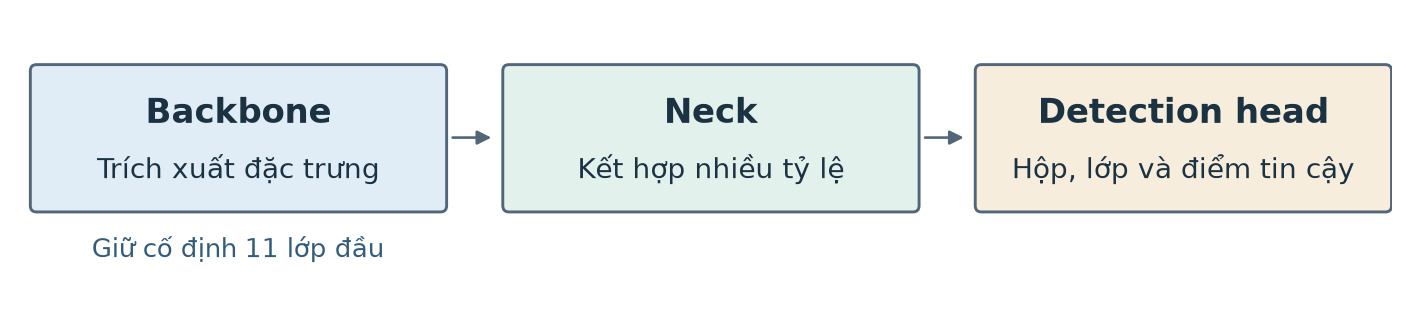
\includegraphics[width=0.92\textwidth]{figures/hinh-2-1-yolo.png}
\caption[Kiến trúc tổng quát của mô hình YOLO]{Kiến trúc tổng quát của mô hình YOLO. Khi tinh chỉnh YOLO26s với dữ liệu biển số, nhóm giữ cố định 11 lớp đầu thuộc backbone và chỉ cập nhật các lớp phía sau}
\label{fig:2-1}
\end{figure}

Với mặt người ở xa, kích thước ảnh đưa vào mạng quyết định còn lại bao nhiêu chi tiết sau khi thu nhỏ. Nhóm thử cùng một bộ trọng số YOLO11n ở hai kích thước, chọn ngưỡng sao cho precision mặt gần bằng nhau (0,781 và 0,780). Khi tăng từ 640 lên 1280 px, recall mặt tăng từ 0,477 lên 0,688, tức 21,1 điểm phần trăm.

\textbf{Ứng dụng trong dự án.} RedactFunnel dùng hai mô hình YOLO26n và YOLO26s tinh chỉnh ở 1280 px, ứng với hai chế độ phát hiện. Quá trình chọn mô hình được trình bày ở mục 4.3.

\subsubsection{Các chỉ số đánh giá mô hình phát hiện}

Gọi $G$ là hộp nhãn do người gán và $B$ là hộp dự đoán. Độ giao trên hợp (\textit{Intersection over Union}, IoU) đo mức trùng khớp của hai hộp:
\[
\operatorname{IoU}(B,G)=\frac{|B\cap G|}{|B\cup G|}.
\]

Với mỗi lớp, các dự đoán được xếp theo điểm tin cậy giảm dần, mỗi hộp nhãn được ghép với nhiều nhất một dự đoán. Cặp ghép có $\operatorname{IoU}\ge 0{,}5$ được tính là đúng ($TP$), dự đoán thừa là $FP$, đối tượng bị bỏ sót là $FN$. Precision cho biết trong các phát hiện được giữ lại có bao nhiêu phần đúng, recall cho biết trong các đối tượng cần tìm đã tìm được bao nhiêu, còn $F_1$ là trung bình điều hoà của hai đại lượng này:
\[
P=\frac{TP}{TP+FP},\qquad R=\frac{TP}{TP+FN},\qquad F_1=\frac{2PR}{P+R}.
\]

Thay đổi ngưỡng điểm tin cậy sẽ tạo ra đường precision--recall. $\mathrm{AP}_{50}$ là diện tích dưới đường này của một lớp khi ngưỡng IoU bằng 0,5, và $\mathrm{mAP}_{50}$ là trung bình $\mathrm{AP}_{50}$ của hai lớp. AP gộp nhiều ngưỡng, trong khi ảnh thật chỉ được xử lý ở một ngưỡng. Vì vậy khi so hai mô hình, nhóm chọn ngưỡng để precision mặt gần bằng nhau rồi so recall. Cách này cho biết mô hình nào tìm được nhiều mặt hơn với cùng mức báo nhầm.

Với bài toán ẩn danh, điều cần biết hơn cả là bao nhiêu diện tích của đối tượng đã được che. Trên một ảnh, gọi $M$ là hợp của các hộp che cùng lớp sau khi nới biên. Độ che phủ của hộp nhãn $G$ là $C(G)=|G\cap M|/|G|$. Với $N$ hộp nhãn, tỷ lệ đối tượng đạt tiêu chí che được định nghĩa là
\[
R_{\mathrm{privacy}}=\frac{1}{N}\sum_{i=1}^{N}\mathbf{1}\!\left[C(G_i)\ge 0{,}70\right].
\]

\begin{figure}[!htbp]
\centering
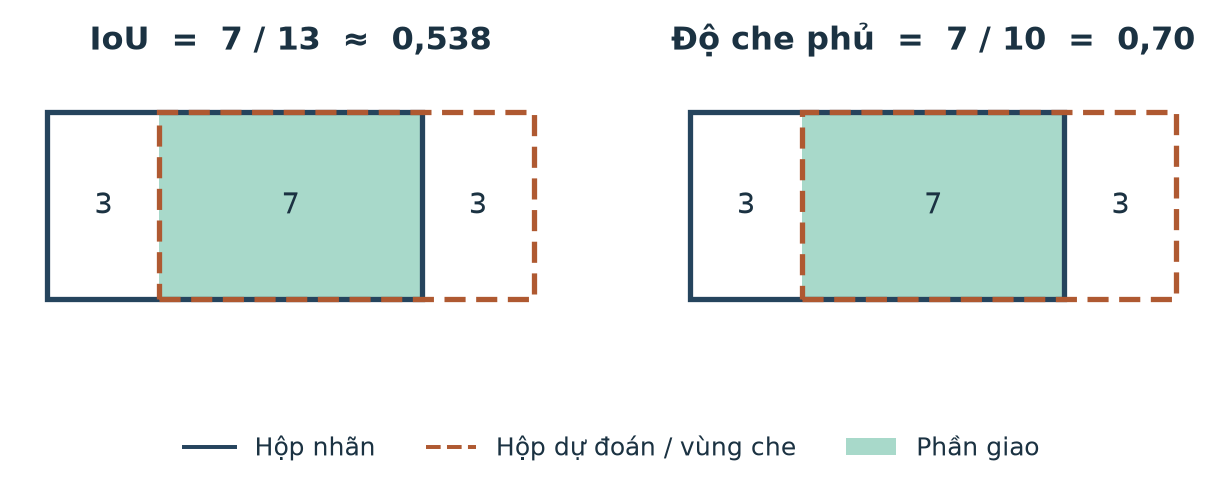
\includegraphics[width=0.85\textwidth]{figures/hinh-2-2-iou-che-phu.png}
\caption[IoU và độ che phủ]{IoU và độ che phủ của cùng một cặp hộp. Hai hộp rộng 10 đơn vị, lệch nhau 3 đơn vị: IoU bằng $7/13$, còn độ che phủ bằng $7/10$, vừa đạt ngưỡng 70\%}
\label{fig:2-2}
\end{figure}

Hai loại lỗi có hậu quả rất khác nhau. Một khuôn mặt bị bỏ sót sẽ xuất hiện nguyên vẹn trong ảnh công bố, còn một vùng nền bị che nhầm chỉ làm mất chi tiết. Vì vậy nhóm ưu tiên giảm bỏ sót, đồng thời theo dõi precision để việc che nhầm không quá nhiều. Ngưỡng 70\% là quy ước của đề tài. Việc có nhận ra người hay đọc được biển hay không còn phụ thuộc phần nào còn nhìn thấy và độ mạnh của phép che.

\textbf{Ứng dụng trong dự án.} Mọi mô hình và công cụ ở Chương 4 đều được so trên cùng tập ảnh, ở cùng mức precision, theo tỷ lệ đối tượng đạt tiêu chí che.

\subsubsection{Nhận diện khuôn mặt bằng vector đặc trưng (face embedding)}

Để biết một khuôn mặt có thuộc danh sách miễn che hay không, mạng nhận diện ánh xạ khuôn mặt thành một vector đặc trưng. ArcFace (Deng và cộng sự, 2019) là phương pháp huấn luyện thêm một biên góc vào hàm mất mát, giúp các danh tính tách xa nhau hơn trong không gian đặc trưng. RedactFunnel dùng mạng MobileFaceNet có sẵn trọng số, chạy bằng ONNX Runtime, sinh vector 512 chiều đã chuẩn hoá $L_2$.

Góc nghiêng của đầu và vị trí mắt thường khác nhau giữa ảnh tham chiếu và ảnh cần che. Trước khi tính vector, YuNet tìm năm điểm mốc gồm hai mắt, đầu mũi và hai khoé miệng. Từ đó hệ thống xoay và co giãn khuôn mặt về vị trí chuẩn trên ảnh $112\times112$ px. Nếu không tìm đủ điểm mốc, vùng mặt được đổi kích thước trực tiếp. Tác động của bước căn chỉnh được đánh giá ở mục 4.7.

Với vector $\mathbf{u}$ của khuôn mặt đang xét và vector tham chiếu $\mathbf{v}$, độ tương đồng cosine là
\[
s(\mathbf{u},\mathbf{v})=\frac{\mathbf{u}^{\mathsf T}\mathbf{v}}{\|\mathbf{u}\|_2\,\|\mathbf{v}\|_2}.
\]

Hệ thống lấy điểm cao nhất trong các ảnh tham chiếu và so với ngưỡng mặc định 0,45. Người lạ vượt ngưỡng sẽ bị giữ rõ nhầm, còn người trong danh sách không đạt ngưỡng sẽ bị che. Ở đây cần phân biệt hai ngưỡng: hạ ngưỡng phát hiện giúp tìm thêm mặt cần bảo vệ, nhưng hạ ngưỡng so khớp lại có thể để lọt người lạ. Vì thế hai ngưỡng được đánh giá riêng.

\textbf{Ứng dụng trong dự án.} ArcFace và YuNet chỉ được dùng khi người dùng tải lên ảnh mẫu. Nếu chỉ yêu cầu che toàn bộ khuôn mặt, hệ thống bỏ qua bước này.

\subsubsection{Nhận dạng ký tự quang học cho biển số Việt Nam}

Biển số dài của ô tô có một dòng, đọc từ trái sang phải. Biển vuông của xe máy và một số ô tô có hai dòng, nên bộ nhận dạng phải giữ đúng thứ tự dòng trên rồi mới đến dòng dưới (Hình~\ref{fig:2-3}). Ngoài bố cục, màu nền cũng khác nhau, ví dụ biển nền vàng của xe kinh doanh vận tải hay biển nền xanh của xe công vụ, khiến độ tương phản của chữ thay đổi.

\begin{figure}[!htbp]
\centering
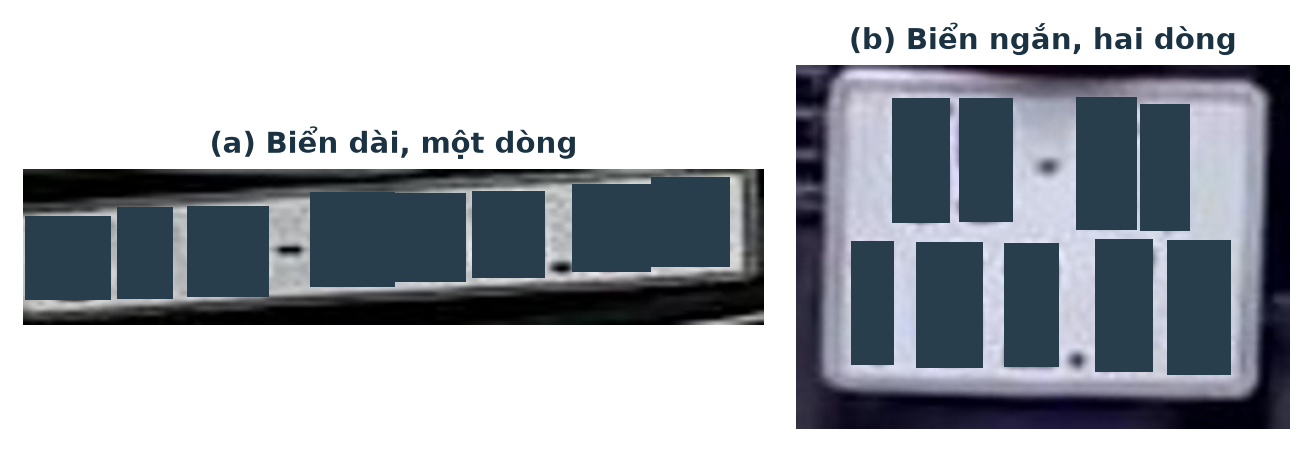
\includegraphics[width=0.8\textwidth]{figures/hinh-2-3-bien-so.png}
\caption[Các dạng biển số Việt Nam]{Hai dạng biển số Việt Nam: (a) biển dài một dòng, (b) biển vuông hai dòng. Ký tự được phủ ô đậm để không lộ số đăng ký}
\label{fig:2-3}
\end{figure}

Do YOLO đã xác định vị trí biển, hệ thống chỉ dùng phần nhận dạng của PP-OCRv4 thông qua RapidOCR, bỏ qua bước phát hiện chữ. Bộ nhận dạng này đọc mỗi lần một dòng, nên mỗi biển được đọc theo hai cách: đọc nguyên vùng biển, và chia đôi theo chiều cao rồi đọc từng nửa. Ảnh đưa vào được kéo ngang 1,3 lần để các chữ số giống nhau đứng cạnh nhau không bị gộp. Cách đọc nào có điểm tin cậy cao hơn thì được chọn.

Sau khi đọc, chuỗi được chuyển thành chữ hoa và bỏ dấu phân cách. Biển chỉ được miễn che khi điểm OCR từ 0,50 trở lên và chuỗi khớp với danh sách. Vì một lần đọc sai vẫn có thể tạo ra chuỗi giống biển được phép, mục 4.6 đánh giá riêng độ chính xác khi đọc và tỷ lệ miễn che nhầm.

\textbf{Ứng dụng trong dự án.} RapidOCR chạy trên ONNX Runtime, dùng chung môi trường với ArcFace nên không phải thêm một thư viện suy luận khác.

\subsubsection{Theo dõi đối tượng và xử lý video}

Trong video hành trình, một biển số có thể rõ ở khung này nhưng nhoè ở khung kế tiếp. Nếu xử lý từng khung riêng lẻ, vết che có thể biến mất đúng lúc điểm phát hiện giảm. ByteTrack (Zhang và cộng sự, 2022) giải quyết việc này bằng cách nối các hộp qua thời gian thành quỹ đạo. Bộ lọc Kalman dự báo vị trí ở khung kế tiếp, các quỹ đạo được ghép với phát hiện điểm cao trước, rồi mới dùng phát hiện điểm thấp để nối những quỹ đạo còn lại. Một mã quỹ đạo cho biết đối tượng liên tục trong đoạn video, nhưng việc đối tượng có được miễn che hay không vẫn phải dựa vào khuôn mặt hoặc biển số.

RedactFunnel xử lý video hai lượt. Lượt đầu phát hiện, nối quỹ đạo và lưu lại các vùng ảnh tốt nhất để xét miễn che. Lượt sau dựng vết che trên từng khung và nội suy ở những khoảng mất dấu ngắn. Phát hiện chưa được ByteTrack gán mã vẫn được che, nên một người chỉ xuất hiện thoáng qua cũng không bị bỏ sót.

Về tệp video, công cụ ffprobe đọc độ phân giải, tốc độ khung hình và luồng âm thanh, OpenCV giải mã từng khung, còn FFmpeg mã hoá kết quả theo chuẩn H.264. Âm thanh gốc được ghép lại nguyên vẹn, không mã hoá lại, và siêu dữ liệu của tệp nguồn được xoá. Thời gian xử lý tăng theo thời lượng video, trong khi một job ảnh chỉ có một ảnh.

\textbf{Ứng dụng trong dự án.} Sự khác biệt này là lý do nhóm tách hàng đợi ảnh và video thành hai nhóm worker, co giãn độc lập với nhau như trình bày ở Chương 3.



\subsection{Backend và xử lý phân tán}


\subsubsection{Kiến trúc hướng sự kiện và NATS JetStream}

{\small\itshape\noindent\textbf{Ghi chú biên soạn:} Nội dung: Message broker, at-least-once delivery, ack / ack\_wait / max\_deliver, retention workqueue; so sánh với Redis Streams, RabbitMQ, Kafka.\par\vspace{6pt}}


\subsubsection{Lưu trữ dữ liệu: PostgreSQL và MinIO}

{\small\itshape\noindent\textbf{Ghi chú biên soạn:} Nội dung: PostgreSQL làm nguồn sự thật cho batch/job; MinIO (object storage tương thích S3), multipart upload, presigned URL.\par\vspace{6pt}}


\subsection{Hạ tầng và Web}


\subsubsection{Kubernetes và KEDA}

{\small\itshape\noindent\textbf{Ghi chú biên soạn:} Nội dung: Chỉ ở mức đủ để hiểu vì sao RedactFunnel dùng: Deployment, PVC, KEDA ScaledObject co giãn theo số job chờ trên NATS (khác HPA co giãn theo CPU/RAM) và scale-to-zero. Không giải thích toàn bộ cách Kubernetes hoạt động.\par\vspace{6pt}}


\subsubsection{Công nghệ phát triển Web}

{\small\itshape\noindent\textbf{Ghi chú biên soạn:} Nội dung: Frontend: React, Vite, TypeScript, React Router. Backend: Node.js, Express, Prisma ORM, Zod, JWT + refresh token, express-rate-limit, multer, archiver; kiểm thử bằng Vitest.\par\vspace{6pt}}


\clearpage
\section{Phân tích và thiết kế hệ thống}
\label{sec:ch3}


\subsection{Tổng quan hệ thống và các tác nhân}

{\small\itshape\noindent\textbf{Ghi chú biên soạn:} Nội dung: Tác nhân: Người dùng (đã đăng ký bằng REGISTER\_KEY), Quản trị viên (cấu hình qua biến môi trường: RETENTION\_DAYS, giới hạn batch), Engine worker (tác nhân hệ thống). Ba khối: Web (frontend + backend), Engine, Infra.\par\vspace{6pt}}


\subsection{Kiến trúc tổng thể}

{\small\itshape\noindent\textbf{Ghi chú biên soạn:} Nội dung: Web không bao giờ chạy model; ghi file lên MinIO, tạo job trong PostgreSQL, publish lệnh lên NATS; worker xử lý và báo sự kiện về jobs.events; KEDA co giãn hai pool ảnh/video độc lập.  Nguồn: docs/architecture.md, Arch.png / Arch.excalidraw, docs/report-material/decisions.md (A)\par\vspace{6pt}}


\begin{figure}[htbp]
\centering
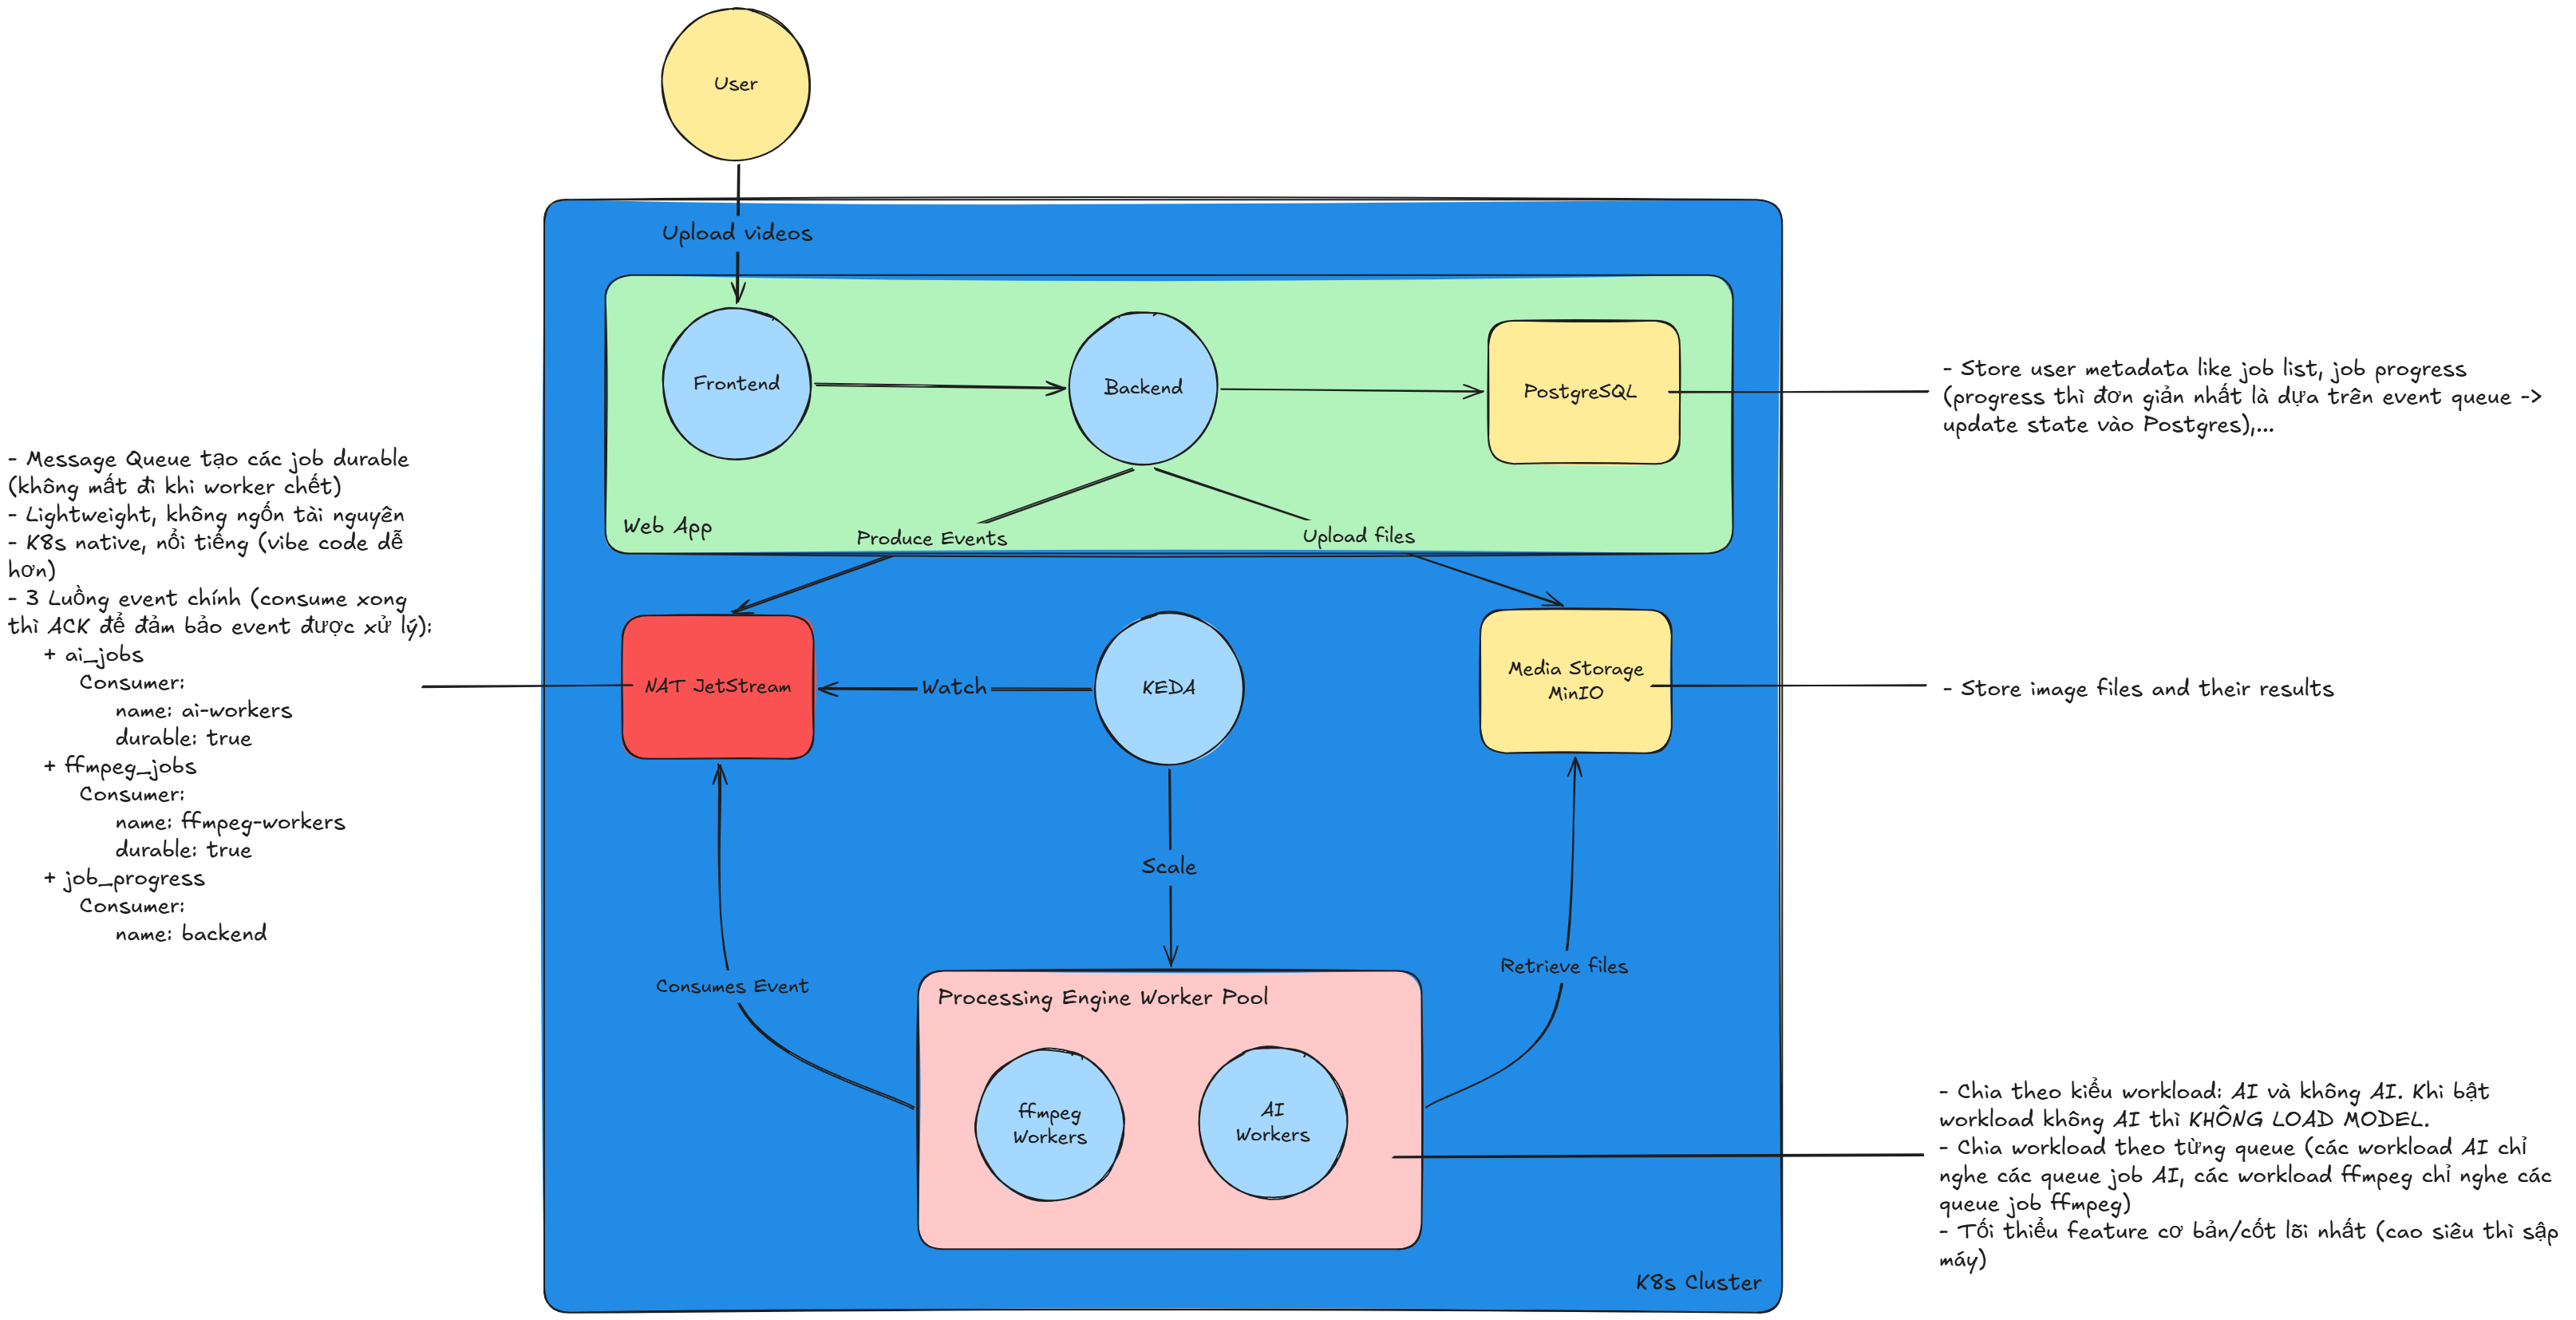
\includegraphics[width=0.88\textwidth]{figures/Arch.png}
\vspace{4pt}
{\small\itshape [HÌNH 3.1]Trình duyệt $\rightarrow$ Gateway/Tunnel $\rightarrow$ Web (React + Express) $\rightarrow$ PostgreSQL, MinIO, NATS (IMAGE\_JOBS, VIDEO\_JOBS, JOB\_EVENTS) $\rightarrow$ image-worker / video-worker (KEDA).Nguồn: Arch.png\par}
\caption{Sơ đồ kiến trúc tổng thể hệ thống RedactFunnel}
\label{fig:3-1}
\end{figure}


\begin{figure}[htbp]
\centering
\fbox{\parbox{0.92\textwidth}{\centering\small\itshape [HÌNH 3.2]Upload $\rightarrow$ tạo job $\rightarrow$ publish jobs.image / jobs.video $\rightarrow$ worker $\rightarrow$ MinIO results $\rightarrow$ jobs.events $\rightarrow$ cập nhật PostgreSQL $\rightarrow$ UI.}}
\caption{Luồng dữ liệu end-to-end của một batch}
\label{fig:3-2}
\end{figure}


\subsection{Đặc tả yêu cầu}


\subsubsection{Yêu cầu chức năng}

\needspace{8\baselineskip}
{\bangfont
\begin{longtable}{|>{\raggedright\arraybackslash\bfseries}m{3.01cm}|>{\raggedright\arraybackslash}m{2.81cm}|>{\raggedright\arraybackslash}m{2.81cm}|>{\raggedright\arraybackslash}m{2.81cm}|>{\raggedright\arraybackslash}m{3.01cm}|}
\caption{Danh sách yêu cầu chức năng}\label{tab:3-1}\\
\hline
\dongdau \textbf{Mã} & \textbf{Nhóm chức năng} & \textbf{Mô tả} & \textbf{Mức ưu tiên} & \textbf{Trạng thái} \\
\hline
\endfirsthead
\multicolumn{5}{c}{\textbf{Bảng 3.1.} Danh sách yêu cầu chức năng (tiếp theo)}\\[2pt]
\hline
\dongdau \textbf{Mã} & \textbf{Nhóm chức năng} & \textbf{Mô tả} & \textbf{Mức ưu tiên} & \textbf{Trạng thái} \\
\hline
\endhead
\endfoot
\endlastfoot
 &  &  &  & \\ \hline
 &  &  &  & \\ \hline
\end{longtable}
}
\vspace{6pt}

{\small\itshape\noindent\textbf{Ghi chú biên soạn:} Nhóm: tài khoản; tạo batch ảnh/video; cấu hình che (đối tượng, kiểu blur/pixelate/blackout, độ mạnh, định dạng/chất lượng xuất, ngưỡng); whitelist khuôn mặt và biển số; theo dõi và thử lại; xem kết quả + báo cáo; sửa ảnh; thư viện media; tải zip; xoá dữ liệu. Trạng thái lấy từ plan.md (Must/Should/Could, [x]).  Nguồn: web/docs/plan.md, engine/docs/plan.md\par\vspace{6pt}}


\subsubsection{Yêu cầu phi chức năng}

\needspace{12\baselineskip}
{\bangfont
\begin{longtable}{|>{\raggedright\arraybackslash\bfseries}m{3.47cm}|>{\raggedright\arraybackslash}m{5.45cm}|>{\raggedright\arraybackslash}m{6.14cm}|}
\caption{Danh sách yêu cầu phi chức năng}\label{tab:3-2}\\
\hline
\dongdau \textbf{Thuộc tính} & \textbf{Yêu cầu} & \textbf{Cách đáp ứng} \\
\hline
\endfirsthead
\multicolumn{3}{c}{\textbf{Bảng 3.2.} Danh sách yêu cầu phi chức năng (tiếp theo)}\\[2pt]
\hline
\dongdau \textbf{Thuộc tính} & \textbf{Yêu cầu} & \textbf{Cách đáp ứng} \\
\hline
\endhead
\endfoot
\endlastfoot
Quyền riêng tư &  & \\ \hline
Độ tin cậy &  & \\ \hline
Khả năng mở rộng &  & \\ \hline
Hiệu năng &  & \\ \hline
Tài nguyên &  & \\ \hline
Bảo trì / triển khai &  & \\ \hline
\end{longtable}
}
\vspace{6pt}

{\small\itshape\noindent\textbf{Ghi chú biên soạn:} Bảo mật \& quyền riêng tư (presigned URL, không public ảnh mẫu, xoá EXIF), tin cậy (không mất job), khả năng mở rộng (scale 0$\rightarrow$N), hiệu năng, ngân sách tài nguyên $\le$ 2,5 GiB RAM nền, khả năng bảo trì.\par\vspace{6pt}}


\subsection{Biểu đồ ca sử dụng}


\begin{figure}[htbp]
\centering
\fbox{\parbox{0.92\textwidth}{\centering\small\itshape [HÌNH 3.3]Use case diagram: Người dùng, Quản trị viên, Engine worker và các nhóm ca sử dụng chính.}}
\caption{Biểu đồ ca sử dụng tổng quát}
\label{fig:3-3}
\end{figure}

\needspace{8\baselineskip}
{\bangfont
\begin{longtable}{|>{\raggedright\arraybackslash\bfseries}m{2.43cm}|>{\raggedright\arraybackslash}m{4.08cm}|>{\raggedright\arraybackslash}m{4.37cm}|>{\raggedright\arraybackslash}m{3.88cm}|}
\caption{Danh sách các ca sử dụng}\label{tab:3-3}\\
\hline
\dongdau \textbf{Mã} & \textbf{Tên ca sử dụng} & \textbf{Tác nhân} & \textbf{Mô tả ngắn} \\
\hline
\endfirsthead
\multicolumn{4}{c}{\textbf{Bảng 3.3.} Danh sách các ca sử dụng (tiếp theo)}\\[2pt]
\hline
\dongdau \textbf{Mã} & \textbf{Tên ca sử dụng} & \textbf{Tác nhân} & \textbf{Mô tả ngắn} \\
\hline
\endhead
\endfoot
\endlastfoot
 &  &  & \\ \hline
 &  &  & \\ \hline
\end{longtable}
}
\vspace{6pt}

{\small\itshape\noindent\textbf{Ghi chú biên soạn:} Liệt kê toàn bộ ca sử dụng, kể cả đăng ký, đăng nhập và thư viện media; chỉ các ca thể hiện thiết kế đặc thù (mục 3.5) được đặc tả chi tiết.\par\vspace{6pt}}


\subsection{Đặc tả các ca sử dụng chính}

{\small\itshape\noindent\textbf{Ghi chú biên soạn:} Nội dung: Mỗi ca sử dụng có bảng đặc tả. Biểu đồ hoạt động và biểu đồ tuần tự chỉ vẽ cho những ca có luồng đặc thù: UC01 có cả hai, UC02 có biểu đồ tuần tự (pipeline video khác ảnh), UC04 có biểu đồ hoạt động.\par\vspace{6pt}}


\subsubsection{UC01. Tạo batch ảnh và tải lên browser}

{\small\itshape\noindent\textbf{Ghi chú biên soạn:} Nội dung: Batch nháp $\rightarrow$ tải từng file một (2 luồng song song, xử lý 429 Retry-After, BATCH\_FULL) $\rightarrow$ start; chọn cả thư mục; cấu hình che có ảnh xem trước.  Nguồn: docs/report-material/decisions.md (F.1)\par\vspace{6pt}}

\needspace{12\baselineskip}
{\bangfont
\begin{longtable}{|>{\raggedright\arraybackslash\bfseries}m{4.04cm}|>{\raggedright\arraybackslash}m{11.31cm}|}
\caption{Đặc tả ca sử dụng Tạo batch ảnh và tải lên}\label{tab:3-4}\\
\hline
\dongdau \textbf{Mục} & \textbf{Nội dung} \\
\hline
\endfirsthead
\multicolumn{2}{c}{\textbf{Bảng 3.4.} Đặc tả ca sử dụng Tạo batch ảnh và tải lên (tiếp theo)}\\[2pt]
\hline
\dongdau \textbf{Mục} & \textbf{Nội dung} \\
\hline
\endhead
\endfoot
\endlastfoot
Mã & UC01 \\ \hline
Tác nhân & \\ \hline
Tiền điều kiện & \\ \hline
Luồng sự kiện chính & \\ \hline
Luồng thay thế / ngoại lệ & \\ \hline
Hậu điều kiện & \\ \hline
\end{longtable}
}
\vspace{6pt}

{\small\itshape\noindent\textbf{Ghi chú biên soạn:} Điền theo mẫu đặc tả: tác nhân, tiền điều kiện, luồng chính, luồng thay thế/ngoại lệ, hậu điều kiện.\par\vspace{6pt}}


\begin{figure}[htbp]
\centering
\fbox{\parbox{0.92\textwidth}{\centering\small\itshape [HÌNH 3.4]Activity diagram (swimlane: Người dùng / Frontend / Backend / NATS / Worker).}}
\caption{Biểu đồ hoạt động ca sử dụng Tạo batch ảnh và tải lên}
\label{fig:3-4}
\end{figure}


\begin{figure}[htbp]
\centering
\fbox{\parbox{0.92\textwidth}{\centering\small\itshape [HÌNH 3.5]Sequence diagram giữa các thành phần tham gia (trình duyệt, Express API, PostgreSQL, MinIO, NATS, Engine worker).}}
\caption{Biểu đồ tuần tự ca sử dụng Tạo batch ảnh và tải lên}
\label{fig:3-5}
\end{figure}

{\small\itshape\noindent\textbf{Ghi chú biên soạn:} Ghi chú khi vẽ: Mỗi mũi tên ghi tên hàm thật trong code kèm schema hoặc kiểu dữ liệu của tham số, dạng hàm(schema). Ví dụ luồng này: createDraftBatch(whitelist: File[], config), backend kiểm tra config bằng batchConfigSchema $\rightarrow$ createBatchHandler $\rightarrow$ createDraftBatch(...) lưu Batch; uploadFileToBatch(batchId, File) $\rightarrow$ addBatchFileHandler $\rightarrow$ addBatchFile(...) tạo Job; startBatch(batchId) $\rightarrow$ startBatchHandler $\rightarrow$ startBatch(batchId, userId) $\rightarrow$ publishJob("jobs.image", ImageRedactCommand); Engine: EngineWorker.handle\_job(msg) $\rightarrow$ ImageRedactProcessor.process(input\_bytes, params) $\rightarrow$ StorageClient.upload\_file(...) $\rightarrow$ MessagingClient.emit\_completion\_event(job\_id, output\_bucket, output\_key, result\_summary); Backend: applyJobEvent(ValidatedJobEvent).  Nguồn: web/frontend/src/api.ts, web/backend/src/services/batch.service.ts, web/backend/src/messaging.ts, web/backend/src/domain/command.ts, engine/src/main.py, engine/src/processors/image\_redact.py\par\vspace{6pt}}


\subsubsection{UC02. Tải lên và bắt đầu batch xử lý video}

{\small\itshape\noindent\textbf{Ghi chú biên soạn:} Nội dung: Upload multipart 8 MB/phần, kiểm tra kích thước + ffprobe (H.264, 15-60 s) trước khi tạo job video-redact, theo dõi tiến độ theo khung hình.  Nguồn: decisions.md (F.1), engine/src/processors/video\_redact.py\par\vspace{6pt}}

\needspace{12\baselineskip}
{\bangfont
\begin{longtable}{|>{\raggedright\arraybackslash\bfseries}m{4.04cm}|>{\raggedright\arraybackslash}m{11.31cm}|}
\caption{Đặc tả ca sử dụng Tải lên và bắt đầu batch xử lý video}\label{tab:3-5}\\
\hline
\dongdau \textbf{Mục} & \textbf{Nội dung} \\
\hline
\endfirsthead
\multicolumn{2}{c}{\textbf{Bảng 3.5.} Đặc tả ca sử dụng Tải lên và bắt đầu batch xử lý video (tiếp theo)}\\[2pt]
\hline
\dongdau \textbf{Mục} & \textbf{Nội dung} \\
\hline
\endhead
\endfoot
\endlastfoot
Mã & UC02 \\ \hline
Tác nhân & \\ \hline
Tiền điều kiện & \\ \hline
Luồng sự kiện chính & \\ \hline
Luồng thay thế / ngoại lệ & \\ \hline
Hậu điều kiện & \\ \hline
\end{longtable}
}
\vspace{6pt}

{\small\itshape\noindent\textbf{Ghi chú biên soạn:} Điền theo mẫu đặc tả: tác nhân, tiền điều kiện, luồng chính, luồng thay thế/ngoại lệ, hậu điều kiện.\par\vspace{6pt}}


\begin{figure}[htbp]
\centering
\fbox{\parbox{0.92\textwidth}{\centering\small\itshape [HÌNH 3.6]Sequence diagram giữa các thành phần tham gia (trình duyệt, Express API, PostgreSQL, MinIO, NATS, Engine worker).}}
\caption{Biểu đồ tuần tự ca sử dụng Tải lên và xử lý video}
\label{fig:3-6}
\end{figure}

{\small\itshape\noindent\textbf{Ghi chú biên soạn:} Ghi chú khi vẽ: Mỗi mũi tên ghi tên hàm thật trong code kèm schema hoặc kiểu dữ liệu của tham số, dạng hàm(schema). Ví dụ luồng này: uploadVideoToBatch(batchId, File) $\rightarrow$ startUploadHandler $\rightarrow$ beginMultipartUpload(...) tạo UploadSession; mỗi phần 8 MB: uploadPartHandler $\rightarrow$ writeMultipartPart(...); completeUploadHandler $\rightarrow$ finishMultipartUpload(...) $\rightarrow$ validateUploadedVideo(objectKey); startBatch(batchId, userId) $\rightarrow$ publishJob("jobs.video", VideoRedactCommand); Engine: EngineWorker.handle\_job(msg) $\rightarrow$ VideoRedactProcessor.process(input\_bytes, params, progress\_callback) $\rightarrow$ MessagingClient.emit\_progress\_event(job\_id, progress) $\rightarrow$ emit\_completion\_event(...); Backend: applyJobEvent(ValidatedJobEvent).  Nguồn: web/frontend/src/api.ts, web/backend/src/services/upload.service.ts, web/backend/src/services/video-validation.service.ts, web/backend/src/domain/command.ts, engine/src/main.py, engine/src/processors/video\_redact.py\par\vspace{6pt}}


\subsubsection{UC03. Theo dõi batch và thử lại ảnh lỗi}

{\small\itshape\noindent\textbf{Ghi chú biên soạn:} Nội dung: Đồng bộ trạng thái từ jobs.events (idempotent), tiến độ tổng, thử lại ảnh FAILED, xử lý 409 WHITELIST\_FACES\_MISSING.  Nguồn: docs/integration-contracts.md §8\par\vspace{6pt}}

\needspace{12\baselineskip}
{\bangfont
\begin{longtable}{|>{\raggedright\arraybackslash\bfseries}m{4.04cm}|>{\raggedright\arraybackslash}m{11.31cm}|}
\caption{Đặc tả ca sử dụng Theo dõi batch và thử lại ảnh lỗi}\label{tab:3-6}\\
\hline
\dongdau \textbf{Mục} & \textbf{Nội dung} \\
\hline
\endfirsthead
\multicolumn{2}{c}{\textbf{Bảng 3.6.} Đặc tả ca sử dụng Theo dõi batch và thử lại ảnh lỗi (tiếp theo)}\\[2pt]
\hline
\dongdau \textbf{Mục} & \textbf{Nội dung} \\
\hline
\endhead
\endfoot
\endlastfoot
Mã & UC03 \\ \hline
Tác nhân & \\ \hline
Tiền điều kiện & \\ \hline
Luồng sự kiện chính & \\ \hline
Luồng thay thế / ngoại lệ & \\ \hline
Hậu điều kiện & \\ \hline
\end{longtable}
}
\vspace{6pt}

{\small\itshape\noindent\textbf{Ghi chú biên soạn:} Điền theo mẫu đặc tả: tác nhân, tiền điều kiện, luồng chính, luồng thay thế/ngoại lệ, hậu điều kiện.\par\vspace{6pt}}


\subsubsection{UC04. Xem kết quả và báo cáo cần xem lại}

{\small\itshape\noindent\textbf{Ghi chú biên soạn:} Nội dung: Thanh trượt before/after, danh sách phát hiện, báo cáo needsReview (confidence thấp, sát ngưỡng whitelist, khoảng mất theo dõi của video), xuất JSON.  Nguồn: decisions.md (D)\par\vspace{6pt}}

\needspace{12\baselineskip}
{\bangfont
\begin{longtable}{|>{\raggedright\arraybackslash\bfseries}m{4.04cm}|>{\raggedright\arraybackslash}m{11.31cm}|}
\caption{Đặc tả ca sử dụng Xem kết quả và báo cáo cần xem lại}\label{tab:3-7}\\
\hline
\dongdau \textbf{Mục} & \textbf{Nội dung} \\
\hline
\endfirsthead
\multicolumn{2}{c}{\textbf{Bảng 3.7.} Đặc tả ca sử dụng Xem kết quả và báo cáo cần xem lại (tiếp theo)}\\[2pt]
\hline
\dongdau \textbf{Mục} & \textbf{Nội dung} \\
\hline
\endhead
\endfoot
\endlastfoot
Mã & UC04 \\ \hline
Tác nhân & \\ \hline
Tiền điều kiện & \\ \hline
Luồng sự kiện chính & \\ \hline
Luồng thay thế / ngoại lệ & \\ \hline
Hậu điều kiện & \\ \hline
\end{longtable}
}
\vspace{6pt}

{\small\itshape\noindent\textbf{Ghi chú biên soạn:} Điền theo mẫu đặc tả: tác nhân, tiền điều kiện, luồng chính, luồng thay thế/ngoại lệ, hậu điều kiện.\par\vspace{6pt}}


\begin{figure}[htbp]
\centering
\fbox{\parbox{0.92\textwidth}{\centering\small\itshape [HÌNH 3.7]Activity diagram (swimlane: Người dùng / Frontend / Backend).}}
\caption{Biểu đồ hoạt động ca sử dụng Xem kết quả và báo cáo cần xem lại}
\label{fig:3-7}
\end{figure}


\subsubsection{UC05. Sửa ảnh và render lại}

{\small\itshape\noindent\textbf{Ghi chú biên soạn:} Nội dung: Bật/tắt box, vẽ thêm box, đổi kiểu che; tạo job image-render từ ảnh gốc, không chạy lại AI.  Nguồn: engine/src/processors/image\_render.py\par\vspace{6pt}}

\needspace{12\baselineskip}
{\bangfont
\begin{longtable}{|>{\raggedright\arraybackslash\bfseries}m{4.04cm}|>{\raggedright\arraybackslash}m{11.31cm}|}
\caption{Đặc tả ca sử dụng Sửa ảnh và render lại}\label{tab:3-8}\\
\hline
\dongdau \textbf{Mục} & \textbf{Nội dung} \\
\hline
\endfirsthead
\multicolumn{2}{c}{\textbf{Bảng 3.8.} Đặc tả ca sử dụng Sửa ảnh và render lại (tiếp theo)}\\[2pt]
\hline
\dongdau \textbf{Mục} & \textbf{Nội dung} \\
\hline
\endhead
\endfoot
\endlastfoot
Mã & UC05 \\ \hline
Tác nhân & \\ \hline
Tiền điều kiện & \\ \hline
Luồng sự kiện chính & \\ \hline
Luồng thay thế / ngoại lệ & \\ \hline
Hậu điều kiện & \\ \hline
\end{longtable}
}
\vspace{6pt}

{\small\itshape\noindent\textbf{Ghi chú biên soạn:} Điền theo mẫu đặc tả: tác nhân, tiền điều kiện, luồng chính, luồng thay thế/ngoại lệ, hậu điều kiện.\par\vspace{6pt}}


\subsubsection{UC06. Quản lý danh sách khuôn mặt và whitelist biển số}

{\small\itshape\noindent\textbf{Ghi chú biên soạn:} Nội dung: Lưu danh sách khuôn mặt opt-in theo tài khoản (allowList), dùng lại khi tạo/chạy lại batch; nhập danh sách biển số được giữ nguyên.  Nguồn: decisions.md (E), web/docs/plan.md\par\vspace{6pt}}

\needspace{12\baselineskip}
{\bangfont
\begin{longtable}{|>{\raggedright\arraybackslash\bfseries}m{4.04cm}|>{\raggedright\arraybackslash}m{11.31cm}|}
\caption{Đặc tả ca sử dụng Quản lý danh sách khuôn mặt và whitelist biển số}\label{tab:3-9}\\
\hline
\dongdau \textbf{Mục} & \textbf{Nội dung} \\
\hline
\endfirsthead
\multicolumn{2}{c}{\textbf{Bảng 3.9.} Đặc tả ca sử dụng Quản lý danh sách khuôn mặt và whitelist biển số (tiếp theo)}\\[2pt]
\hline
\dongdau \textbf{Mục} & \textbf{Nội dung} \\
\hline
\endhead
\endfoot
\endlastfoot
Mã & UC06 \\ \hline
Tác nhân & \\ \hline
Tiền điều kiện & \\ \hline
Luồng sự kiện chính & \\ \hline
Luồng thay thế / ngoại lệ & \\ \hline
Hậu điều kiện & \\ \hline
\end{longtable}
}
\vspace{6pt}

{\small\itshape\noindent\textbf{Ghi chú biên soạn:} Điền theo mẫu đặc tả: tác nhân, tiền điều kiện, luồng chính, luồng thay thế/ngoại lệ, hậu điều kiện.\par\vspace{6pt}}


\subsection{Thiết kế cơ sở dữ liệu}

{\small\itshape\noindent\textbf{Ghi chú biên soạn:} Nội dung: Sáu bảng của Prisma schema: User, Batch, Job, FaceList, RefreshToken, UploadSession và enum JobStatus. Giải thích quan hệ (User 1-n Batch, Batch 1-n Job, User 1-n FaceList\dots{}), các cột JSON (config, resultSummary) và chỉ mục.  Nguồn: web/backend/prisma/schema.prisma\par\vspace{6pt}}


\begin{figure}[htbp]
\centering
\fbox{\parbox{0.92\textwidth}{\centering\small\itshape [HÌNH 3.8]ERD sinh từ schema.prisma (có thể dùng prisma-erd-generator hoặc dbdiagram.io).}}
\caption{Biểu đồ thực thể liên kết (ERD) của cơ sở dữ liệu}
\label{fig:3-8}
\end{figure}


\begin{figure}[htbp]
\centering
\fbox{\parbox{0.92\textwidth}{\centering\small\itshape [HÌNH 3.9]State machine từ PENDING/QUEUED $\rightarrow$ PROCESSING $\rightarrow$ COMPLETED / FAILED, kèm sự kiện gây chuyển trạng thái và thử lại.Nguồn: enum JobStatus trong schema.prisma, docs/integration-contracts.md}}
\caption{Biểu đồ trạng thái của Job (JobStatus)}
\label{fig:3-9}
\end{figure}


\subsection{Thiết kế hợp đồng tích hợp giữa các thành phần}

{\small\itshape\noindent\textbf{Ghi chú biên soạn:} Nội dung: Chỉ nêu các quyết định quan trọng của hợp đồng chung giữa ba nhóm: mỗi ảnh hoặc video là một job riêng; ba stream tách theo loại job để KEDA co giãn hai pool độc lập; ack\_wait và max\_deliver đặt theo thời gian xử lý thật của từng loại job; sự kiện trạng thái được xử lý idempotent; file lưu theo batchId và không bao giờ public. Định dạng chi tiết của từng thông điệp không đưa vào báo cáo.  Nguồn: docs/integration-contracts.md, decisions.md (G.3, G.4)\par\vspace{6pt}}

\needspace{9\baselineskip}
{\bangfont
\begin{longtable}{|>{\raggedright\arraybackslash\bfseries}m{2.55cm}|>{\raggedright\arraybackslash}m{2.15cm}|>{\raggedright\arraybackslash}m{3.45cm}|>{\raggedright\arraybackslash}m{1.95cm}|>{\raggedright\arraybackslash}m{2.35cm}|>{\raggedright\arraybackslash}m{1.65cm}|}
\caption{Các stream, subject và consumer trên NATS JetStream}\label{tab:3-10}\\
\hline
\dongdau \textbf{Stream} & \textbf{Subject} & \textbf{Consumer} & \textbf{Retention} & \textbf{ack\_wait / max\_deliver} & \textbf{Bên đọc} \\
\hline
\endfirsthead
\multicolumn{6}{c}{\textbf{Bảng 3.10.} Các stream, subject và consumer trên NATS JetStream (tiếp theo)}\\[2pt]
\hline
\dongdau \textbf{Stream} & \textbf{Subject} & \textbf{Consumer} & \textbf{Retention} & \textbf{ack\_wait / max\_deliver} & \textbf{Bên đọc} \\
\hline
\endhead
\endfoot
\endlastfoot
IMAGE\_JOBS & jobs.image & image-workers &  &  & \\ \hline
VIDEO\_JOBS & jobs.video & video-workers &  &  & \\ \hline
JOB\_EVENTS & jobs.events & backend-job-events &  &  & \\ \hline
\end{longtable}
}
\vspace{6pt}

{\small\itshape\noindent\textbf{Ghi chú biên soạn:} Ba stream IMAGE\_JOBS, VIDEO\_JOBS, JOB\_EVENTS.  Nguồn: docs/integration-contracts.md §4, decisions.md (G.3, G.4)\par\vspace{6pt}}


\subsection{Thiết kế Engine xử lý}

Engine nhận yêu cầu từ Backend, đọc tệp nguồn trên MinIO và tạo một tệp kết quả đã che. Thiết kế tách thành hai quyết định. Ở cấp job, worker chọn bộ xử lý theo loại công việc. Ở cấp đối tượng, bộ xử lý tìm vùng phải che và chỉ giữ rõ khi đủ điều kiện miễn che. Với ảnh, quyết định gắn với từng hộp phát hiện. Với video, quyết định gắn với cả một đoạn quỹ đạo để vết che không bị ngắt quãng khi đối tượng di chuyển.

\textbf{Hai nhóm worker.} Backend gửi lệnh qua NATS JetStream, trong đó có mã job, loại công việc, tham số và vị trí của tệp vào, tệp ra trên MinIO. Nội dung tệp không đi qua hàng đợi. Khi khởi động, mỗi nhóm worker chỉ đăng ký những bộ xử lý thuộc nhóm của mình:

\begin{center}
\bangfont
\begin{tabular}{|L{2.2cm}|L{2.8cm}|L{10.0cm}|}
\hline
\dongdau \textbf{Nhóm worker} & \textbf{Loại job} & \textbf{Công việc và kết quả trả về} \\ \hline
Ảnh & image-redact & Tìm và che đối tượng. Kết quả ghi từng hộp, quyết định che hay giữ, số mặt, số biển và số phát hiện có điểm thấp. \\ \hline
Ảnh & image-render & Dựng lại ảnh từ các hộp người dùng đã sửa, không chạy mô hình. \\ \hline
Video & video-redact & Che theo thời gian. Kết quả ghi thông tin video, danh sách quỹ đạo và số đếm theo quỹ đạo. Một người có thể tạo nhiều đoạn quỹ đạo. \\ \hline
\end{tabular}
\end{center}

Nhờ tách hai hàng đợi, nhóm ảnh vẫn nhận việc khi nhóm video đang xử lý một clip dài. Điều này quan trọng với chức năng sửa ảnh, vì người dùng đang chờ xem kết quả ngay. KEDA theo dõi số job chờ của từng hàng đợi và co giãn từ 0 đến 3 worker ảnh, từ 0 đến 1 worker video.

\textbf{Vòng đời mô hình và job.} Cả hai bộ xử lý đều chọn trọng số theo chế độ: Fast dùng YOLO26n, Maximum privacy dùng YOLO26s, cùng ở 1280 px. Bộ xử lý ảnh nạp YOLO khi khởi động, bộ xử lý video nạp khi cần suy luận lần đầu. Các job liên tiếp cùng chế độ dùng lại mô hình trong RAM. Nếu job sau cần mô hình khác, mô hình cũ được giải phóng rồi mới nạp mô hình mới. ArcFace và RapidOCR chỉ khởi tạo khi job có danh sách miễn che tương ứng.

Phần suy luận chạy trên luồng riêng để worker vẫn báo được cho JetStream mỗi 15 giây rằng job còn đang chạy. Tiến độ gửi cho Backend đi theo kênh sự kiện riêng. Mỗi job có hạn thời gian: 5 phút với ảnh và 3 giờ với video. Quá hạn, worker báo lỗi \code{JOB\_TIMEOUT} rồi thoát để Kubernetes khởi động lại. Khi thành công, thứ tự luôn là: ghi kết quả lên MinIO, gửi sự kiện hoàn tất, rồi mới xác nhận thông điệp với JetStream. Nhờ thứ tự này, nếu worker chết giữa chừng thì job được giao lại chứ không bị mất.

\textbf{Luồng xử lý ảnh.} Sau khi giải mã ảnh, YOLO chạy ở ngưỡng thấp nhất trong các lớp được yêu cầu, sau đó từng hộp được lọc theo ngưỡng riêng của lớp. Làm hai bước như vậy giữ được những biển số có điểm thấp hơn ngưỡng của khuôn mặt. Hộp đã qua ngưỡng nhưng điểm vẫn thấp sẽ được che và gắn cờ để người dùng xem lại. Hình~\ref{fig:3-10} mô tả toàn bộ luồng.

\begin{figure}[!htbp]
\centering
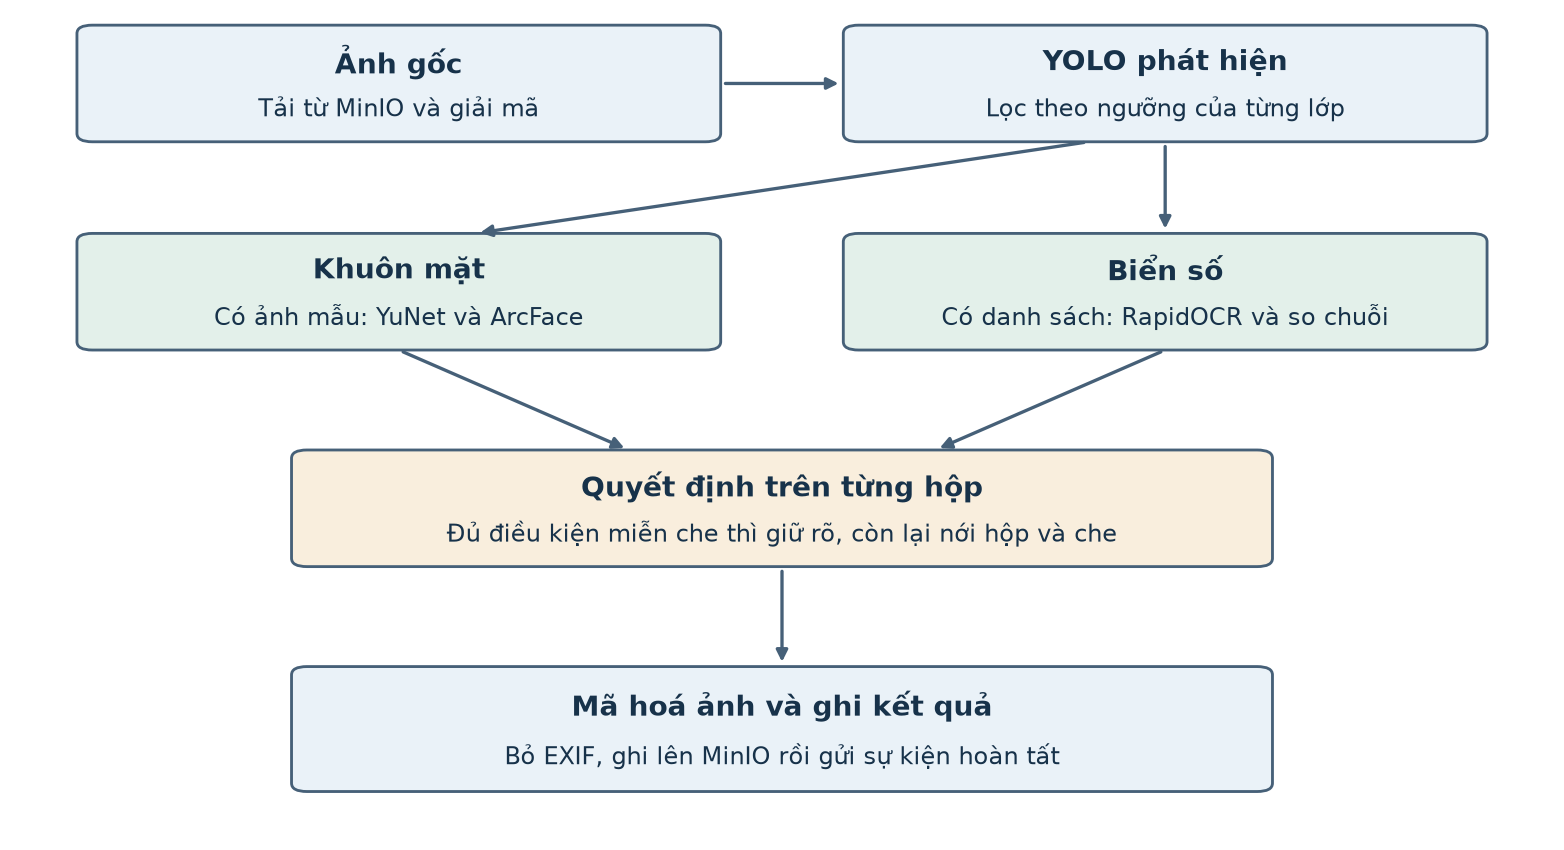
\includegraphics[width=0.95\textwidth]{figures/hinh-3-10-luong-xu-ly-anh.png}
\caption[Luồng xử lý ảnh]{Luồng xử lý ảnh (image-redact). Hai nhánh sau YOLO ứng với khuôn mặt và biển số, chỉ chạy khi có danh sách miễn che}
\label{fig:3-10}
\end{figure}

Ở nhánh khuôn mặt, YuNet căn chỉnh rồi ArcFace so với ảnh mẫu. Ở nhánh biển số, RapidOCR đọc chuỗi rồi so với danh sách. Nguyên tắc chung là mặc định che: điểm tương đồng dưới ngưỡng, OCR không đọc được hay đọc không chắc chắn đều dẫn đến che. Riêng lỗi ở ảnh mẫu, ví dụ ảnh hỏng hoặc không có khuôn mặt, được báo thành lỗi riêng để người dùng biết và thay ảnh.

Với mỗi hộp cần che, vùng che được nới thêm mặc định 10\% mỗi phía. Người dùng chọn làm mờ Gaussian, khảm ô (pixelate) hoặc phủ đen. Độ mạnh được tính theo chiều rộng vùng che, nên khuôn mặt lớn hay nhỏ đều được che như nhau. Ảnh kết quả được mã hoá lại từ điểm ảnh, do đó EXIF và toạ độ GPS của ảnh gốc không còn. Khi người dùng sửa vùng che trên web, hệ thống áp dụng danh sách hộp mới lên ảnh gốc mà không phải chạy lại YOLO.

\textbf{Luồng xử lý video.} Nếu một biển số chỉ đọc rõ ở giữa clip thì quyết định miễn che ngay từ khung đầu sẽ thiếu căn cứ. Vì vậy video được đọc hai lượt: lượt đầu gom bằng chứng trên cả quỹ đạo, lượt sau mới dựng video đầu ra (Hình~\ref{fig:3-11}). Cái giá phải trả là đọc lại video một lần.

\begin{figure}[!htbp]
\centering
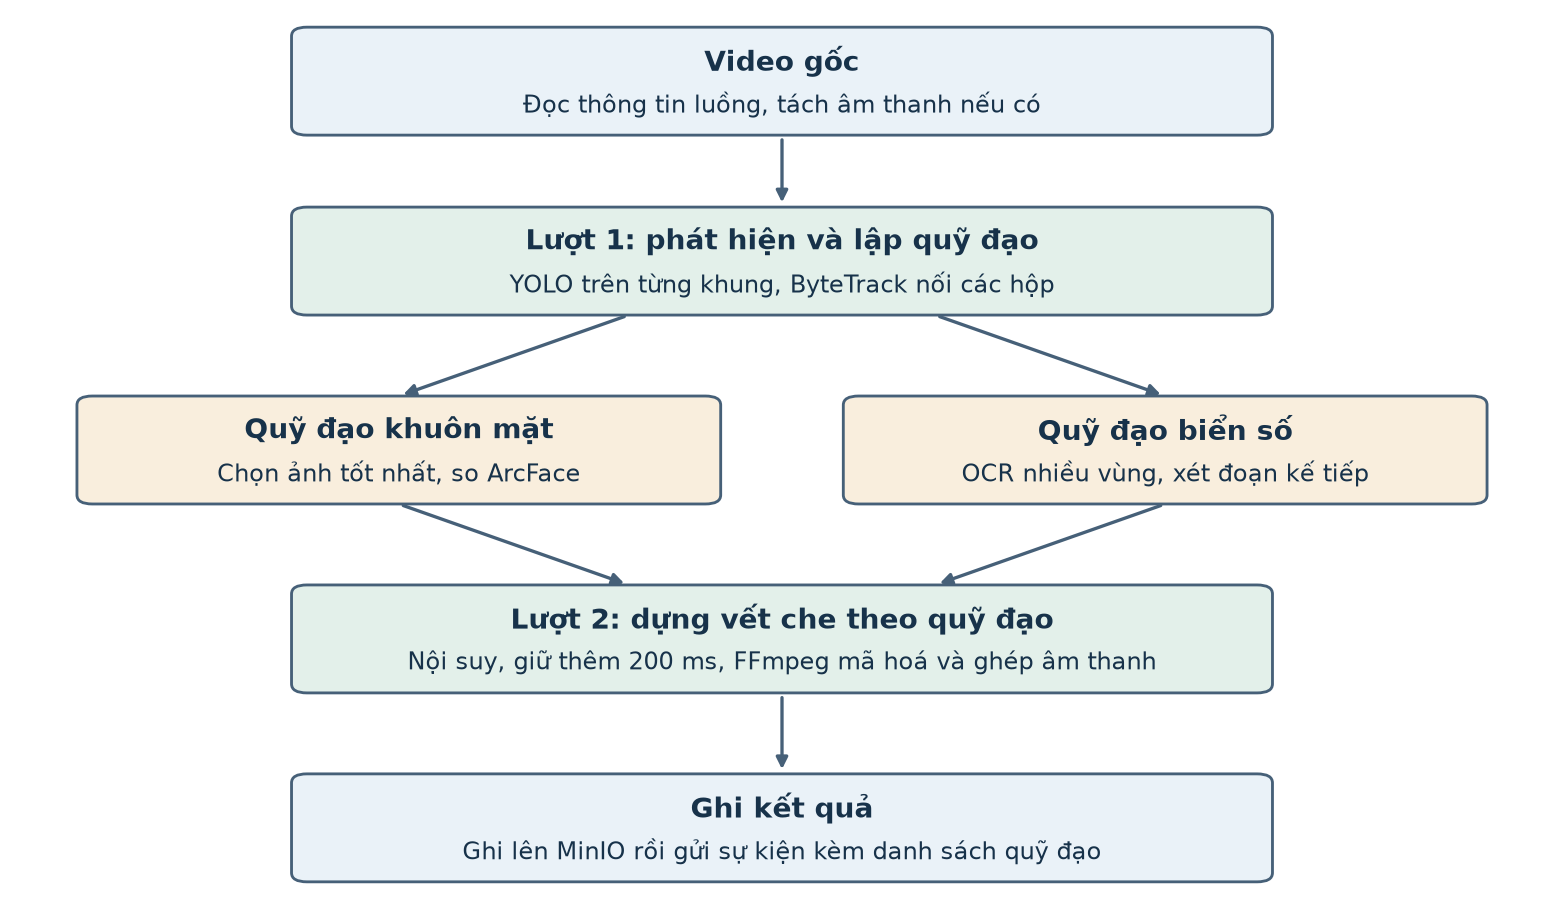
\includegraphics[width=0.95\textwidth]{figures/hinh-3-11-luong-xu-ly-video.png}
\caption[Luồng xử lý video]{Luồng xử lý video (video-redact). Quyết định miễn che nằm giữa lượt theo dõi và lượt dựng video}
\label{fig:3-11}
\end{figure}

Ở lượt đầu, YOLO phát hiện trên từng khung và ByteTrack nối các hộp thành quỹ đạo. Hộp đạt ngưỡng nhưng chưa được cấp mã vẫn được giữ: hệ thống thử ghép với hộp cùng lớp ở khung trước, nếu không được thì cấp mã riêng. Khoảng mất dấu dưới 167 ms được nội suy, còn dài hơn thì tách thành đoạn mới để không nối qua quãng thiếu quan sát. Vết che còn được giữ thêm 200 ms trước và sau mỗi chuỗi phát hiện để không bị nhấp nháy. Hai khoảng thời gian này được đổi ra số khung theo tốc độ của video.

Với khuôn mặt, hệ thống chọn một ảnh tốt nhất của quỹ đạo theo điểm phát hiện, kích thước và độ nét để so với ảnh mẫu. Với biển số, hệ thống đọc ảnh đại diện và tối đa năm vùng cắt rộng nhất, dừng ngay khi khớp. Nếu một biển bị tách thành nhiều đoạn, đoạn nằm gần đoạn đã khớp có thể được kế thừa quyết định, với điều kiện hai đoạn gần nhau về thời gian, vị trí và đoạn đang xét không đọc ra biển khác. Chỉ đoạn khớp OCR trực tiếp mới được làm nguồn kế thừa, nên việc miễn che không lan truyền dây chuyền.

Ở lượt sau, từng khung được đọc lại, áp dụng vết che rồi chuyển cho FFmpeg mã hoá H.264. Âm thanh gốc được ghép lại nguyên vẹn và siêu dữ liệu bị xoá. Cùng với tệp MP4, Backend nhận được thời điểm khung đại diện, các khoảng điểm thấp và các khoảng mất dấu của từng quỹ đạo. Nhờ đó, người dùng có thể nhảy thẳng đến đoạn cần kiểm tra.



\subsection{Thiết kế hạ tầng triển khai}

{\small\itshape\noindent\textbf{Ghi chú biên soạn:} Nội dung: Namespace imgproc trên cụm Lab-sock (k3s), hai pool worker, ScaledObject KEDA, Gateway API cho imgproc.sock1000kg.io.vn và blob-imgproc.sock1000kg.io.vn.  Nguồn: infra/AGENTS.md, infra/app/, infra/cluster/keda, decisions.md (G)\par\vspace{6pt}}


\begin{figure}[htbp]
\centering
\fbox{\parbox{0.92\textwidth}{\centering\small\itshape [HÌNH 3.12]Deployment diagram: namespace imgproc (web, image-worker, video-worker, NATS, PostgreSQL, MinIO, Job setup), namespace keda, Gateway Traefik, cloudflared.}}
\caption{Sơ đồ triển khai trên Kubernetes}
\label{fig:3-12}
\end{figure}


\clearpage
\section{Giải pháp AI: dữ liệu, huấn luyện và đánh giá}
\label{sec:ch4}

Engine phải trả lời ba câu hỏi với mỗi ảnh hoặc video: đối tượng cần che nằm ở đâu, đối tượng nào thuộc danh sách miễn che, và quyết định đó có giữ được qua các khung hình hay không. Chương này trình bày dữ liệu, cách đánh giá và kết quả cho từng câu hỏi, lần lượt từ phát hiện, đọc biển số, xác minh khuôn mặt đến video.

\subsection{Dữ liệu huấn luyện và đánh giá}

Trong bốn bài toán, nhóm chỉ tự huấn luyện bộ phát hiện khuôn mặt và biển số. Bộ trích đặc trưng khuôn mặt, YuNet và PP-OCRv4 dùng trọng số có sẵn, nên dữ liệu của hai bài toán này chỉ để chọn cách dùng và đánh giá. Bảng~\ref{tab:4-1} liệt kê các tập dữ liệu.

{\bangfont
\begin{longtable}{|L{2.0cm}|L{3.8cm}|L{3.6cm}|L{5.2cm}|}
\caption{Thống kê các tập dữ liệu sử dụng}\label{tab:4-1}\\
\hline
\dongdau \textbf{Bài toán} & \textbf{Tập dữ liệu} & \textbf{Quy mô} & \textbf{Vai trò} \\ \hline
\endfirsthead
\multicolumn{4}{c}{\textbf{Bảng 4.1.} (tiếp theo)}\\[2pt]
\hline
\dongdau \textbf{Bài toán} & \textbf{Tập dữ liệu} & \textbf{Quy mô} & \textbf{Vai trò} \\ \hline
\endhead
\endfoot
\endlastfoot
Phát hiện & WIDER FACE train & 12.225 ảnh & Huấn luyện lớp mặt \\ \cline{2-4}
 & Ô cắt từ ảnh đám đông & 236 ô từ 45 ảnh & Huấn luyện, từ bước 3 \\ \cline{2-4}
 & Biển số Việt Nam & 3.428 ảnh & Huấn luyện lớp biển \\ \cline{2-4}
 & Khung camera hành trình & 468 khung, 590 biển & Huấn luyện, bước 8 \\ \cline{2-4}
 & Ảnh đồng hồ xe, không nhãn & 384 ảnh & Mẫu âm của một biến thể bước 8 (bị loại) \\ \cline{2-4}
 & Validation & 610 ảnh mặt, 1.141 ảnh biển & Theo dõi trong lúc huấn luyện \\ \cline{2-4}
 & Bộ đánh giá & 3.226 ảnh WIDER val (39.112 mặt), 500 ảnh biển UET & So sánh mô hình, chọn ngưỡng \\ \hline
Đọc biển số & Tập UET & 80 biển (16 biển hai dòng) & Chọn và kiểm tra cách đọc \\ \cline{2-4}
 & Tập trungdinh & 536 biển (440 biển hai dòng) & So sánh các cách đọc \\ \hline
Xác minh mặt & LFW & 600 chủ thể, 600 người lạ, 3.000 ảnh & Chọn cách căn chỉnh và ngưỡng \\ \hline
Video & 2 clip dashcam, 3 clip điện thoại & 5.952 khung & Tìm lỗi của Engine, đánh giá toàn luồng \\ \hline
\end{longtable}
}

\textbf{Dữ liệu phát hiện.} WIDER FACE (Yang và cộng sự, 2016) có rất nhiều mặt nhỏ và mặt bị che khuất, nhóm tách 5\% phần train làm validation. Có 45 ảnh đám đông trên 300 mặt làm tràn bộ nhớ GPU ở 1280 px, nên nhóm bỏ ở các bước đầu rồi đưa lại dưới dạng 236 ô cắt. Với biển số, chín ảnh gần trùng với bộ đánh giá đã được loại. Bộ đánh giá 3.726 ảnh không tham gia cập nhật trọng số, nhưng nhóm dùng chính nó để so mô hình và chọn ngưỡng. Vì vậy các con số có thể hơi lạc quan so với một tập hoàn toàn mới, và đây là hạn chế của đề tài.

Khung dashcam được thêm vào vì kích thước biển trong dữ liệu cũ khác xa thực tế. Biển trong tập huấn luyện là ảnh cận cảnh, rộng trung bình khoảng 21\% chiều rộng ảnh (trong bộ đánh giá là 18\%), còn trên dashcam chỉ 3,2\%, và 76\% số biển nhỏ hơn 5\%. Trong 468 khung, 250 khung lấy từ BDD100K (120 khung ban đêm) và 218 khung từ hai clip giao thông Việt Nam. Nhãn do mô hình sinh trước rồi được sửa tay trên CVAT. Hai clip này không dùng trong đánh giá video.

\begin{figure}[!htp]
\centering
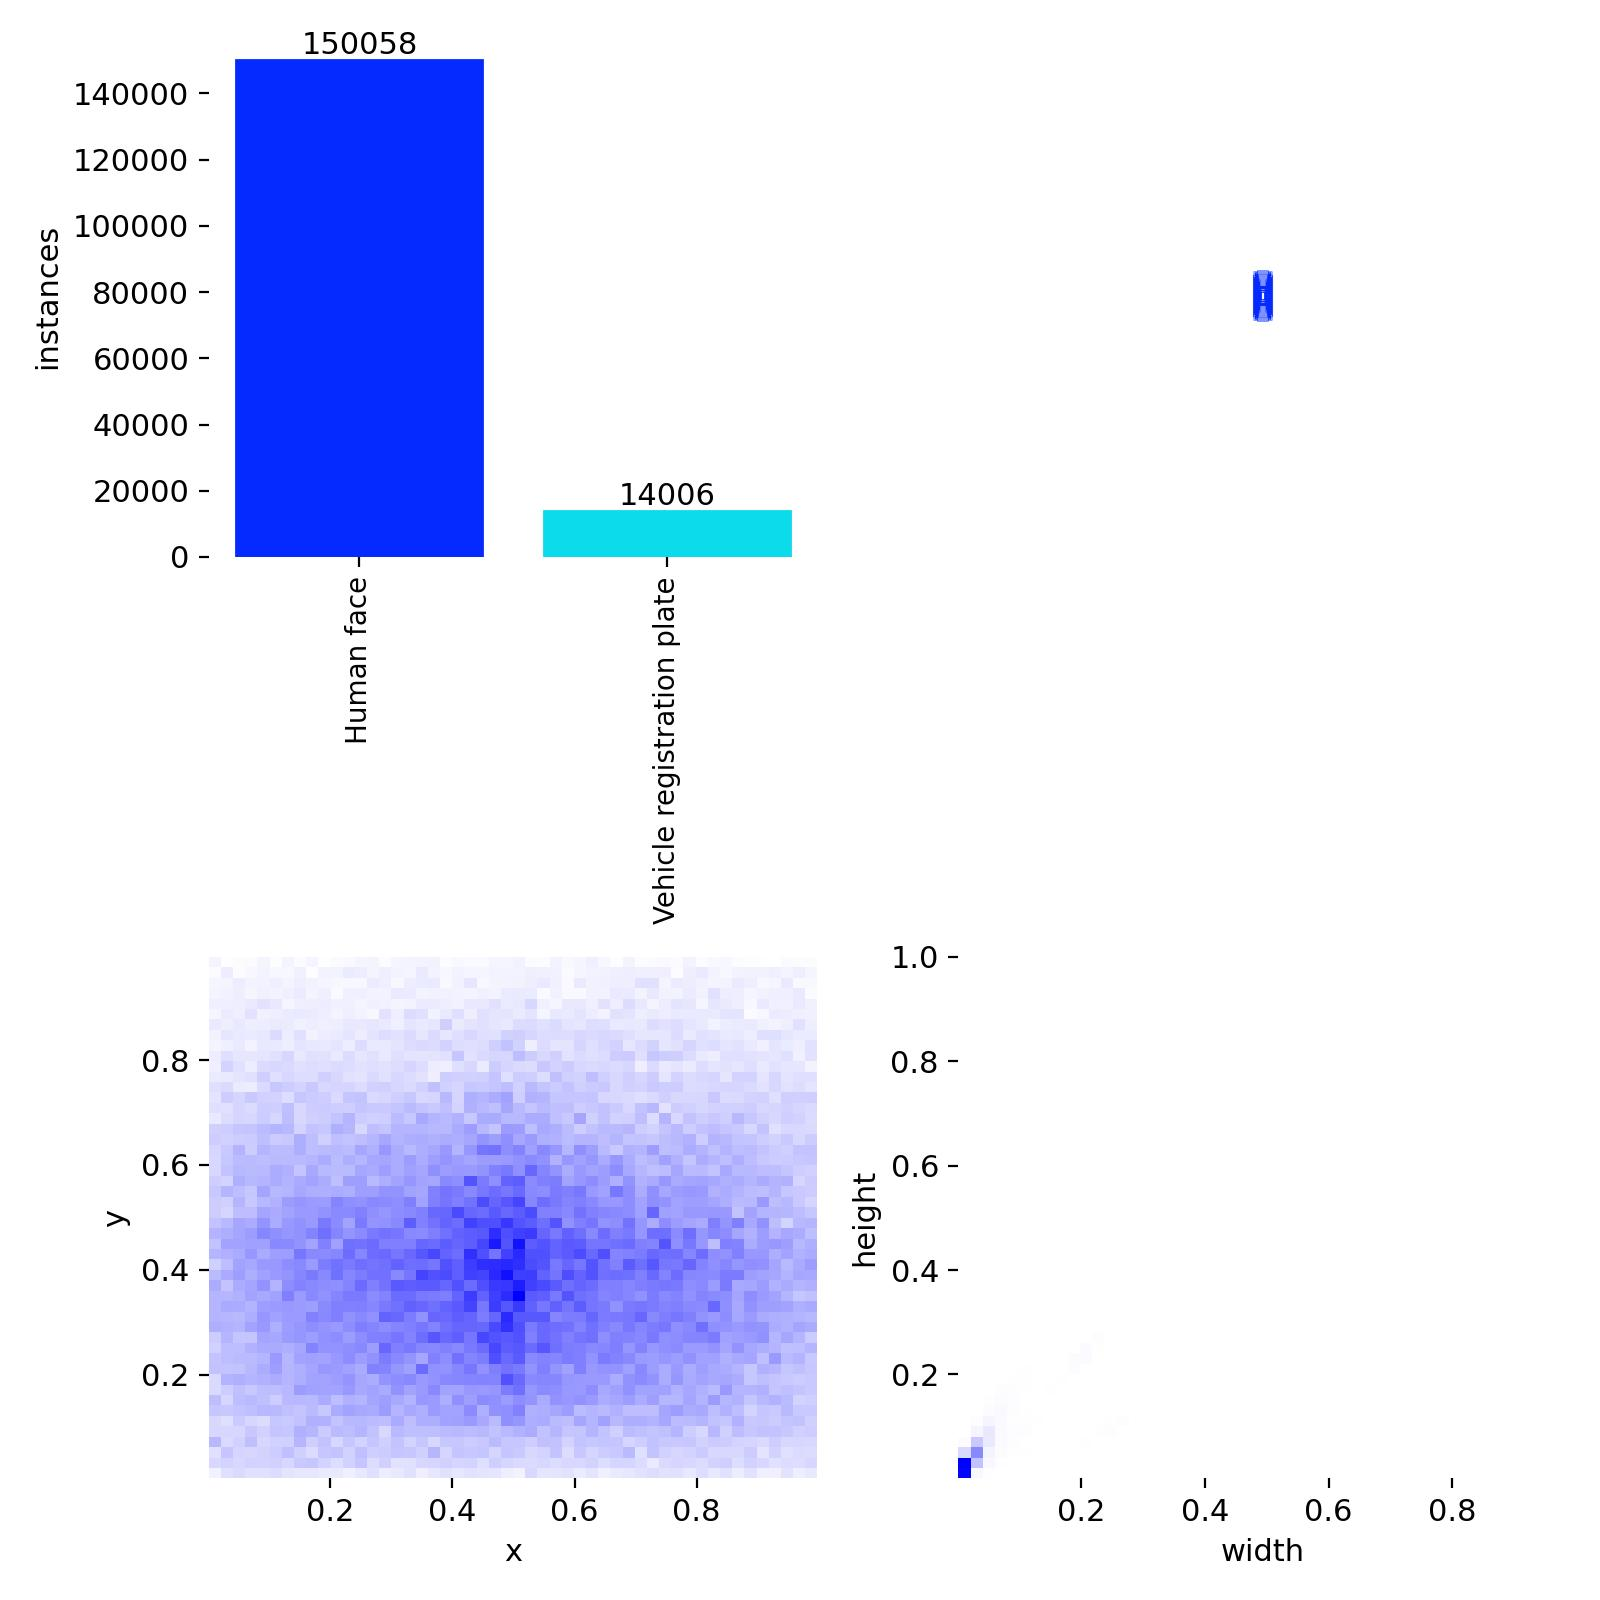
\includegraphics[width=0.72\textwidth]{figures/hinh-4-1-phan-bo-nhan.jpg}
\caption[Phân bố nhãn của tập huấn luyện]{Phân bố nhãn khi huấn luyện YOLO26s e5-dashcam: 150.058 hộp mặt và 14.006 hộp biển, tính cả ảnh được lặp lại. Phần lớn hộp rất nhỏ so với ảnh}
\label{fig:4-1}
\end{figure}

\textbf{Dữ liệu đọc biển và xác minh mặt.} Hai tập đọc biển đều cắt theo hộp nhãn nên chỉ đo khả năng đọc chữ. Tập UET do nhóm đọc bằng mắt, 40 biển dùng để chọn cách đọc và 40 biển còn lại để kiểm tra. Tập trungdinh có 767 biển, nhóm chỉ chấm 536 biển đúng định dạng Việt Nam. Với LFW, mỗi chủ thể có một hoặc ba ảnh mẫu và một ảnh kiểm tra, ảnh của những người khác đóng vai người lạ. LFW chủ yếu là mặt chính diện của người phương Tây nên chưa đại diện cho người Việt.

\textbf{Dữ liệu video.} Năm clip là video công khai trên mạng xã hội, do nhóm gán nhãn và không công bố lại. Vì chúng được dùng để tìm lỗi Engine nên có vai trò gần với tập phát triển hơn là tập kiểm thử cuối.

\subsection{Phương pháp đánh giá}

Các công thức đã nêu ở mục 2.1.2. Phần này bổ sung những quy ước ảnh hưởng đến cách đọc bảng.

\textbf{Mẫu số.} Khuôn mặt chỉ chấm trên phần WIDER (39.112 mặt), biển chỉ chấm trên phần UET (500 biển). Một dự đoán được tính đúng khi IoU từ 0,5 trở lên.

\textbf{Tiêu chí che.} Với mỗi nhãn, nhóm lấy hợp mọi hộp cùng lớp đã nới biên và kiểm tra xem có phủ từ 70\% hay không. Một hộp lệch không đủ để tính là phát hiện đúng vẫn có thể góp phần che, nên tỷ lệ đạt che thường cao hơn recall. Hộp của RedactFunnel, YuNet và EgoBlur được nới 10\% mỗi phía, hộp của deface nới 15\% theo mặc định của công cụ.

\textbf{Nhóm kích thước.} Gần một nửa số mặt của bộ đánh giá (19.153 trong 39.112) rộng dưới 16 px, rất khó nhận ra bằng mắt. Vì thế ngoài chỉ số chung, nhóm báo thêm kết quả cho mặt từ 16 px trở lên.

\textbf{Điểm vận hành.} Điểm tin cậy của hai mô hình không cùng thang đo, nên so ở cùng một ngưỡng là không công bằng. Nhóm quét 901 ngưỡng của mỗi mô hình và so tại các điểm vận hành sau:
\begin{itemize}
  \item \textbf{A:} precision mặt 0,781, dùng để so mô hình của nhóm.
  \item \textbf{B:} ngưỡng cho $F_1$ mặt cao nhất. Điểm này bỏ sót nhiều mặt hơn nên không dùng để chọn cấu hình.
  \item \textbf{C:} precision mặt 0,643, bằng precision của deface ở ngưỡng mặc định.
  \item \textbf{D:} mỗi lớp ở precision riêng, mặt 0,781 và biển từ 0,90.
\end{itemize}
Các dự đoán có điểm dưới 0,05 không được lưu.Với YOLOv8n gốc và EgoBlur, precision ở ngưỡng thấp nhất này vẫn cao hơn mục tiêu nên kết quả được ghi tại 0,05 và đánh dấu riêng.

\subsection{Hành trình huấn luyện mô hình phát hiện}

Nhóm bắt đầu từ mô hình có sẵn rồi thay đổi từng yếu tố. Bảng~\ref{tab:4-2} đặt mọi kết quả trên cùng bộ đánh giá và cùng precision mặt.

\begin{table}[!htp]
\centering\bangnho
\caption{Kết quả qua các bước huấn luyện (precision mặt 0,781)}\label{tab:4-2}
\begin{tabular}{|C{0.95cm}|L{4.3cm}|C{1.0cm}|C{1.35cm}|C{1.5cm}|C{1.5cm}|C{1.3cm}|C{1.3cm}|}
\hline
\dongdau \textbf{Bước} & \textbf{Mô hình / thử nghiệm} & \textbf{px} & \textbf{AP mặt} & \textbf{Mặt đạt che} & \textbf{Mặt $\ge$16 px} & \textbf{Biển A} & \textbf{Biển D} \\ \hline
0 & YOLOv8n gốc* & 1280 & 0,369 & 0,449 & 0,750 & 0,806 & 0,396 \\ \hline
1 & Tinh chỉnh YOLOv8n, 10 epoch & 1280 & 0,694 & 0,700 & 0,874 & 0,960 & 0,968 \\ \cline{2-8}
 & Tinh chỉnh YOLOv8n, 20 epoch & 1280 & 0,687 & 0,703 & 0,885 & 0,992 & 0,992 \\ \hline
2 & YOLO11n, 20 epoch & 1280 & 0,713 & 0,720 & 0,891 & 0,970 & 0,970 \\ \hline
3 & + nhãn giả & 1280 & 0,708 & 0,713 & 0,889 & 0,990 & 0,992 \\ \cline{2-8}
 & + ô đám đông & 1280 & 0,719 & 0,727 & 0,893 & 0,984 & 0,984 \\ \cline{2-8}
 & + lặp ảnh mặt nhỏ & 1280 & 0,717 & 0,728 & 0,901 & 0,980 & 0,980 \\ \hline
4 & YOLO11s, 12 epoch & 960 & 0,716 & 0,736 & 0,900 & 0,970 & 0,970 \\ \cline{2-8}
 & YOLO11s, 12 epoch & 1280 & 0,743 & 0,757 & 0,905 & 0,976 & 0,990 \\ \hline
5 & YOLO11n, công thức chung & 1280 & 0,741 & 0,749 & 0,897 & 0,966 & 0,972 \\ \cline{2-8}
 & YOLO26n, công thức chung & 1280 & 0,751 & 0,766 & 0,916 & 0,976 & 0,984 \\ \cline{2-8}
 & YOLO26s, công thức chung & 1280 & 0,772 & 0,792 & 0,929 & 0,958 & 0,960 \\ \hline
6 & YOLO26s + 5 epoch AdamW & 1280 & 0,776 & 0,794 & 0,930 & 0,946 & 0,950 \\ \cline{2-8}
 & Đóng băng backbone, SGD, biển $\times$2 & 1280 & 0,770 & 0,791 & 0,929 & 0,968 & 0,968 \\ \cline{2-8}
 & + 5 epoch, biển $\times$3 & 1280 & 0,773 & 0,794 & 0,930 & 0,958 & 0,974 \\ \hline
7 & Biển bị che giả & 1280 & 0,774 & 0,795 & 0,931 & 0,980 & 0,980 \\ \cline{2-8}
 & Một nửa bản sao bị che giả & 1280 & 0,777 & 0,798 & 0,932 & 0,980 & 0,980 \\ \hline
8 & \textbf{YOLO26s + dashcam (Max privacy)} & 1280 & 0,773 & 0,795 & 0,931 & 0,964 & 0,948 \\ \cline{2-8}
 & \textbf{YOLO26n + dashcam (Fast)} & 1280 & 0,748 & 0,767 & 0,913 & 0,974 & 0,970 \\ \cline{2-8}
 & YOLO26s + dashcam + mẫu âm & 1280 & 0,772 & 0,795 & 0,929 & 0,966 & 0,942 \\ \cline{2-8}
 & YOLO26n + dashcam + mẫu âm & 1280 & 0,749 & 0,767 & 0,915 & 0,974 & 0,970 \\ \hline
\end{tabular}
\par\vspace{3pt}{\noindent\small\itshape Cột Biển A và Biển D là tỷ lệ biển đạt che tại hai điểm vận hành. * Đo ở precision mặt 0,794 vì không hạ được xuống 0,781. Hai dòng in đậm là mô hình được chọn.\par}
\end{table}

\begin{figure}[!htp]
\centering
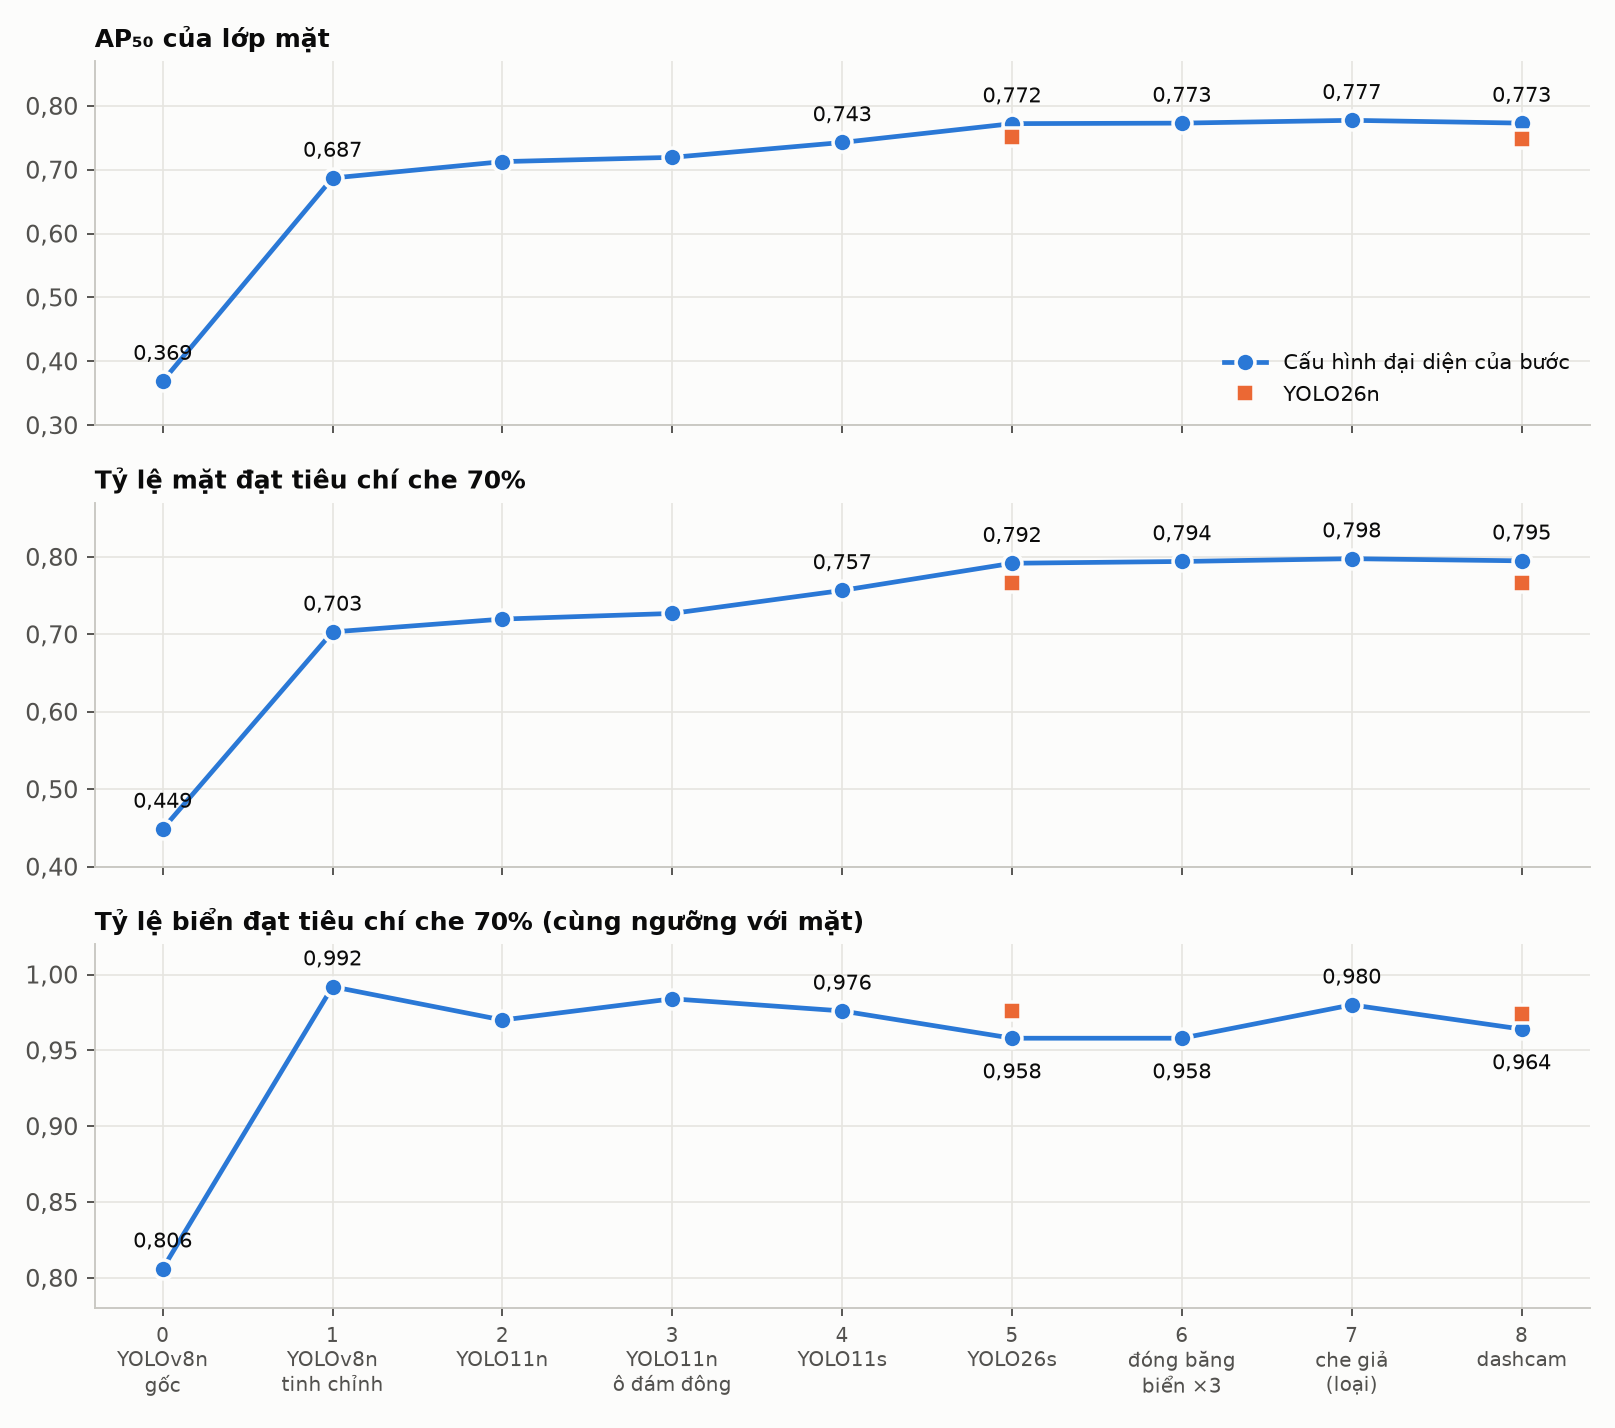
\includegraphics[width=0.8\textwidth]{figures/hinh-4-2-hanh-trinh.png}
\caption[Face AP và tỷ lệ che qua các bước huấn luyện]{Face AP và tỷ lệ che qua các bước huấn luyện, mỗi bước lấy một cấu hình đại diện. Điểm vuông là YOLO26n}
\label{fig:4-2}
\end{figure}

\textbf{Bước 0 và 1.} Mô hình gốc chỉ đạt 0,449 mặt được che. Sau 10 epoch huấn luyện trên WIDER và biển số Việt Nam, con số này lên 0,700, còn biển tăng từ 0,806 lên 0,960. Đây là bước cải thiện lớn nhất, cho thấy dữ liệu đúng bài toán quan trọng hơn mọi mẹo về sau.

\textbf{Bước 2.} YOLO11n với cùng dữ liệu tốt hơn YOLOv8n ở cả AP (0,713 so với 0,687) và tỷ lệ mặt được che (0,720 so với 0,703). Nhóm cũng thử cùng bộ trọng số ở ba kích thước đầu vào (Bảng~\ref{tab:4-3}). Chạy ở 640 px làm mất 21 điểm phần trăm, nhiều hơn hẳn lợi ích của việc đổi sang mô hình lớn hơn, vì vậy Engine mặc định dùng 1280 px.

\begin{table}[!htp]
\centering\bangfont
\caption{Độ chính xác theo kích thước đầu vào 640 / 960 / 1280}\label{tab:4-3}
\begin{tabular}{|L{2.9cm}|L{3.1cm}|C{1.2cm}|C{1.2cm}|C{1.2cm}|L{4.4cm}|}
\hline
\dongdau \textbf{Mô hình} & \textbf{Chỉ số} & \textbf{640} & \textbf{960} & \textbf{1280} & \textbf{Nhận xét} \\ \hline
YOLO11n, 20 epoch & Face AP & 0,519 & 0,650 & 0,713 & Cùng precision mặt 0,78 \\ \cline{2-6}
 & Mặt đạt che & 0,510 & 0,653 & 0,720 & Mất 6,7 điểm ở 960, 21 điểm ở 640 \\ \cline{2-6}
 & Mặt < 16 px đạt che & 0,202 & 0,427 & 0,541 & Mặt nhỏ mất nhiều nhất \\ \hline
YOLOv8n gốc & Face AP & 0,219 & 0,306 & 0,369 & Precision 0,794--0,811, chỉ so trong cùng hàng \\ \cline{2-6}
 & Mặt đạt che & 0,307 & 0,377 & 0,449 & Tăng kích thước vẫn kém mô hình đã tinh chỉnh \\ \hline
\end{tabular}
\end{table}

\textbf{Bước 3.} Nhóm thử ba mẹo về dữ liệu. Thêm nhãn giả làm kết quả giảm nhẹ (0,713) nên bị loại. Cắt ảnh đám đông thành ô đưa tỷ lệ lên 0,727 và được giữ lại. Lặp thêm ảnh mặt nhỏ chỉ tăng 0,001 trong khi AP giảm, nên cũng bỏ.

\textbf{Bước 4 và 5.} YOLO11s lúc đầu chỉ huấn luyện 12 epoch nên chưa so được công bằng. Ở bước 5 nhóm thống nhất công thức: 1280 px, 20 epoch, có ô đám đông. YOLO26n đạt 0,766 so với 0,749 của YOLO11n, còn YOLO26s đạt 0,792 nhưng tỷ lệ biển lại giảm từ 0,984 (YOLO26n) xuống 0,960. Nhóm chưa chạy lại YOLO11s với công thức này.

\textbf{Bước 6.} Để lấy lại biển số cho YOLO26s, thử nghiệm đầu tiên huấn luyện thêm bằng AdamW nhưng biển còn giảm xuống 0,950. Nhóm quay lại mô hình 20 epoch, đóng băng backbone, dùng SGD và lặp ảnh biển hai lần. AP biển tăng từ 0,963 lên 0,980 mà mặt gần như không đổi. Thêm 5 epoch với ảnh biển lặp ba lần đưa tỷ lệ biển lên 0,974. Vì ba yếu tố thay đổi cùng lúc nên nhóm không kết luận yếu tố nào quyết định.

\textbf{Bước 7.} Khi đánh giá trên video, nhóm phát hiện biển bị che một phần bị bỏ sót tới 55,7\%. Kiểm tra ngẫu nhiên 120 biển trong tập huấn luyện thì không có biển nào bị che. Nhóm dán mảnh ảnh che 25--70\% biển để tạo thêm mẫu. Trên ảnh, tỷ lệ biển tăng lên 0,980, nhưng trên video mức bỏ sót chỉ giảm xuống 52,5\%, trong khi tỷ lệ giữ đúng biển chủ xe giảm từ 87,1\% xuống 77,0\% và số khung người lạ bị giữ nhầm tăng từ 2 lên 10. Cả hai biến thể đều bị loại.

\textbf{Bước 8.} Từ mô hình của từng chế độ, nhóm huấn luyện thêm 5 epoch với 468 khung dashcam lặp bốn lần, vẫn giữ dữ liệu cũ và đóng băng backbone. Trên bộ đánh giá ảnh, mặt gần như không đổi (0,766 lên 0,767 và 0,794 lên 0,795), nhưng tỷ lệ biển ở điểm D giảm từ 0,984 xuống 0,970 (YOLO26n) và từ 0,974 xuống 0,948 (YOLO26s). Một phần do bộ đánh giá chỉ gán nhãn một biển chính mỗi ảnh: xem ngẫu nhiên 24 hộp bị tính là sai thì khoảng 18--20 hộp là biển thật của xe phía sau. Lợi ích của bước này chỉ thấy rõ trên video (mục 4.8), và đó là lý do nhóm chọn. Biến thể thêm ảnh đồng hồ xe làm mẫu âm bị loại vì với YOLO26n, tỷ lệ giữ đúng biển chủ xe trên clip dashcam 2 giảm từ 83,8\% xuống 52,9\%.

\textbf{Quá trình huấn luyện hai mô hình được chọn.} Trên tập validation, YOLO26s đạt mAP\textsubscript{50} 0,914 và YOLO26n đạt 0,903 ở epoch cuối (Hình~\ref{fig:4-3} và~\ref{fig:4-4}). Trên bộ đánh giá, mAP\textsubscript{50} của hai mô hình là 0,870 và 0,865. Hai loại số này đo trên dữ liệu khác nhau nên không đặt cạnh nhau. Tập validation không có khung dashcam nên không phản ánh lợi ích của bước 8, vì vậy nhóm dùng trọng số của epoch cuối thay vì epoch có validation cao nhất.

\begin{figure}[!htp]
\centering
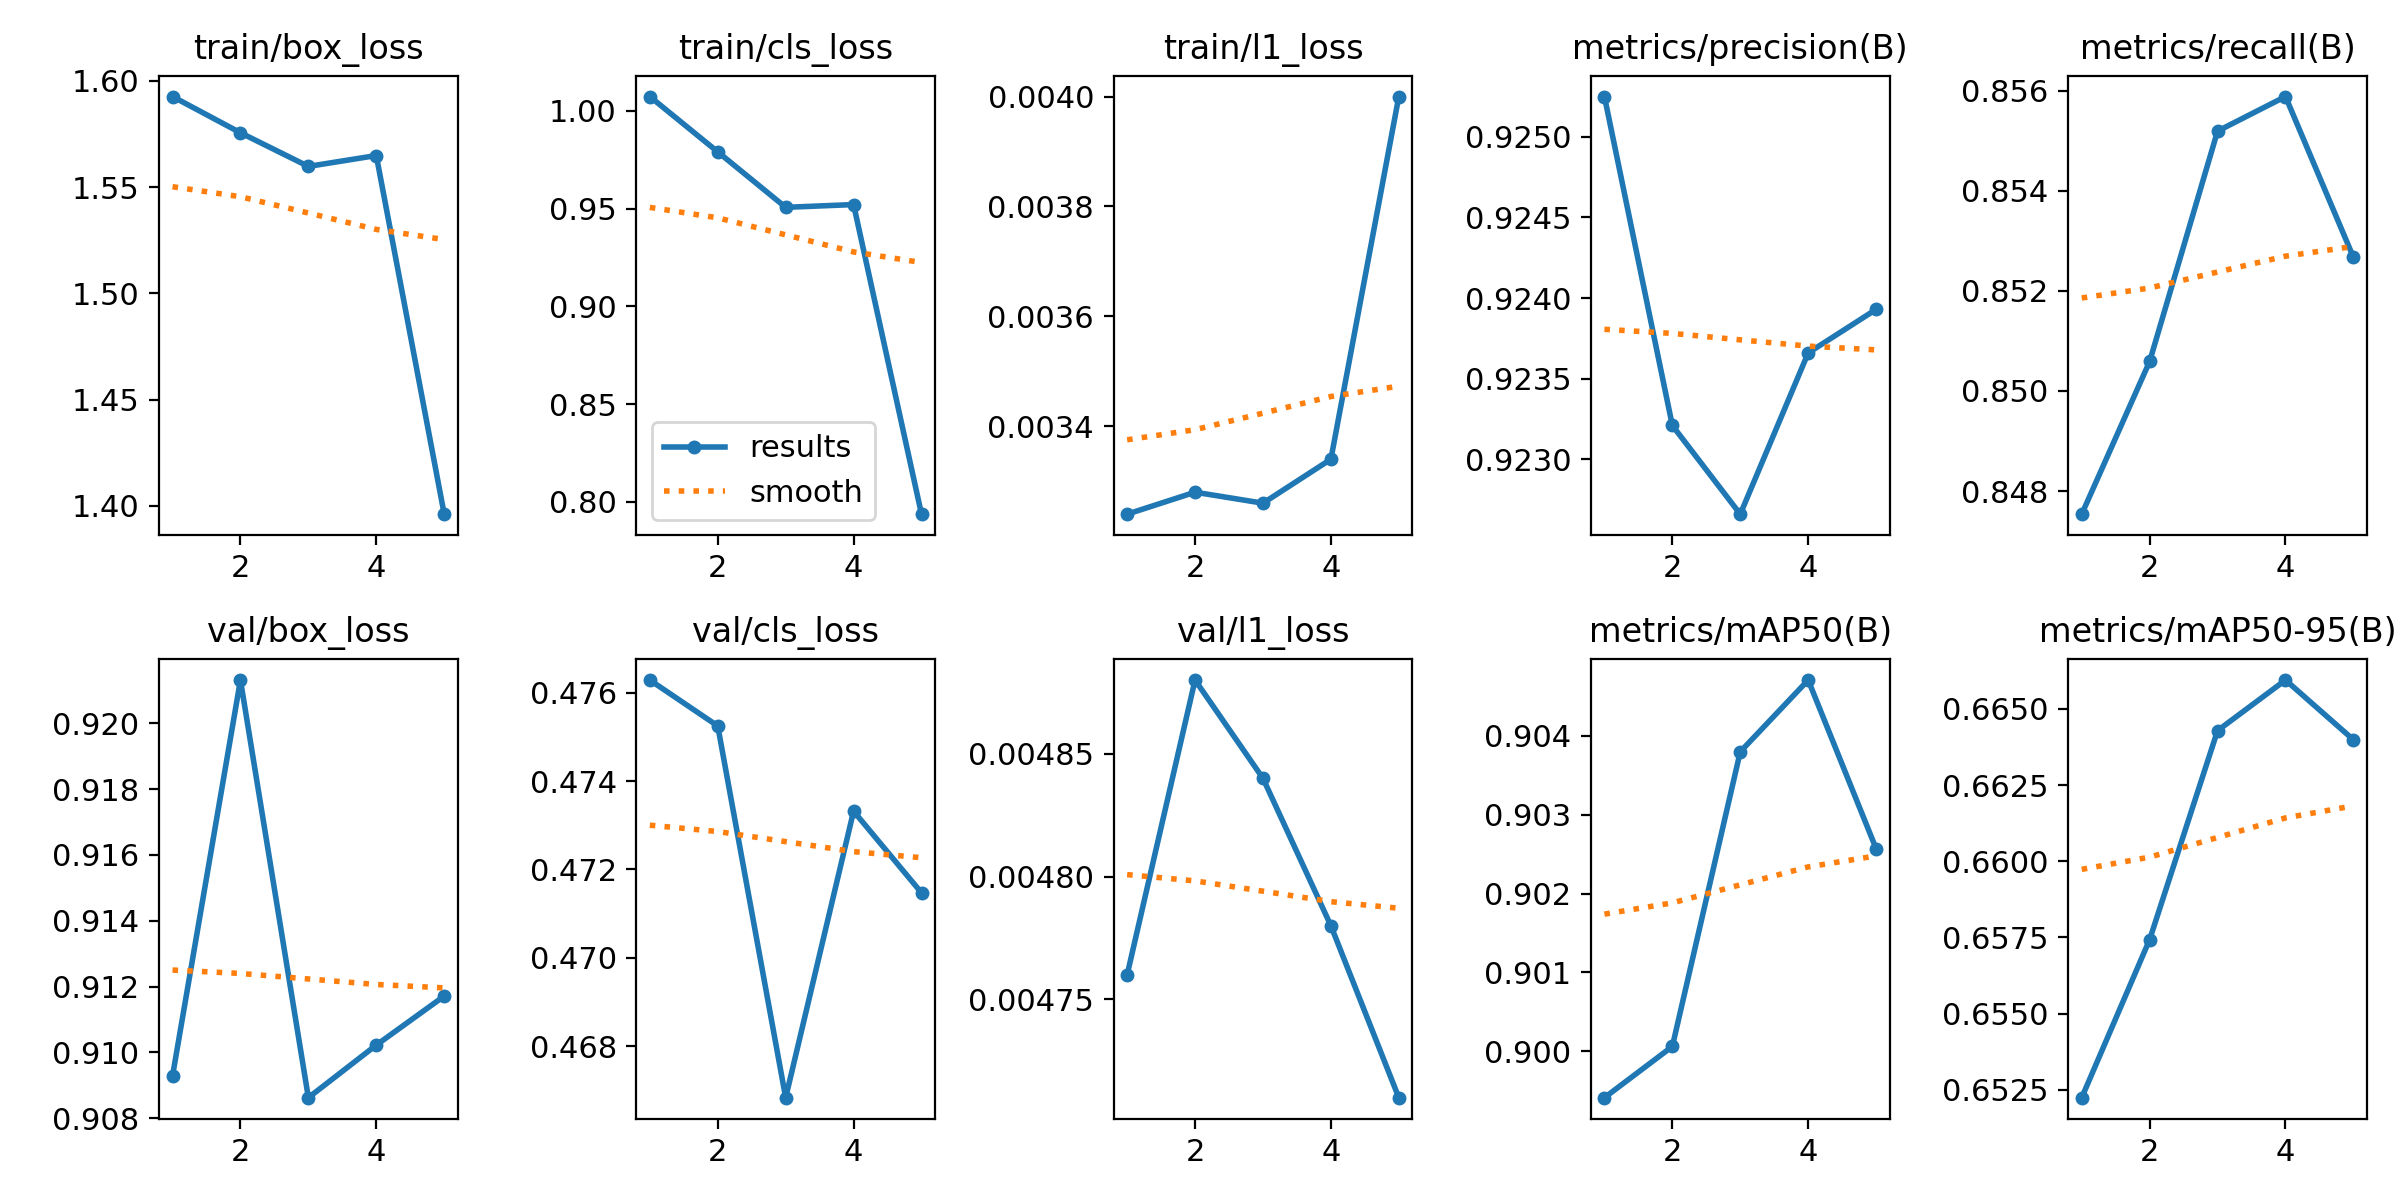
\includegraphics[width=0.98\textwidth]{figures/hinh-4-3-results-yolo26n.png}
\caption[Đường cong huấn luyện của YOLO26n (chế độ Fast)]{Đường cong huấn luyện của YOLO26n e5-dashcam (chế độ Fast), đo trên validation}
\label{fig:4-3}
\end{figure}

\begin{figure}[!htp]
\centering
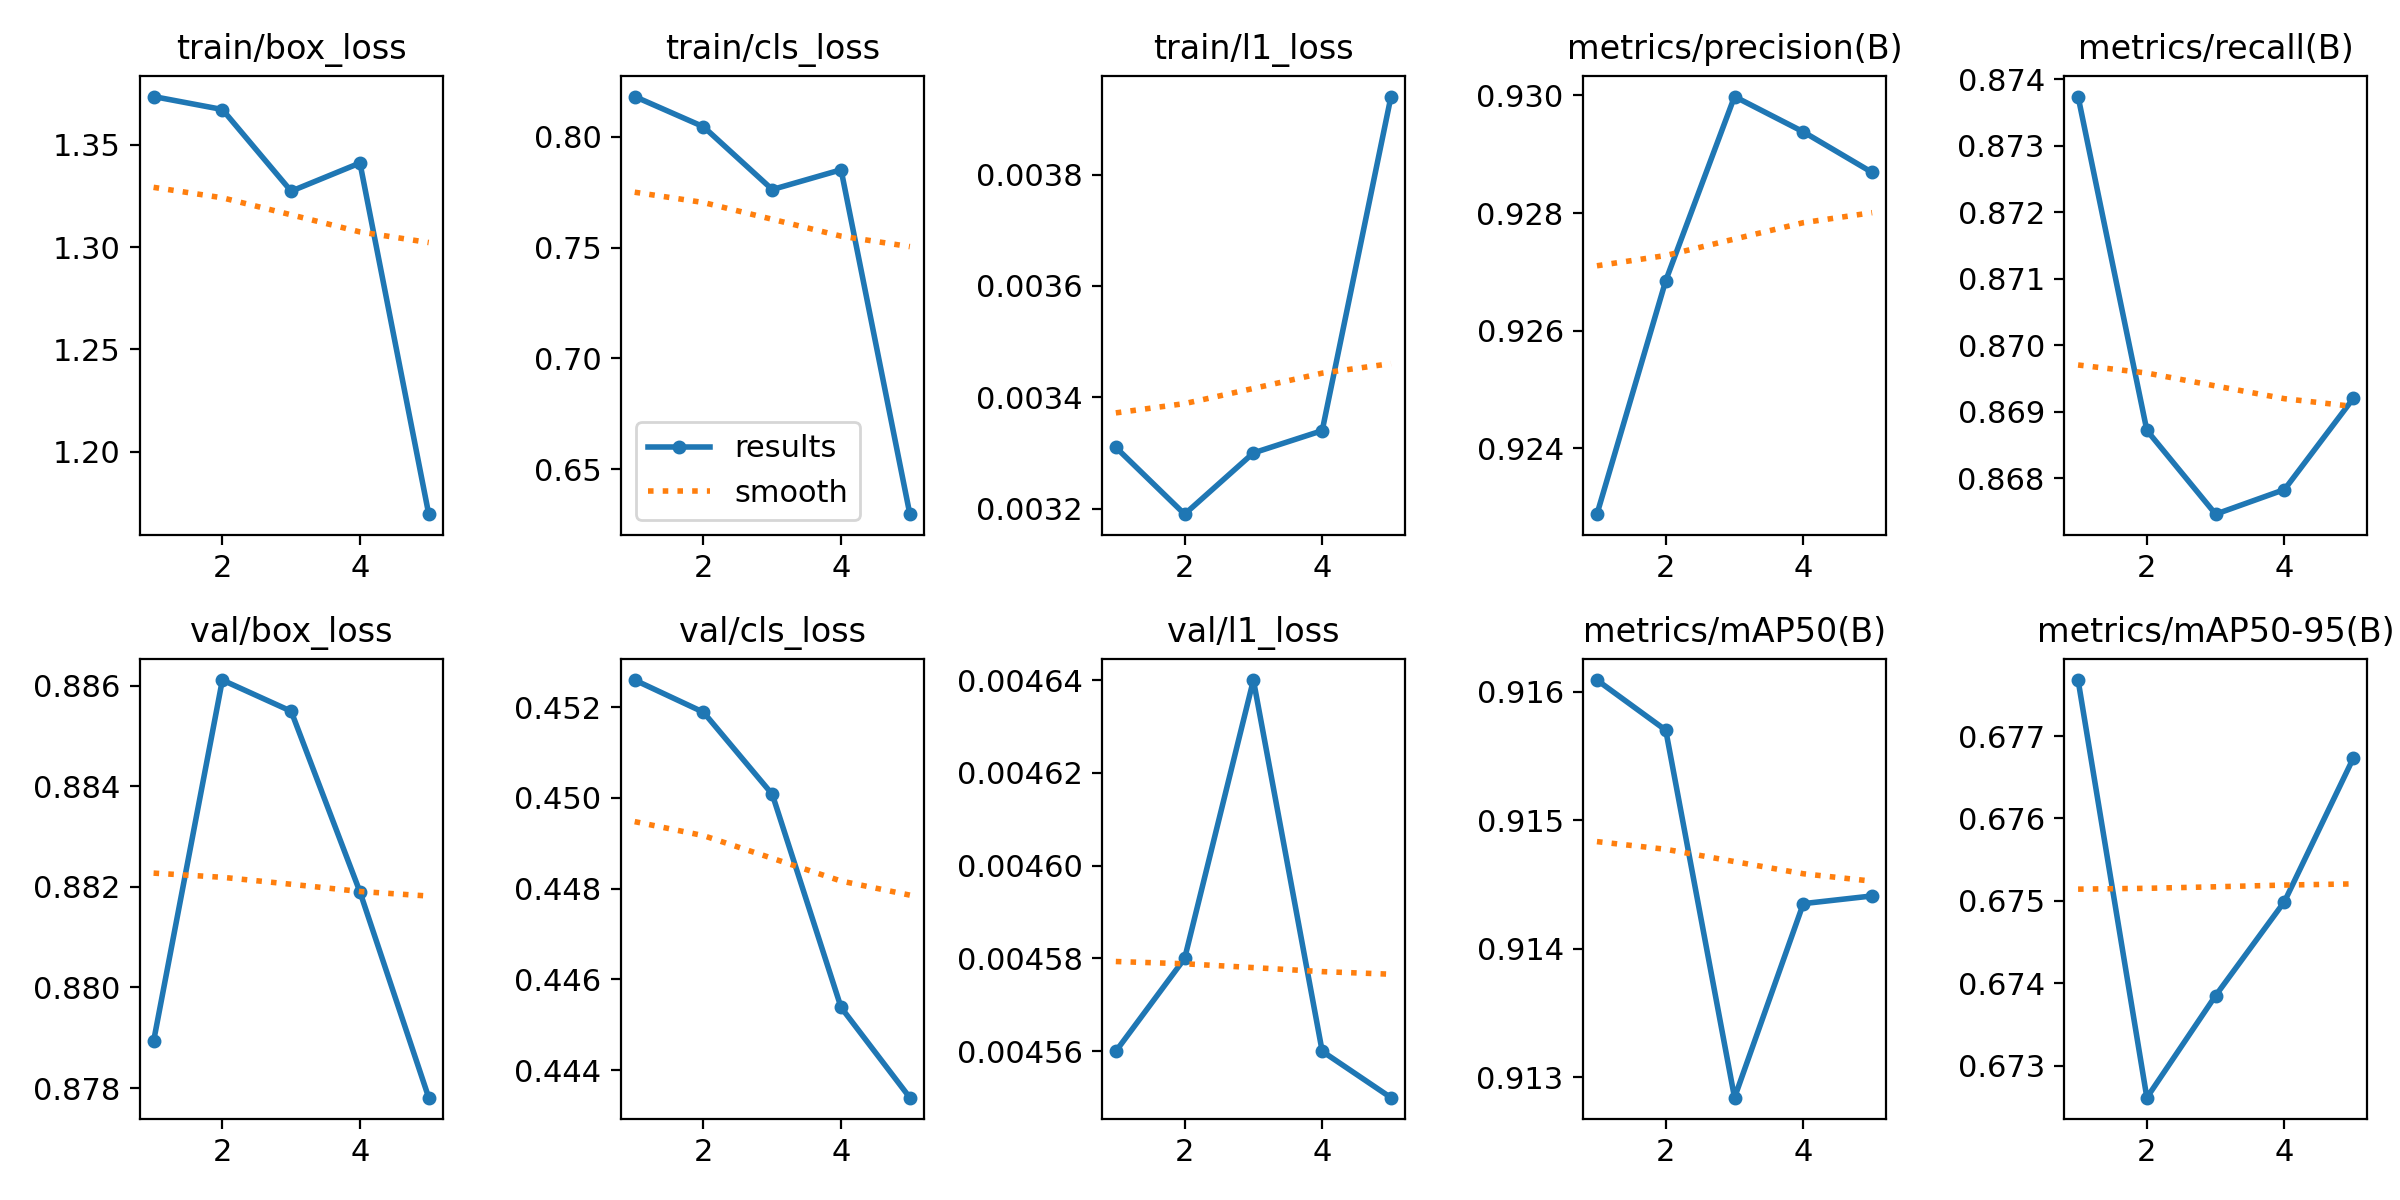
\includegraphics[width=0.98\textwidth]{figures/hinh-4-4-results-yolo26s.png}
\caption[Đường cong huấn luyện của YOLO26s (chế độ Maximum privacy)]{Đường cong huấn luyện của YOLO26s e5-dashcam (chế độ Maximum privacy), đo trên validation}
\label{fig:4-4}
\end{figure}

Hình~\ref{fig:4-5} đến~\ref{fig:4-7} cho thấy lớp biển dễ hơn lớp mặt: biển giữ $F_1$ cao trên một dải ngưỡng rộng, còn mặt giảm nhanh khi ngưỡng vượt 0,4. $F_1$ đạt đỉnh ở ngưỡng khoảng 0,31 (YOLO26n) và 0,33 (YOLO26s), nhưng Engine dùng ngưỡng thấp hơn để giảm bỏ sót. Ở ma trận nhầm lẫn, hai lớp hầu như không lẫn nhau, hộp sai chủ yếu là nền bị nhận thành mặt.

\begin{figure}[!htp]
\centering
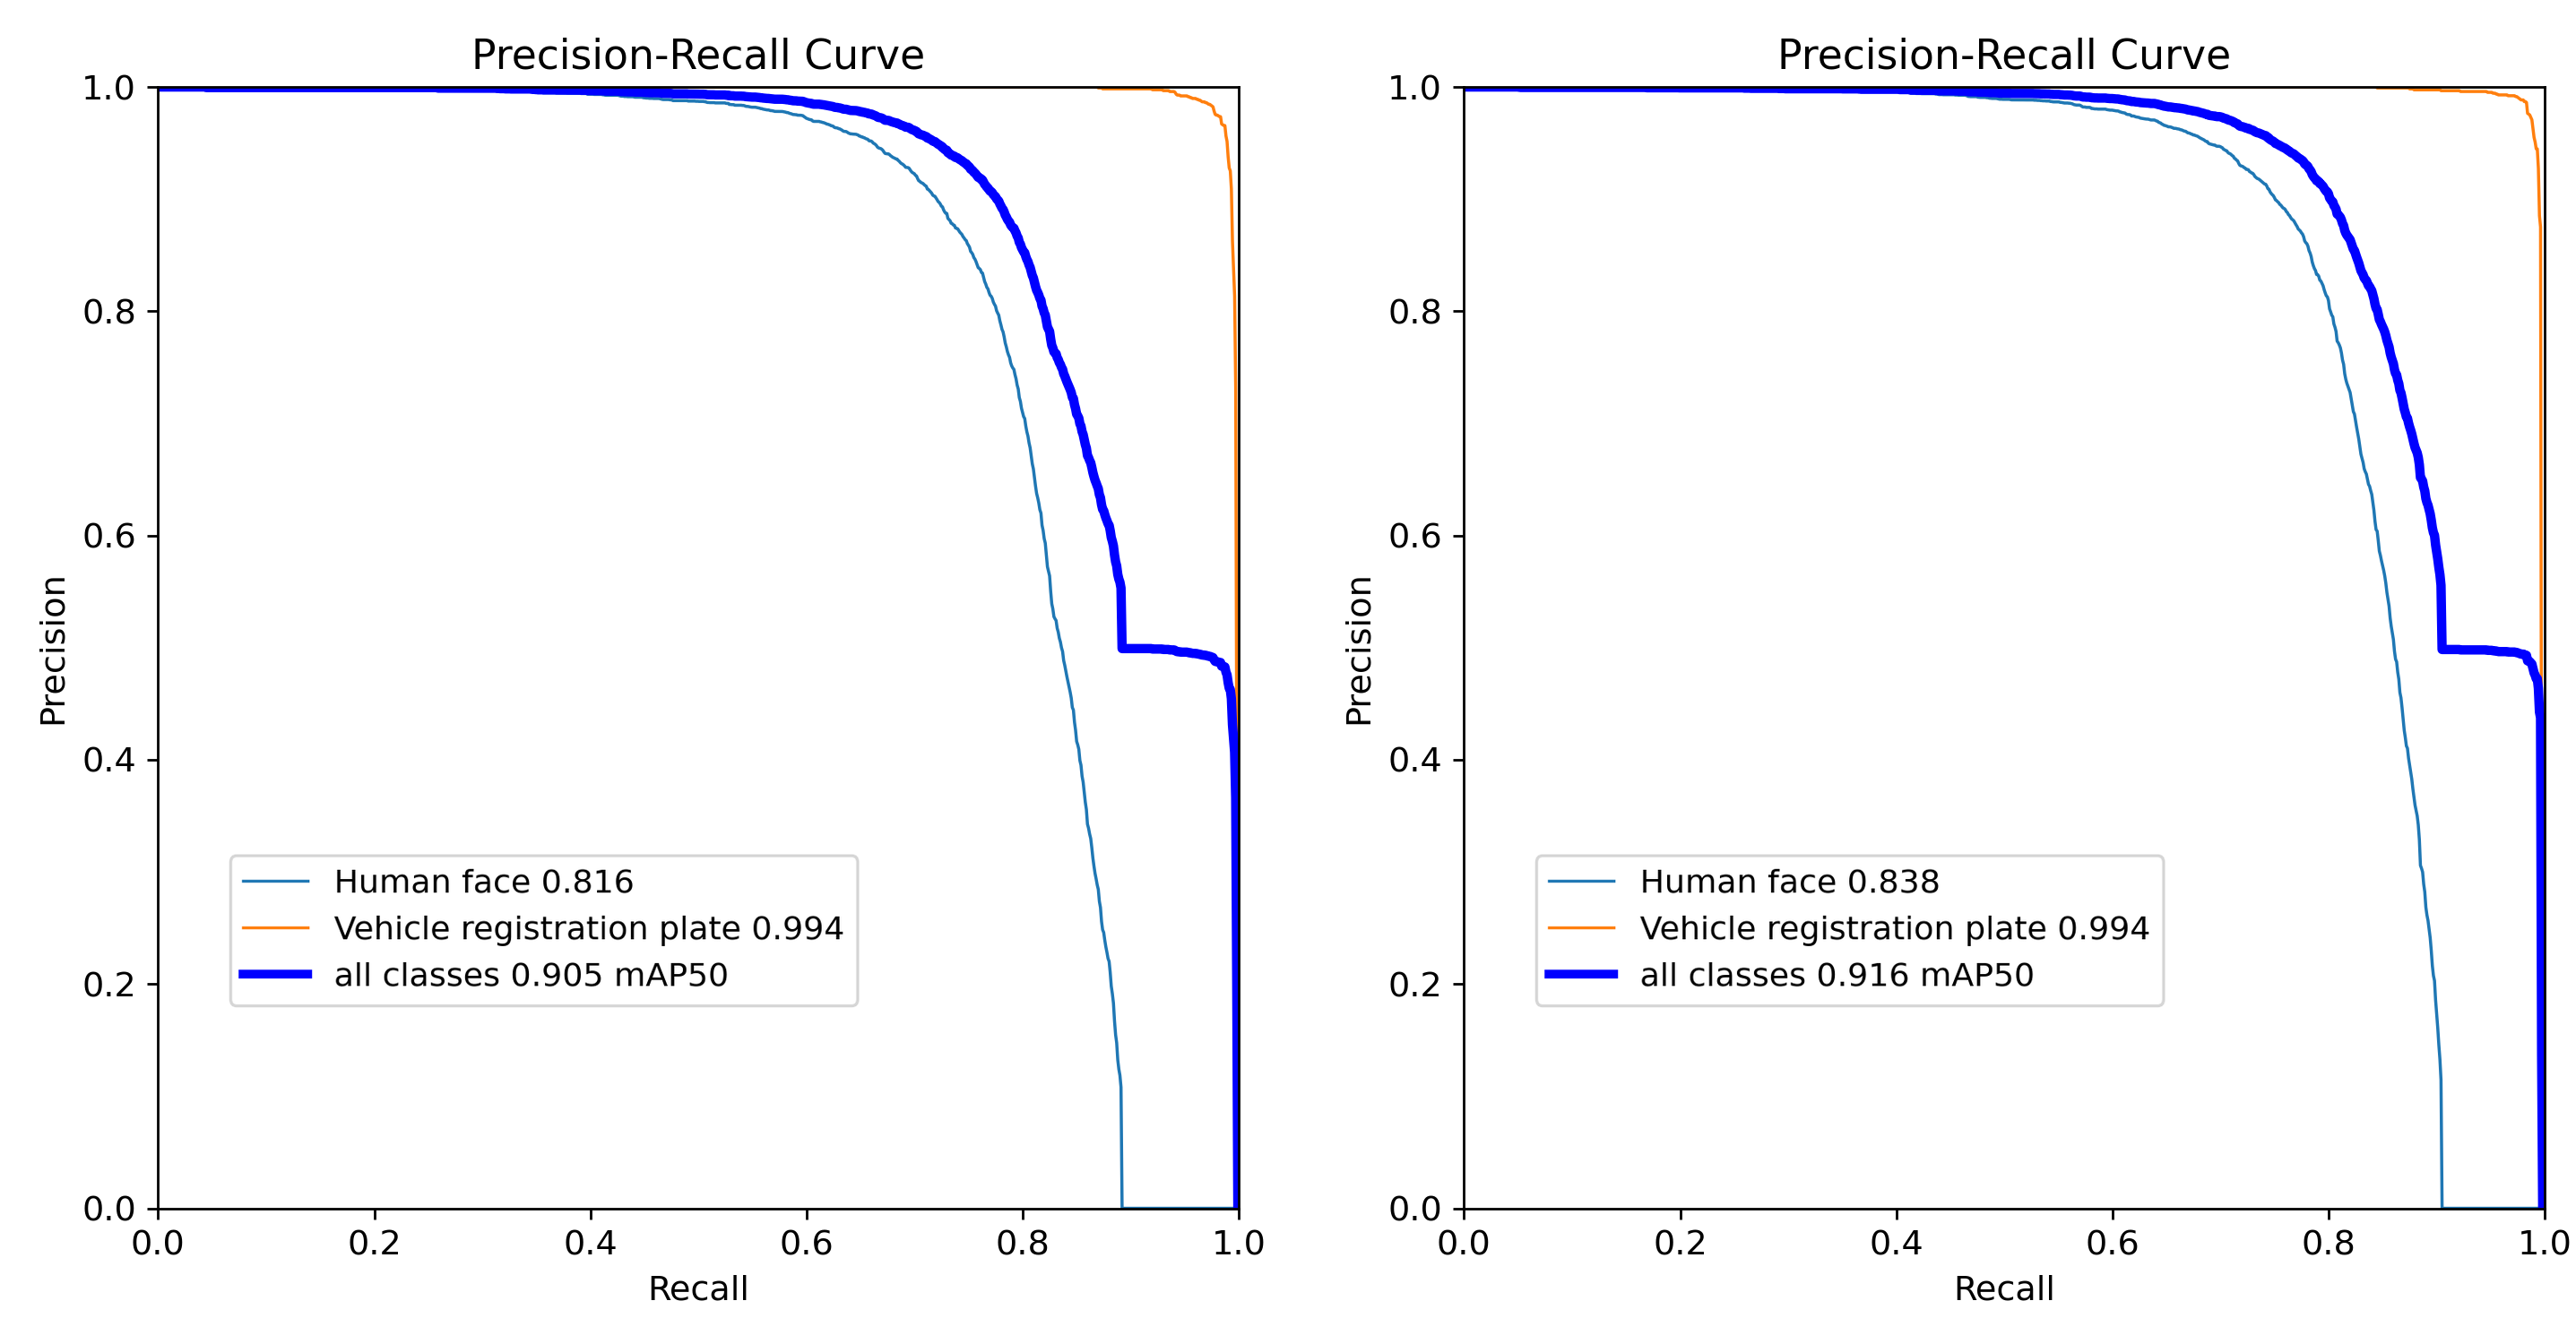
\includegraphics[width=0.98\textwidth]{figures/hinh-4-5-pr.png}
\caption[Đường cong Precision--Recall của hai mô hình được chọn]{Đường Precision--Recall của YOLO26n (trái) và YOLO26s (phải) trên validation}
\label{fig:4-5}
\end{figure}

\begin{figure}[!htp]
\centering
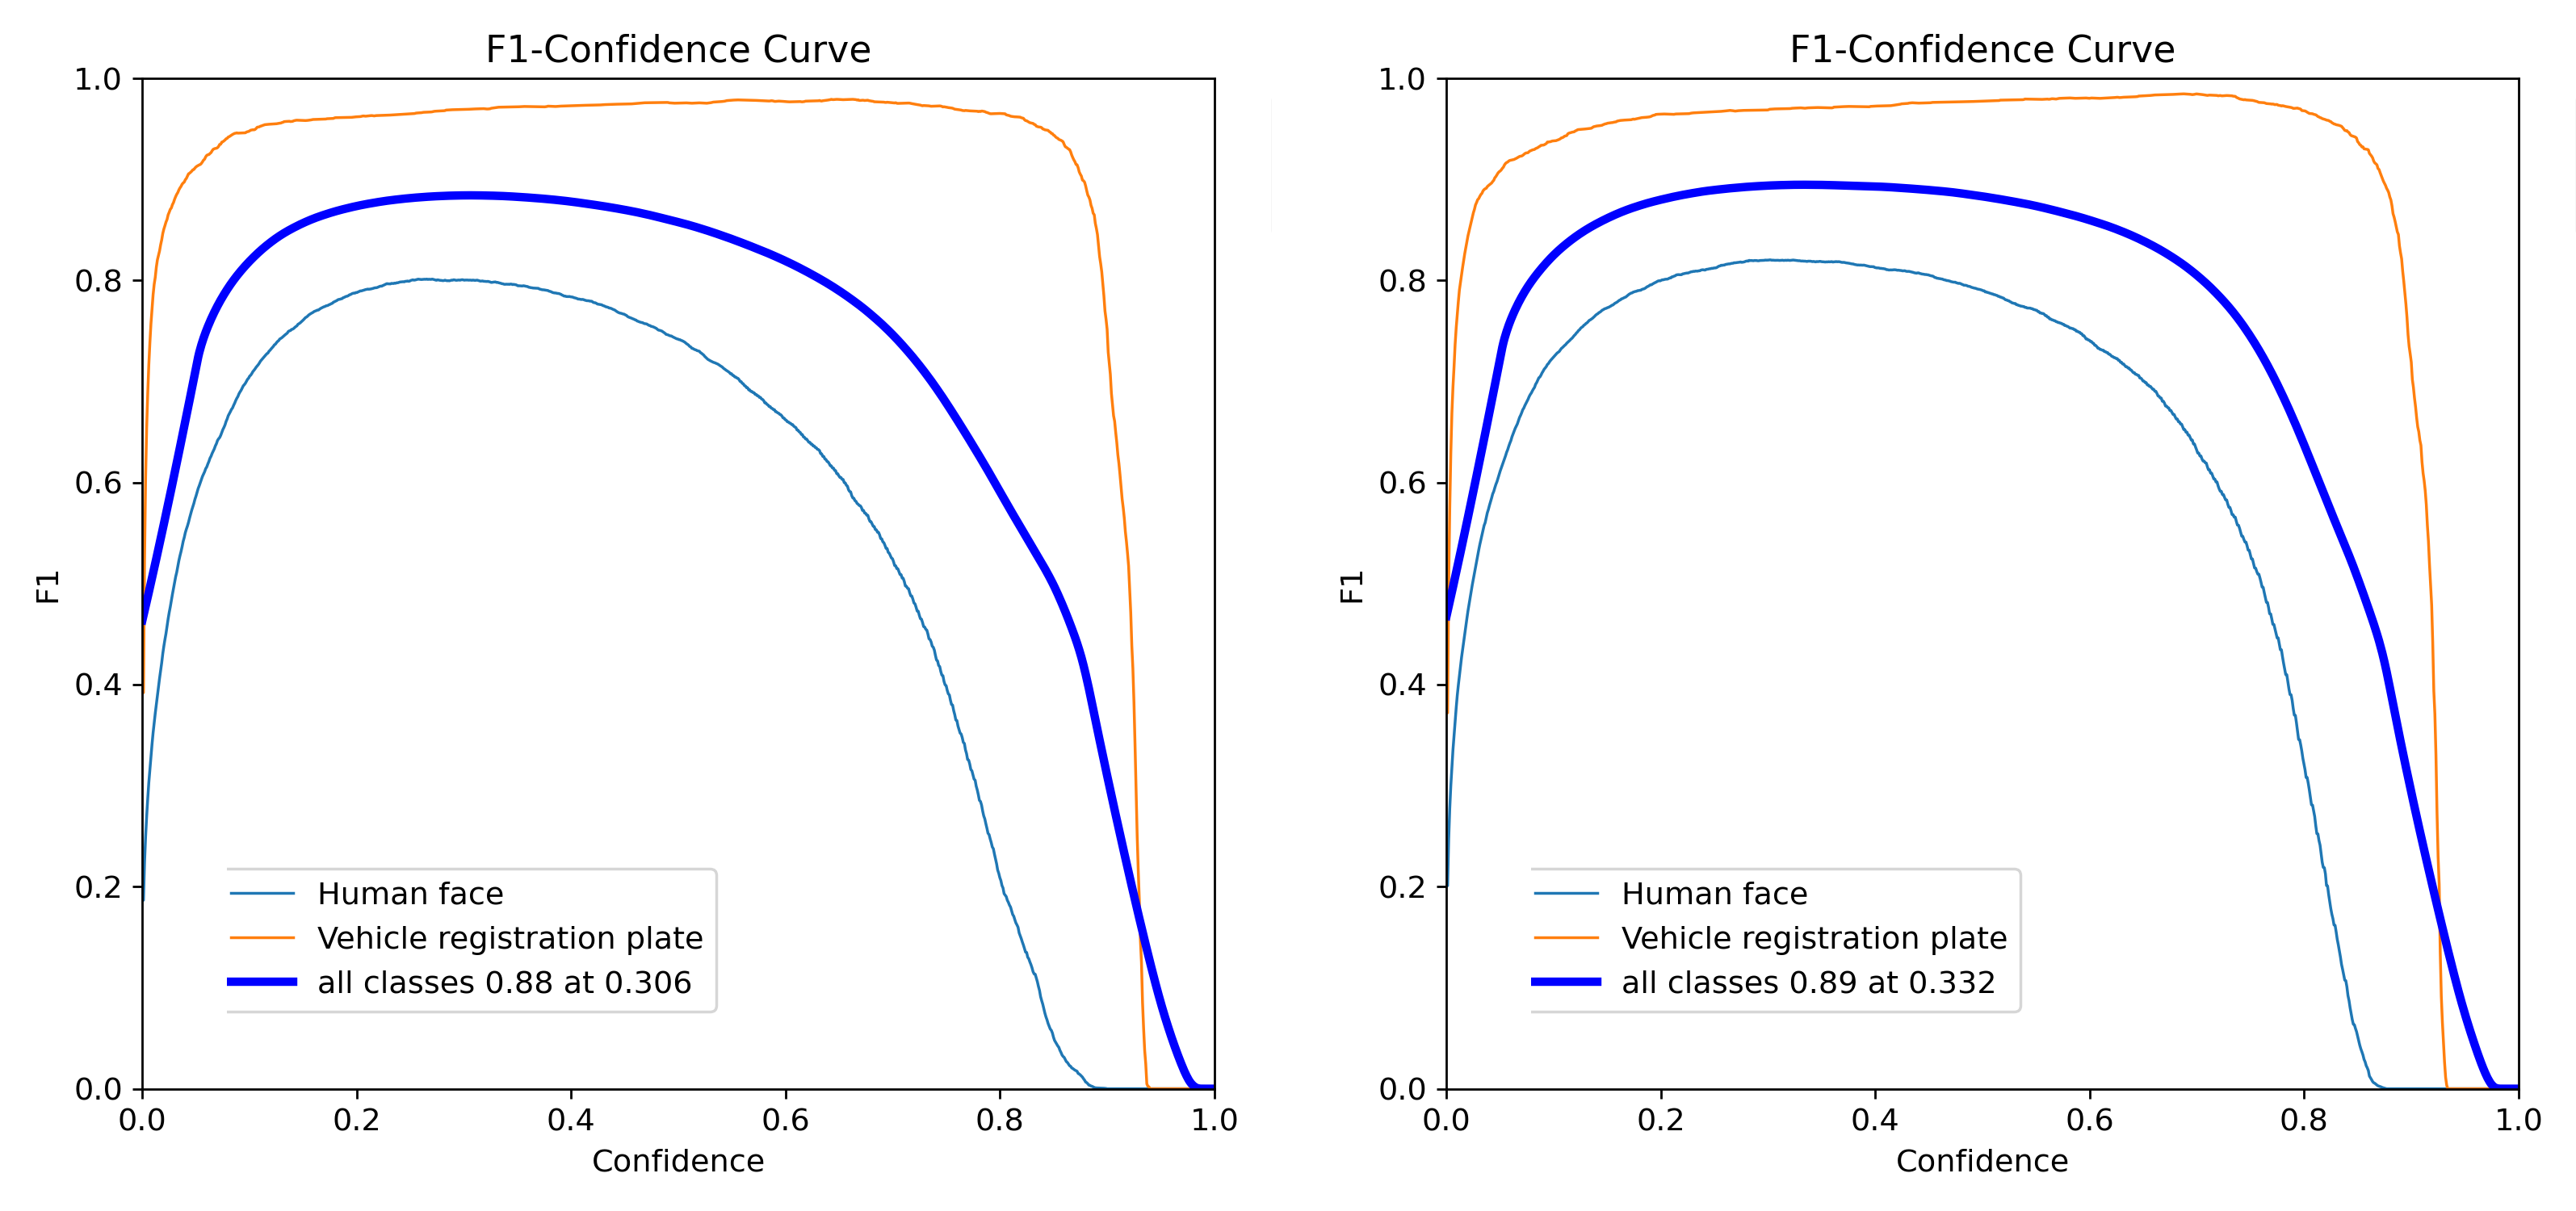
\includegraphics[width=0.98\textwidth]{figures/hinh-4-6-f1.png}
\caption[Đường cong $F_1$ theo ngưỡng tin cậy]{Đường $F_1$ theo ngưỡng tin cậy của YOLO26n (trái) và YOLO26s (phải)}
\label{fig:4-6}
\end{figure}

\begin{figure}[!htp]
\centering
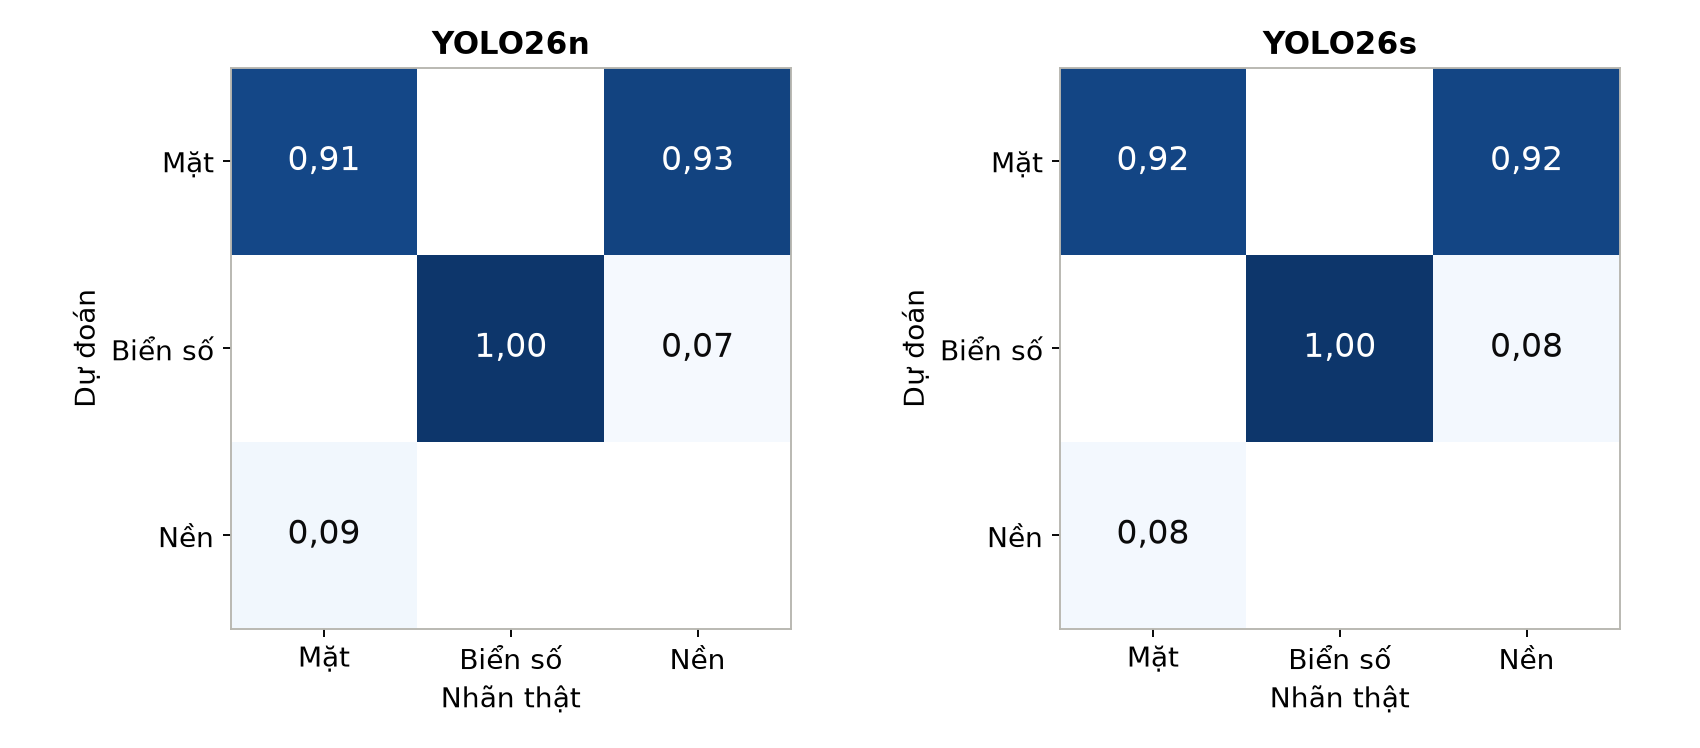
\includegraphics[width=0.98\textwidth]{figures/hinh-4-7-ma-tran.png}
\caption[Ma trận nhầm lẫn chuẩn hoá]{Ma trận nhầm lẫn chuẩn hoá của YOLO26n (trái) và YOLO26s (phải) trên validation}
\label{fig:4-7}
\end{figure}

\begin{figure}[!htp]
\centering
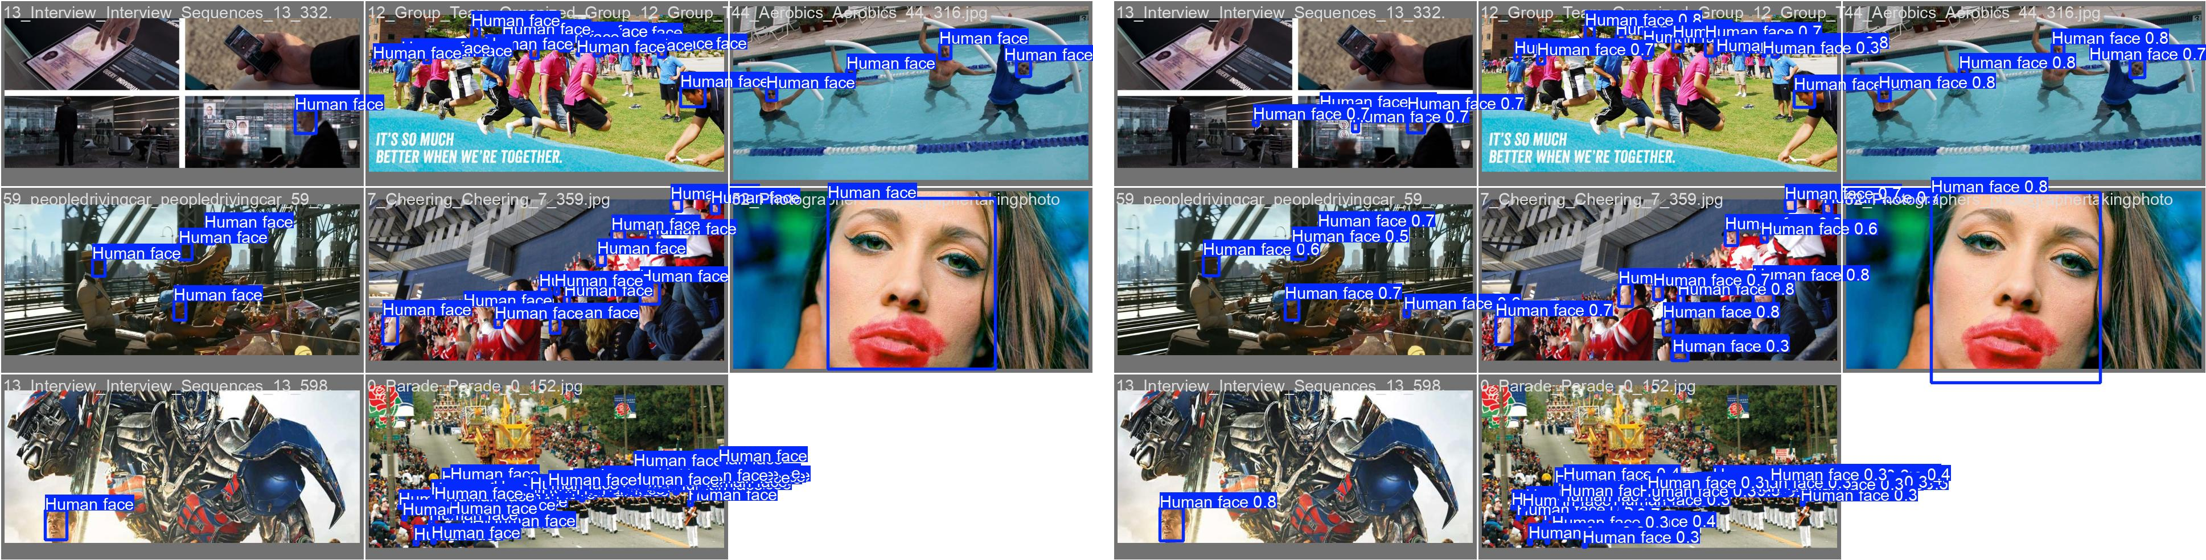
\includegraphics[width=0.98\textwidth]{figures/hinh-4-8-nhan-du-doan.png}\\[4pt]
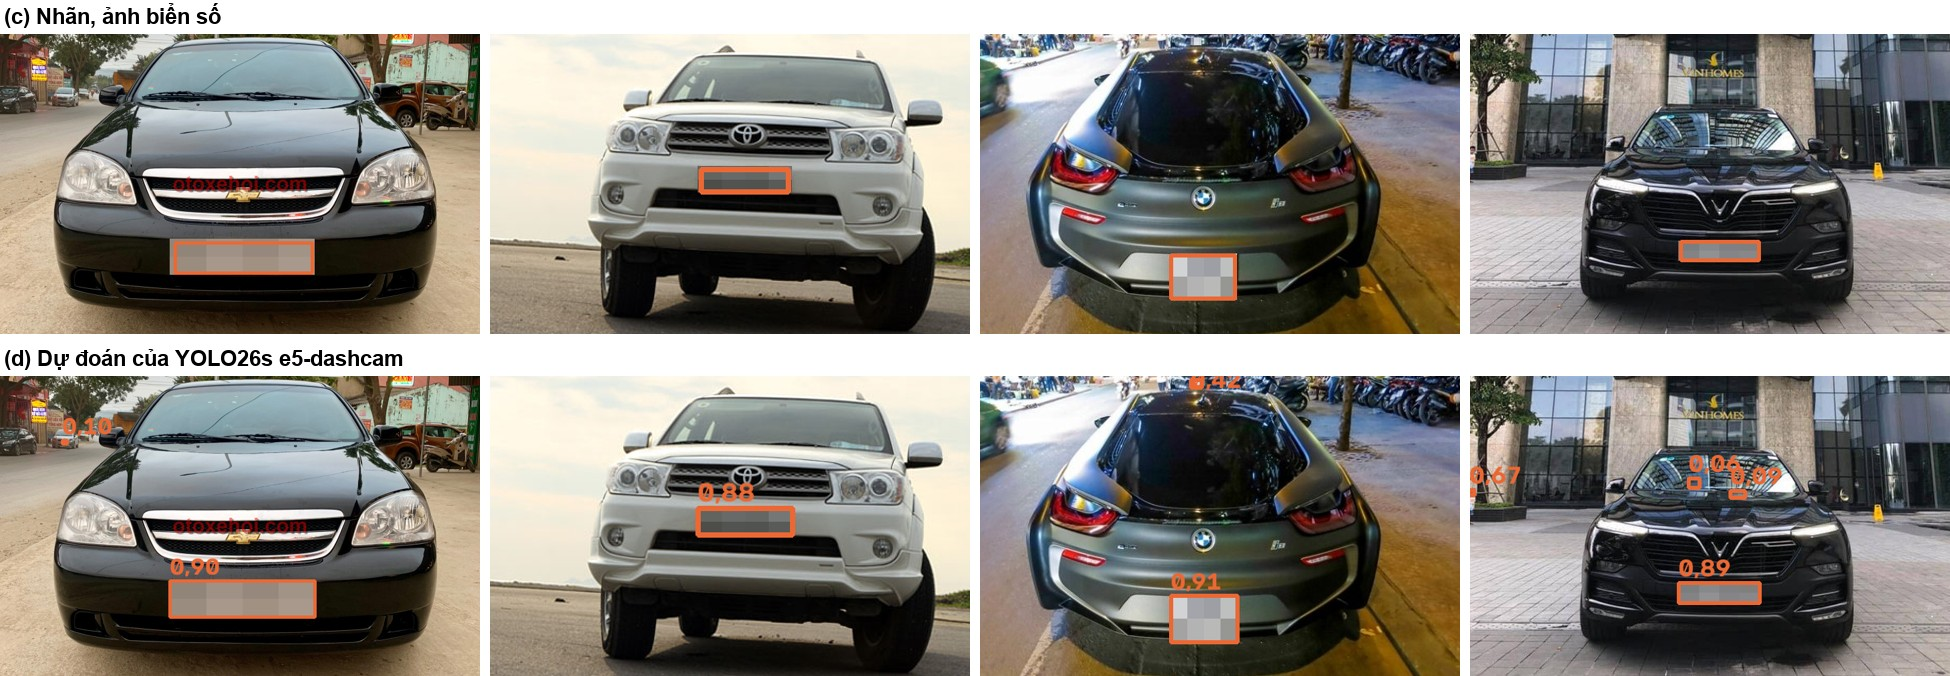
\includegraphics[width=0.98\textwidth]{figures/hinh-4-8-bien-so.jpg}
\caption[So sánh nhãn và dự đoán]{So sánh nhãn và dự đoán của YOLO26s e5-dashcam. Trên: một batch validation của WIDER FACE, trái là nhãn, phải là dự đoán. Dưới: bốn ảnh biển số của bộ đánh giá, vùng biển được làm mờ khi in}
\label{fig:4-8}
\end{figure}

\subsection{Chế độ phát hiện và ngưỡng theo từng lớp}

Người dùng chọn một trong hai chế độ. Fast dùng YOLO26n, hợp với việc duyệt nhanh. Maximum privacy dùng YOLO26s với ngưỡng thấp hơn, ưu tiên giảm bỏ sót. Bảng~\ref{tab:4-4} ghi kết quả ở đúng ngưỡng triển khai.

\begin{table}[!htp]
\centering\bangfont
\caption{Cấu hình các chế độ phát hiện}\label{tab:4-4}
\begin{tabular}{|L{6.0cm}|C{4.4cm}|C{4.4cm}|}
\hline
\dongdau & \textbf{Fast} & \textbf{Maximum privacy} \\ \hline
Mô hình & YOLO26n e5-dashcam & YOLO26s e5-dashcam \\ \hline
Kích thước đầu vào & 1280 px & 1280 px \\ \hline
Ngưỡng mặt / biển & 0,17 / 0,11 & 0,06 / 0,05 \\ \hline
Mặt: precision / recall & 0,797 / 0,726 & 0,608 / 0,797 \\ \hline
Mặt đạt che: tất cả / $\ge$16 px / <16 px & 0,761 / 0,910 / 0,606 & 0,834 / 0,950 / 0,714 \\ \hline
Biển: precision / recall & 0,747 / 0,980 & 0,643 / 0,978 \\ \hline
Số mặt không đạt che & khoảng 9.350 & khoảng 6.480 \\ \hline
Số hộp mặt sai & khoảng 7.200 & khoảng 20.100 \\ \hline
Tốc độ, GPU RTX 3050 (p50 mỗi ảnh) & 61--65 ms & 102--104 ms \\ \hline
Tốc độ, CPU i5-7200U (p50 mỗi ảnh) & 0,96--1,20 s & 2,85--2,99 s \\ \hline
Khi nào dùng & Duyệt nhanh, chấp nhận sót một số mặt nhỏ & Ưu tiên không bỏ sót, chấp nhận che nhầm nhiều hơn \\ \hline
\end{tabular}
\end{table}

\textbf{Ngưỡng riêng cho từng lớp.} Biển thường có điểm thấp hơn mặt. Với YOLO26n, nếu dùng chung ngưỡng 0,17 thì tỷ lệ biển đạt che là 0,974, còn hạ riêng ngưỡng biển xuống 0,11 thì lên 0,980, đổi lại precision biển giảm từ 0,796 xuống 0,747.

\textbf{Đánh đổi giữa hai chế độ.} Chuyển từ Fast sang Max privacy giảm khoảng 2.870 mặt không được che, chủ yếu là mặt dưới 16 px, nhưng số hộp mặt sai tăng gần ba lần. Một phần hộp sai là mặt mờ mà WIDER không gán nhãn. Với biển cận cảnh, hai chế độ gần như ngang nhau, lợi thế của Max privacy chỉ rõ trên video dashcam. Nhóm cũng thử đặt ngưỡng theo kích thước mặt: hạ ngưỡng cho mặt nhỏ tìm thêm 890 mặt nhưng kéo theo 5.619 hộp sai, nên cuối cùng chỉ giữ ngưỡng theo lớp và theo chế độ.

\subsection{So sánh với các công cụ mã nguồn mở}

Nhóm so với ba công cụ có mô hình mở: deface (dùng CenterFace, chỉ che mặt), YuNet của OpenCV (Wu và cộng sự, 2023) và EgoBlur Gen2 của Meta (Raina và cộng sự, 2023), gồm hai mô hình riêng cho mặt và biển. Bảng~\ref{tab:4-5} chỉ đặt cạnh nhau những phép đo trên cùng tập ảnh, cùng cách chấm và cùng precision mặt.

\begin{table}[!htp]
\centering\bangfont
\caption[So sánh độ chính xác với deface, YuNet, EgoBlur]{So sánh độ chính xác với deface, YuNet, EgoBlur trên bộ đánh giá 3.726 ảnh}\label{tab:4-5}
\begin{tabular}{|L{3.7cm}|C{1.6cm}|C{2.1cm}|C{2.1cm}|C{2.1cm}|C{2.1cm}|}
\hline
\dongdau \textbf{Công cụ / mô hình} & \textbf{Face AP} & \textbf{Mặt đạt che, P 0,781} & \textbf{Mặt đạt che, P 0,643} & \textbf{Mặt $\ge$16 px, P 0,781} & \textbf{Biển đạt che, P $\ge$ 0,90} \\ \hline
Max privacy (YOLO26s) & \textbf{0,773} & \textbf{0,795} & \textbf{0,828} & \textbf{0,931} & 0,948 \\ \hline
Fast (YOLO26n) & 0,748 & 0,767 & 0,803 & 0,913 & 0,970 \\ \hline
YuNet & 0,651 & 0,670 & 0,737 & 0,860 & không có \\ \hline
deface, toàn ảnh & 0,649 & 0,663 & 0,723 & 0,909 & không có \\ \hline
deface, 640$\times$480 & 0,471 & 0,490 & 0,538 & 0,825 & không có \\ \hline
EgoBlur Gen2* & 0,534 & 0,572 & --- & 0,835 & \textbf{1,000} \\ \hline
\end{tabular}
\par\vspace{3pt}{\noindent\small\itshape * Precision thấp nhất đạt được là 0,816 nên hai cột mặt của EgoBlur đo ở mức này.\par}
\end{table}

\begin{figure}[!htp]
\centering
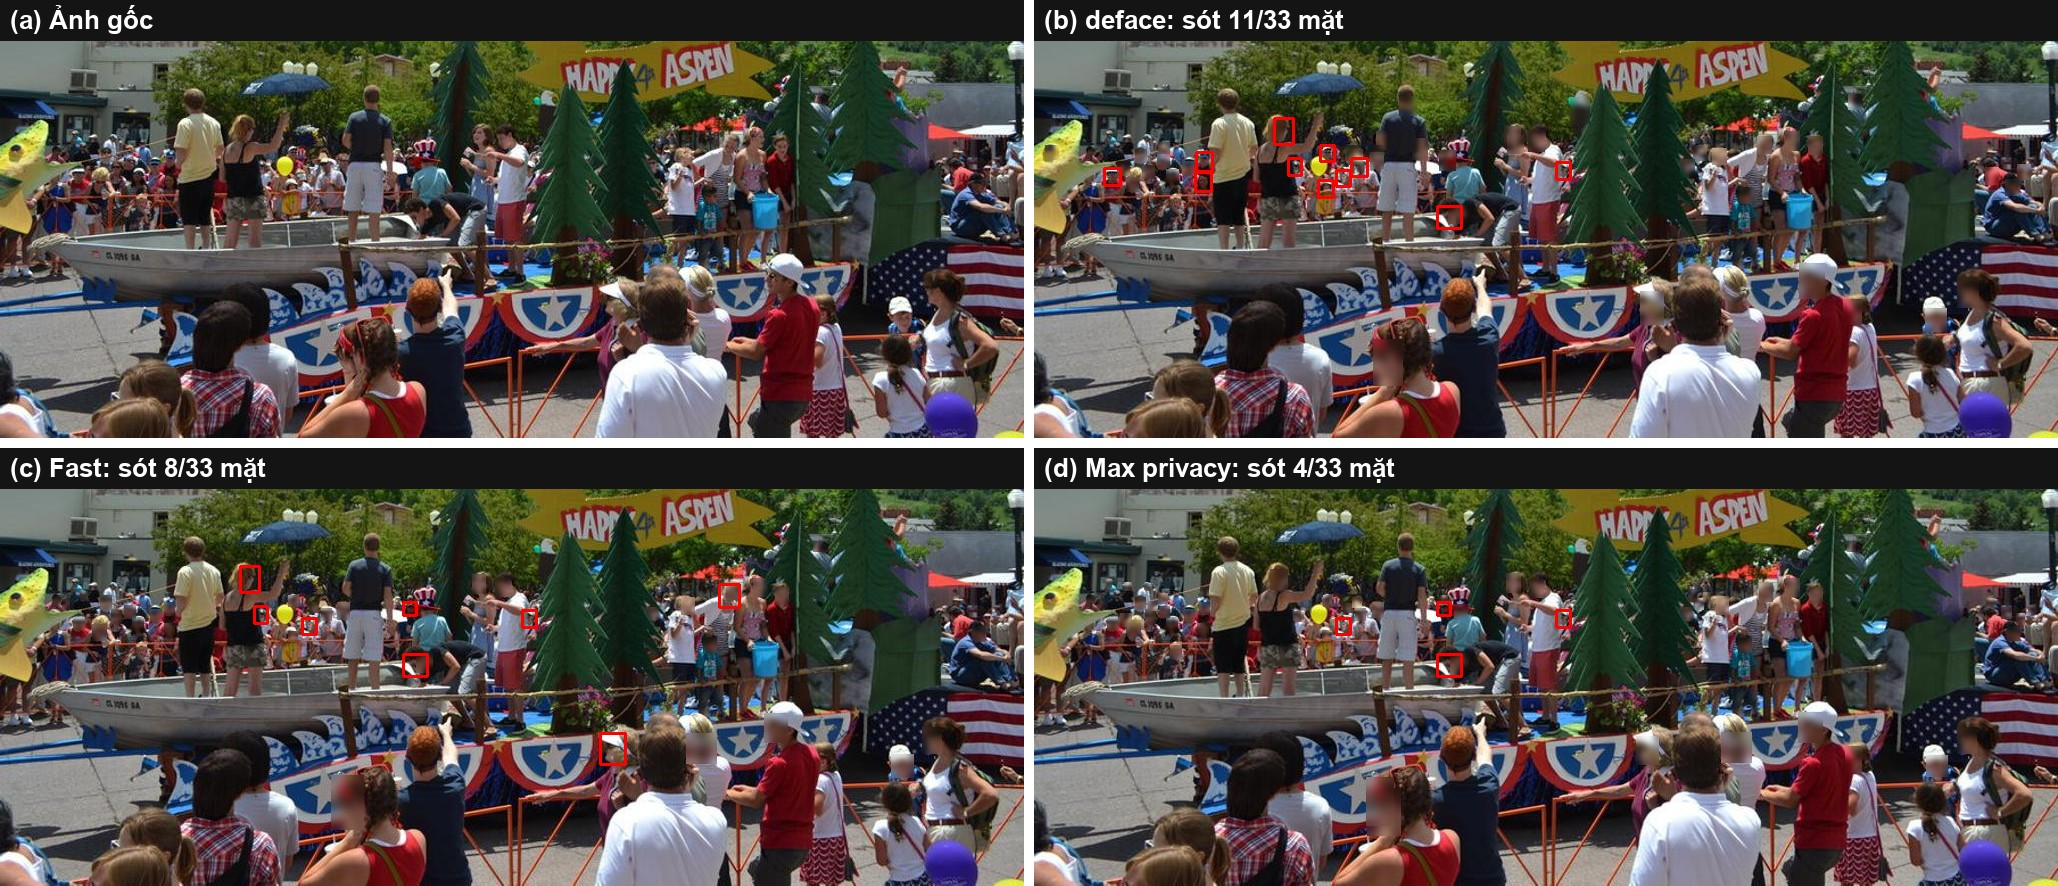
\includegraphics[width=0.98\textwidth]{figures/hinh-4-9-truc-quan.jpg}\\[4pt]
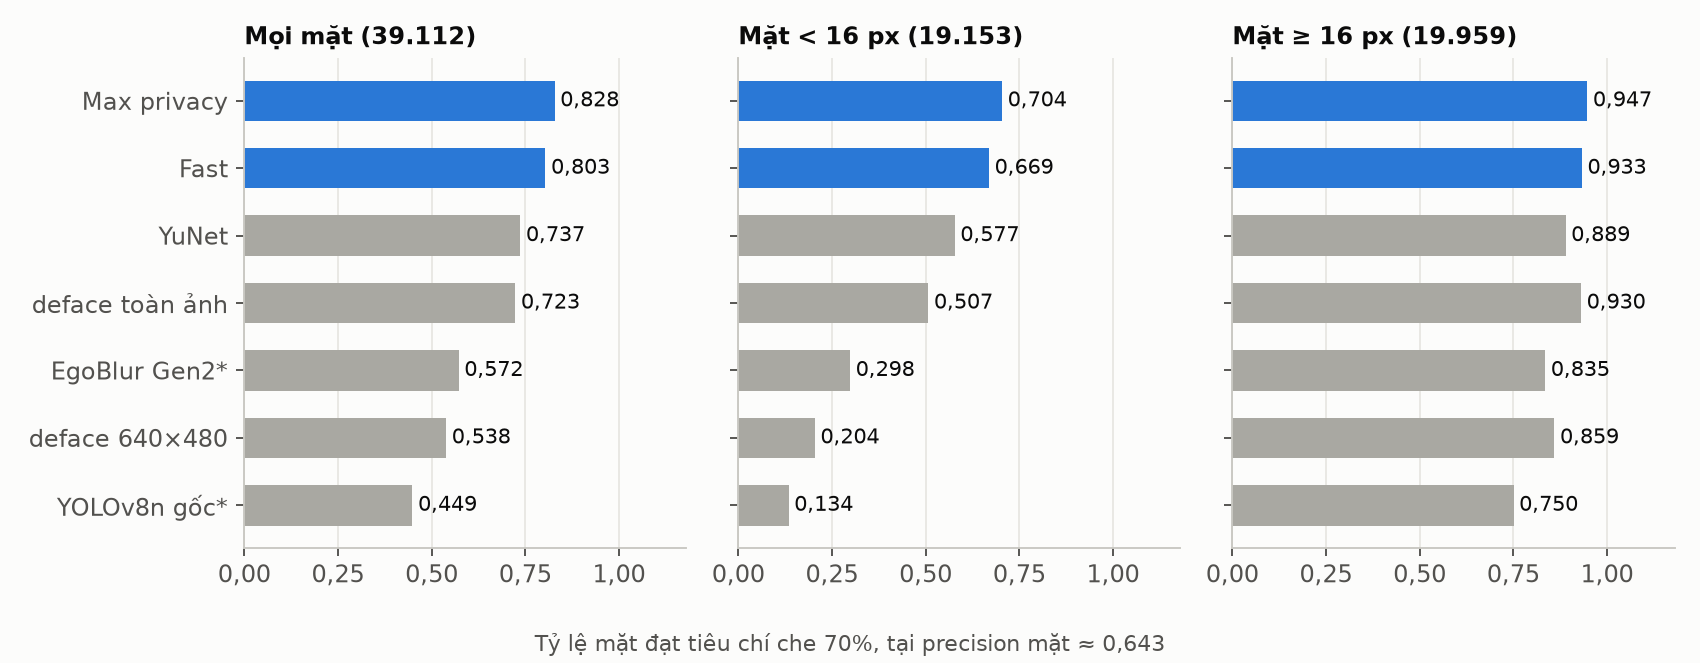
\includegraphics[width=0.85\textwidth]{figures/hinh-4-9-so-sanh-cong-cu.png}
\caption[So sánh RedactFunnel với các công cụ khác]{So sánh RedactFunnel với các công cụ khác. Trên: cùng một ảnh có 33 mặt được gán nhãn, khung đỏ là mặt chưa được che đủ 70\%. Dưới: tỷ lệ mặt đạt che ở precision 0,643. Dấu * là mô hình có precision cao hơn mức này}
\label{fig:4-9}
\end{figure}

\textbf{Khuôn mặt.} Ở đúng precision mặc định của deface (0,643), Max privacy che được 82,8\% số mặt và Fast 80,3\%, so với 72,3\% của deface. Khoảng cách chủ yếu nằm ở mặt dưới 16 px: 70,4\% và 66,9\% so với 50,7\%. Với mặt từ 16 px thì các công cụ gần nhau hơn: 94,7\%, 93,3\% và 93,0\%. Trong Hình~\ref{fig:4-9}, deface sót 11 mặt, Fast sót 8 và Max privacy sót 4. Ảnh này chỉ để minh hoạ: trên 60 ảnh đông người tương tự và ở ngưỡng mặc định của mỗi bên, deface và Fast gần bằng nhau (77,0\% và 77,3\%), còn Max privacy đạt 86,2\%.

\textbf{Biển số.} EgoBlur tìm được cả 500 biển cận cảnh, hơn cả hai chế độ của nhóm. Trên dashcam thì ngược lại: ở ngưỡng mặc định, EgoBlur bỏ sót 81,2\% biển trên clip dashcam 1, trong khi Engine với YOLO26s trước bước 8 chỉ bỏ sót 10,6\%. Hạ ngưỡng của EgoBlur xuống thấp nhất, bỏ sót còn 16,9\% nhưng chỉ che đầy đủ 30,8\% vì hộp không được nới.

\textbf{Trên cùng các clip.} Với clip điện thoại, deface khá gần Engine: trên clip 2a, tỷ lệ che đủ là 93,4\% so với 93,3\% của nhóm, nhưng deface còn bỏ sót 1,5\% mặt so với 0\%. Ở clip 1 và 2b, Engine đạt 92,1\% và 94,6\%, deface đạt 90,5\% và 85,1\%. Với mặt trong hai clip dashcam, Engine đạt 100\%, deface 80,9\% và 98,8\%, EgoBlur 51,1\% và 95,5\%. Các phép đo này dùng mô hình trước bước 8.

\textbf{Tốc độ.} deface xử lý 614 ảnh/phút trên GPU ở toàn ảnh và 294 ảnh/phút trên CPU khi chạy trực tiếp trên tệp cục bộ. Engine được đo qua cả hệ thống với ba worker: 1.646 ảnh/phút (Fast) và 1.232 ảnh/phút (Max privacy). Hai cách đo khác nhau nên không so trực tiếp. Nếu chia cho từng worker thì mỗi worker của nhóm (khoảng 550 và 410 ảnh/phút) chậm hơn một tiến trình deface.

\subsection{OCR biển số và whitelist biển số}

Để miễn che một biển số cần hai bước: đọc chuỗi và so chuỗi. Bản đầu tiên của Engine thử lần lượt PaddleOCR, EasyOCR và Tesseract, nhưng các thư viện này không được cài trong ảnh container nên luôn trả về rỗng và không biển nào được miễn che. Nhóm làm lại bước này từ đầu, so từng cách đọc trên 40 biển rồi kiểm tra trên 40 biển khác.

RapidOCR chạy đầy đủ chỉ đọc đúng 21/40 biển, EasyOCR 8/40. Vấn đề của RapidOCR nằm ở bước phát hiện chữ: nó tách một dòng thành nhiều mảnh chồng nhau nên ký tự bị lặp. Vì YOLO đã cắt sẵn biển, nhóm bỏ bước này và đọc nguyên vùng, kết quả lên 28/40 nhưng biển hai dòng thất bại. Đọc cả nguyên vùng lẫn hai nửa rồi chọn cách có điểm cao hơn đạt 37/40, kéo ngang thêm 1,3 lần thì đạt 40/40 ở cả hai nhóm biển (Hình~\ref{fig:4-10}).

\begin{figure}[!htp]
\centering
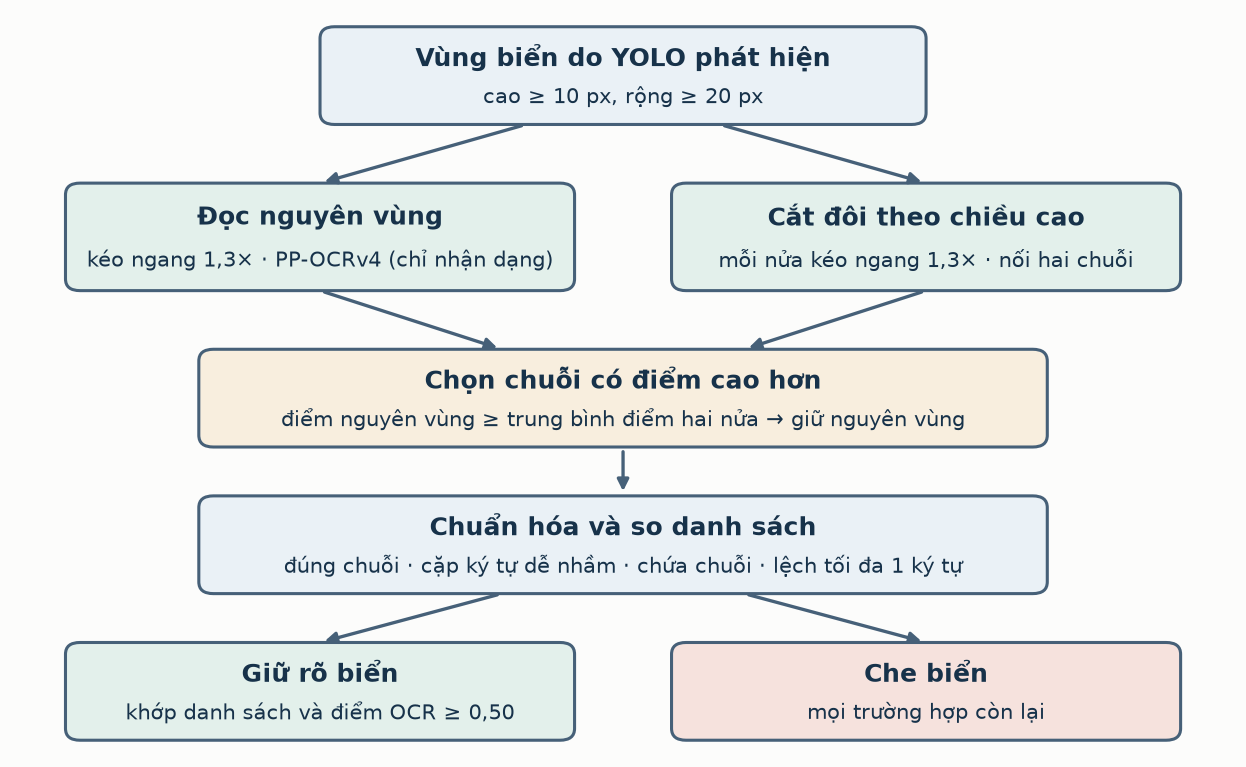
\includegraphics[width=0.8\textwidth]{figures/hinh-4-10-ocr-bien-so.png}
\caption[Quy trình đọc và so khớp biển số]{Quy trình đọc và so khớp biển số. Khi OCR lỗi hoặc không đọc được, biển mặc định bị che}
\label{fig:4-10}
\end{figure}

\begin{table}[!htp]
\centering\bangnho
\caption{So sánh các phương pháp OCR biển số}\label{tab:4-6}
\begin{tabular}{|L{4.3cm}|C{1.7cm}|C{2.0cm}|C{1.7cm}|C{2.6cm}|C{1.8cm}|}
\hline
\dongdau \textbf{Phương pháp} & \textbf{UET (80)} & \textbf{trungdinh (536)} & \textbf{2 dòng (440)} & \textbf{Thời gian / biển} & \textbf{RAM tăng thêm} \\ \hline
Tesseract & 35,0\% & 17,0\% & 12,7\% & 75 ms & 40 MB \\ \hline
RapidOCR đầy đủ & 53,8\% & 65,9\% & 79,1\% & 1.490--2.364 ms & 537 MB \\ \hline
Chỉ nhận dạng, nguyên vùng & 75,0\% & 17,5\% & 0,0\% & 45 ms & 63 MB \\ \hline
Chỉ nhận dạng, nguyên vùng hoặc chia đôi & 92,5\% & 88,1\% & 85,9\% & 120 ms & 67 MB \\ \hline
\textbf{Như trên, kéo ngang 1,3 lần (Engine)} & \textbf{100\%} & \textbf{88,6\%} & \textbf{86,6\%} & 120 ms & 66 MB \\ \hline
\end{tabular}
\end{table}

Mọi dòng trong Bảng~\ref{tab:4-6} được đo trên cùng một máy Core Ultra 5 125H giới hạn 4 luồng, chỉ dùng CPU. Tesseract đọc kém nhất trên tập UET và gần như không đọc được biển hai dòng. RapidOCR đầy đủ khá hơn nhưng chậm hơn cách của nhóm hơn 10 lần và tốn thêm khoảng 470 MB RAM. Gộp cả hai tập, Engine đọc đúng 555/616 biển (90,1\%).

Trong 61 biển đọc sai, 59 biển có hai dòng và 50 biển chỉ sai đúng một ký tự. Khoảng một phần tư số lỗi đến từ nhãn của tập dữ liệu bị thiếu ký tự. Các cặp dễ nhầm nhất là 2 với Z và 1 với 7. Tập UET chỉ có 16 biển hai dòng nên con số 100\% không có nghĩa là biển xe máy luôn đọc được.

\textbf{Quy tắc so khớp.} Vì OCR hay sai một ký tự, so chuỗi tuyệt đối sẽ che nhầm biển của chính chủ xe. Biển được miễn che khi điểm OCR từ 0,50 và thoả một trong các điều kiện: trùng chuỗi; trùng sau khi quy đổi các ký tự dễ nhầm (O và D thành 0, G thành 6, B thành 8, I thành 1, S thành 5, Z thành 2); biển trong danh sách nằm trọn trong chuỗi đọc được; hoặc cùng hai số đầu và chỉ khác tối đa một ký tự. Nhóm kiểm tra các quy tắc trên 616 biển, lần lượt coi mỗi biển là chủ xe và các biển còn lại là người lạ:

\begin{center}
\bangfont
\begin{tabular}{|L{5.0cm}|C{3.0cm}|C{3.2cm}|C{3.3cm}|}
\hline
\dongdau \textbf{Bộ so khớp} & \textbf{Giữ đúng biển chủ xe} & \textbf{Biển bị một biển khác khớp} & \textbf{Người lạ lọt, danh sách 20 biển} \\ \hline
Chỉ trùng chuỗi & 90,1\% & 0,32\% & 0,012\% \\ \hline
Bản cũ, cho sai 2--3 ký tự & 97,7\% & 46,1\% & 3,0\% \\ \hline
Cho sai tối đa 2 ký tự & 97,7\% & 7,1\% & 0,30\% \\ \hline
\textbf{Hiện tại, sai tối đa 1 ký tự} & \textbf{97,4\%} & \textbf{0,97\%} & \textbf{0,036\%} \\ \hline
\end{tabular}
\end{center}

Bản cũ cho phép sai 2--3 ký tự khiến gần một nửa số biển khớp với một biển khác. Siết xuống một ký tự chỉ mất 0,3 điểm phần trăm của chủ xe nhưng giảm tỷ lệ người lạ lọt khoảng 80 lần. Phần lọt còn lại là những cặp biển chỉ khác nhau một ký tự, không quy tắc mờ nào phân biệt được. Các biển trong tập này đều là ảnh cận cảnh, kết quả với biển nhỏ trên đường được xem ở mục 4.8.

\subsection{Whitelist khuôn mặt}

Nhóm đánh giá trên LFW với 600 chủ thể. Ảnh kiểm tra của mỗi người được so với một hoặc ba ảnh mẫu, lấy điểm cosine cao nhất. TAR là tỷ lệ ảnh của chủ thể đạt ngưỡng, tính trên 600 ảnh. FAR là tỷ lệ phép so với người khác đạt ngưỡng, tính trên 1.797.600 phép so. Kết quả ở ngưỡng 0,45 như Bảng~\ref{tab:4-7}.

\begin{table}[!htp]
\centering\bangfont
\caption[Độ chính xác whitelist khuôn mặt theo phương pháp căn chỉnh]{Độ chính xác whitelist khuôn mặt theo phương pháp căn chỉnh (ngưỡng 0,45)}\label{tab:4-7}
\begin{tabular}{|L{4.4cm}|C{1.4cm}|C{1.4cm}|C{3.3cm}|L{3.9cm}|}
\hline
\dongdau \textbf{Phương pháp} & \textbf{Ảnh mẫu} & \textbf{TAR} & \textbf{FAR (số phép so)} & \textbf{Ghi chú} \\ \hline
Hộp YOLO, không căn chỉnh & 1 & 38,8\% & $4{,}7\times10^{-5}$ (84) & Bản đầu tiên \\ \cline{2-5}
 & 3 & 64,5\% & $1{,}6\times10^{-4}$ (290) & \\ \hline
Hộp nới 15\% & 1 & 59,5\% & $1{,}5\times10^{-4}$ (273) & \\ \hline
Hộp nới 30\% & 1 & 67,8\% & $2{,}0\times10^{-3}$ (3.614) & FAR tăng khoảng 43 lần \\ \hline
Hộp nới 15\%, tô phẳng nền & 1 & 57,3\% & $4{,}8\times10^{-4}$ (865) & Nền không phải nguyên nhân \\ \hline
YuNet trên cả ảnh & 1 & 87,0\% & $3{,}9\times10^{-6}$ (7) & Mức tham khảo cao nhất \\ \cline{2-5}
 & 3 & 96,5\% & $3{,}9\times10^{-6}$ (7) & \\ \hline
\textbf{Engine, Max privacy} & 1 & \textbf{84,3\%} & $3{,}3\times10^{-6}$ (6) & YuNet trên vùng mặt \\ \cline{2-5}
 & 3 & \textbf{96,2\%} & $3{,}3\times10^{-6}$ (6) & \\ \hline
Engine, Fast & 1 & 83,5\% & $3{,}3\times10^{-6}$ (6) & \\ \cline{2-5}
 & 3 & 95,7\% & $3{,}3\times10^{-6}$ (6) & \\ \hline
\end{tabular}
\end{table}

Căn chỉnh bằng YuNet là thay đổi có tác dụng lớn nhất: với một ảnh mẫu, TAR tăng từ 38,8\% lên 84,3\% trong khi số phép so nhầm giảm từ 84 xuống 6. Nới hộp cũng tăng TAR nhưng kéo FAR tăng theo, nên bị loại. Đổi bộ phát hiện gần như không ảnh hưởng: sáu mô hình lệch nhau nhiều nhất 2 điểm phần trăm. Hình~\ref{fig:4-11} cho thấy hai phân bố tách nhau khá rõ quanh ngưỡng 0,45, và các mặt nằm trong vùng $\pm0{,}05$ được đưa vào mục cần xem lại.

\begin{figure}[!htp]
\centering
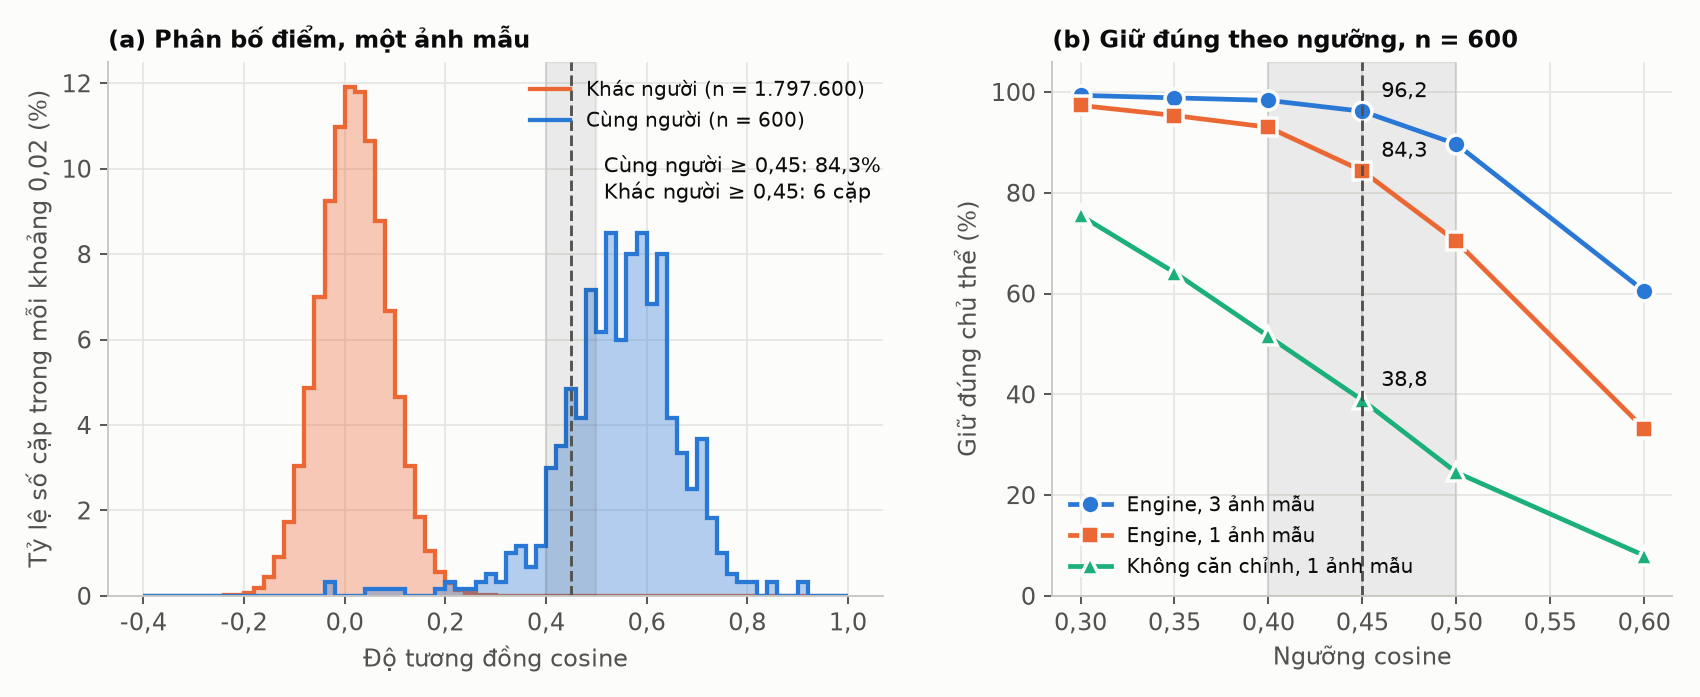
\includegraphics[width=0.98\textwidth]{figures/hinh-4-11-nguong-cosine.png}
\caption[Phân bố cosine similarity của cặp cùng người và khác người]{(a) Phân bố cosine similarity của cặp cùng người và khác người, một ảnh mẫu. (b) Tỷ lệ giữ đúng chủ thể theo ngưỡng. Vạch đứt là ngưỡng 0,45, vùng xám là vùng cần xem lại}
\label{fig:4-11}
\end{figure}

\textbf{Kích thước khuôn mặt.} Mặt càng nhỏ càng khó giữ đúng chủ thể. Với một ảnh mẫu, TAR giảm từ 84,3\% xuống 64,0\% ở 64 px, 34,7\% ở 40 px và 6,0\% ở 24 px. Dùng ba ảnh mẫu thì các mức là 96,2\%, 86,5\%, 59,3\% và 17,0\%. Nếu chấp nhận mức người lạ 1/10.000, ngưỡng ở 40 px có thể hạ xuống 0,327 và TAR tăng lên 72,7\% (Hình~\ref{fig:4-12}). Nhóm chưa áp dụng ngưỡng theo kích thước vì LFW chỉ có mặt chính diện, chưa đủ cơ sở cho góc nghiêng và khuôn mặt người Việt.

\begin{figure}[!htp]
\centering
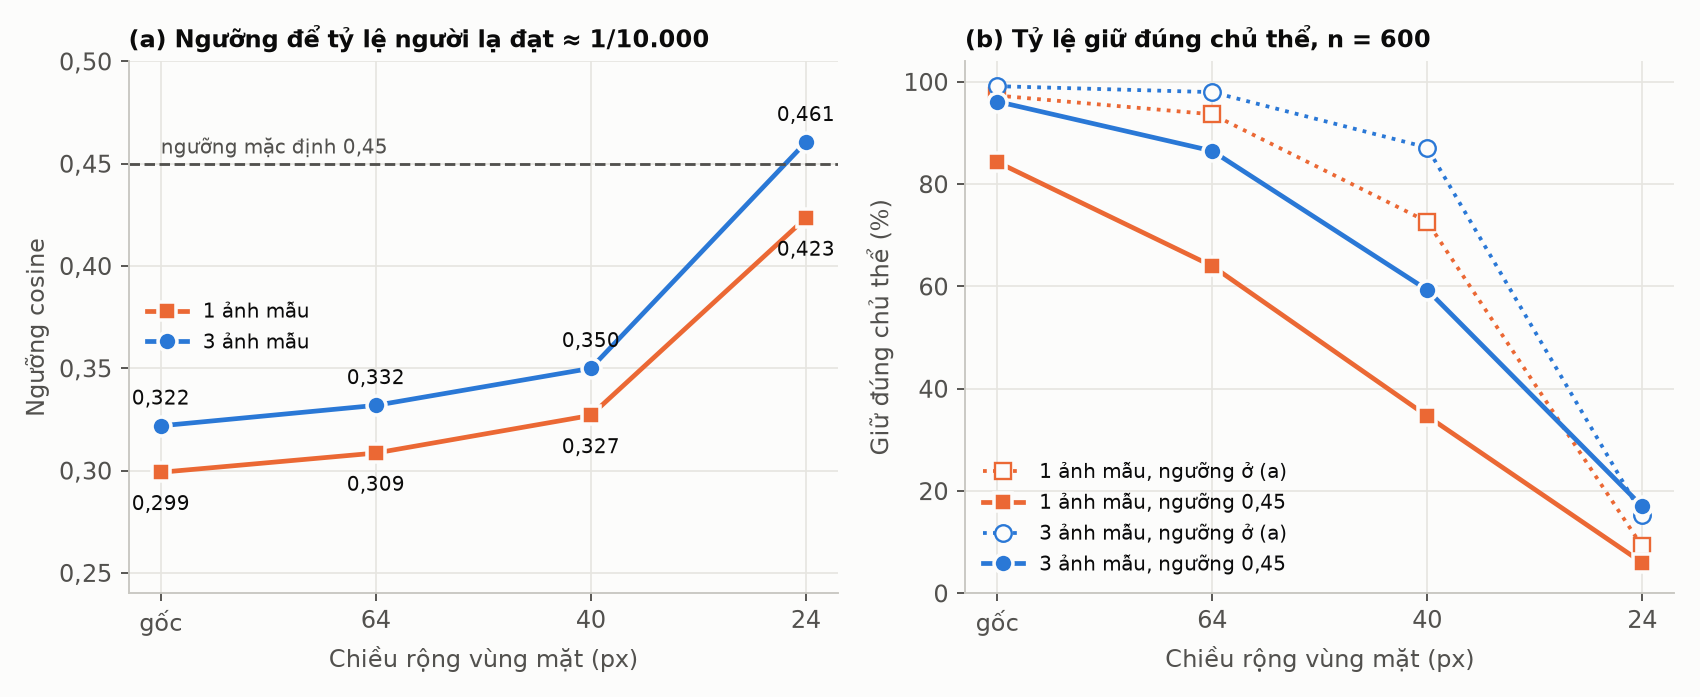
\includegraphics[width=0.98\textwidth]{figures/hinh-4-12-nguong-theo-kich-thuoc.png}
\caption[Ngưỡng similarity theo kích thước khuôn mặt]{Ngưỡng similarity theo kích thước khuôn mặt. (a) Ngưỡng để tỷ lệ người lạ khoảng 1/10.000. (b) TAR tương ứng, so với ngưỡng cố định 0,45}
\label{fig:4-12}
\end{figure}

\textbf{Rủi ro nhận nhầm người lạ.} Với FAR khoảng 3 phần triệu, một video có 1.000 mặt lạ và danh sách 5 người có khoảng 1,7\% khả năng lọt ít nhất một người, nếu coi các phép so là độc lập. Khi lọt, cả đoạn quỹ đạo sẽ không được che, nên nhóm giữ ngưỡng 0,45 thay vì hạ xuống. Nhóm xem lại sáu cặp bị nhận nhầm trên LFW. Bốn cặp đến từ một ảnh có hai người đứng cạnh nhau, hệ thống lấy nhầm mặt của người còn lại. Một cặp dùng ảnh mà danh sách đính chính của LFW ghi là gán sai tên. Chỉ còn một cặp chưa rõ nguyên nhân, nên tỷ lệ nhận nhầm thực tế có thể còn thấp hơn. Trường hợp này cũng cho thấy ảnh mẫu nên chỉ có một khuôn mặt.

\subsection{Đánh giá trên video thực tế}

Đánh giá trên video kiểm tra toàn bộ Engine chứ không chỉ mô hình. Engine chạy trước trên từng clip, kết quả được đưa vào CVAT dưới dạng quỹ đạo để sửa tay và gán danh tính chủ thể hoặc người lạ. Với mỗi hộp nhãn ở mỗi khung, nhóm tính phần diện tích thực sự được che, gồm cả vết nội suy và vết giữ 200 ms. Tỷ lệ bỏ sót là tỷ lệ nhãn không được che chút nào, còn tỷ lệ giữ đúng là số khung của chủ thể được giữ rõ. Bảng~\ref{tab:4-8} so năm thời điểm: trước hai bản sửa Engine, sau hai bản sửa, sau khi sửa danh sách miễn che, và hai mô hình dashcam cuối cùng.

\begin{table}[!htp]
\centering\bangnho
\caption{Kết quả che và whitelist trên clip video (\%)}\label{tab:4-8}
\begin{tabular}{|L{2.1cm}|L{4.7cm}|C{1.3cm}|C{1.4cm}|C{1.5cm}|C{1.5cm}|C{1.2cm}|}
\hline
\dongdau \textbf{Clip} & \textbf{Chỉ số (số nhãn)} & \textbf{Trước sửa} & \textbf{Sau 2 bản sửa} & \textbf{Sửa miễn che} & \textbf{Max privacy} & \textbf{Fast} \\ \hline
Dashcam 1 & Biển bỏ sót (1.668) & 22,8 & 10,6 & 10,6 & \textbf{2,3} & 5,7 \\ \cline{2-7}
 & \quad rộng từ 40 px (1.627) & 21,8 & 9,8 & 9,8 & \textbf{2,3} & 5,3 \\ \cline{2-7}
 & \quad bị che một phần (219) & 55,7 & 30,6 & 30,6 & \textbf{11,9} & 21,5 \\ \cline{2-7}
 & Biển che đủ 90\% (1.668) & 56,9 & 70,4 & 70,4 & 76,6 & 74,6 \\ \cline{2-7}
 & Mặt bỏ sót (481) & 0,0 & 0,0 & 0,0 & 0,0 & 8,9 \\ \cline{2-7}
 & Giữ đúng biển chủ xe (894) & 86,0 & 69,5 & 67,8 & 69,7 & 68,9 \\ \hline
Dashcam 2 & Biển bỏ sót, từ 40 px (64) & 73,4 & 32,8 & 32,8 & \textbf{9,4} & 9,4 \\ \cline{2-7}
 & Mặt bỏ sót (420) & 0,0 & 0,0 & 0,0 & 0,0 & 0,2 \\ \cline{2-7}
 & Giữ đúng biển chủ xe (1.245) & 87,9 & 75,0 & 75,0 & \textbf{89,2} & 83,8 \\ \hline
Điện thoại 1 & Mặt bỏ sót (828) & 1,9 & 0,0 & 0,0 & 0,0 & 0,7 \\ \cline{2-7}
 & Mặt che đủ 70\% & 90,1 & 92,1 & 92,1 & 91,4 & 90,2 \\ \cline{2-7}
 & Giữ đúng chủ thể (347) & 74,4 & 70,3 & 70,3 & 70,3 & 69,5 \\ \hline
Điện thoại 2a & Mặt bỏ sót (1.494) & 5,0 & 0,0 & 0,0 & 0,0 & 0,0 \\ \cline{2-7}
 & Mặt che đủ 70\% & 80,8 & 93,3 & 93,3 & 93,2 & 93,4 \\ \cline{2-7}
 & Giữ đúng chủ thể (549) & 71,2 & 60,1 & 59,4 & 58,3 & 61,6 \\ \hline
Điện thoại 2b & Mặt bỏ sót (1.074) & 4,8 & 0,4 & 0,4 & 0,4 & 2,1 \\ \cline{2-7}
 & Mặt che đủ 70\% & 85,5 & 94,6 & 94,6 & 92,9 & 90,6 \\ \cline{2-7}
 & Giữ đúng chủ thể (699) & 75,5 & 71,2 & 70,2 & 71,1 & 73,0 \\ \hline
Cả 5 clip & Khung người lạ bị giữ như chủ thể (6.031) & 2 & 5 & 5 & 15 & 11 \\ \hline
\end{tabular}
\end{table}

\textbf{Hai bản sửa Engine.} Khi chấm các clip này, nhóm phát hiện hai lỗi của luồng video: bộ lọc theo vị trí bỏ qua mặt người thật, và các phát hiện chưa được ByteTrack xác nhận bị loại trước bước che. Sau khi sửa, mặt bỏ sót ở clip điện thoại giảm từ 1,9--5,0\% xuống 0--0,4\%, biển bỏ sót ở clip dashcam 1 giảm từ 22,8\% xuống 10,6\%. Số đoạn bị lộ từ 200 ms trở lên ở clip này giảm từ 19 xuống 15. Đổi lại, tỷ lệ giữ đúng chủ thể giảm, vì các phát hiện mới tạo thành những đoạn rất ngắn, khó khớp danh sách miễn che nên bị che. Cách sửa được trình bày ở mục 5.3.

\textbf{Biển nhỏ và biển bị che.} Mô hình học từ ảnh cận cảnh nên trước bước 8 còn bỏ sót 9,8\% biển rộng từ 40 px trên clip dashcam 1. Sau khi học thêm khung dashcam, Max privacy chỉ còn 2,3\%, biển bị che một phần giảm từ 30,6\% xuống 11,9\%. Fast giảm từ 11,4\% xuống 5,3\%. Ở clip dashcam 2, Max privacy giảm từ 32,8\% xuống 9,4\%, nhưng clip này chỉ có 64 biển nên mỗi biển ứng với khoảng 1,5 điểm phần trăm. Mặt trái của bước 8 là mô hình nhận logo trắng trên đồng hồ xe của người quay thành biển (1.730 hộp với Max privacy và 269 hộp với Fast), gây che thừa nhưng không lộ thông tin.

\textbf{Giữ đúng chủ thể.} Tính chung, Max privacy giữ đúng 81,1\% khung biển của chủ xe và 66,5\% khung mặt của chủ thể, Fast là 77,6\% và 68,3\%. Việc chuyển sang đọc các vùng cắt rộng nhất giúp hai cấu hình trên clip dashcam 2 tăng từ 34\% lên 82\% và từ 38\% lên 84\%. Số khung người lạ bị giữ nhầm tăng từ 5 lên 15 (Max privacy) và 11 (Fast) trên 6.031 khung, đều nằm ở hai clip dashcam và phần lớn là biển đã được che một phần. Không có khuôn mặt người lạ nào bị giữ nhầm trong ba clip điện thoại.

\textbf{Điểm yếu của Fast.} Trên clip dashcam 1, Fast bỏ sót 8,9\% khung mặt (43/481), còn Max privacy không bỏ sót. Nếu người dùng ưu tiên an toàn cho video hành trình thì nên chọn Max privacy.

\textbf{Lọc mục cần xem lại.} Một video thử dài 18 giây ban đầu có tới 88 mục cần xem lại, quá nhiều để người dùng kiểm tra hết. Trong 260 quỹ đạo của video, 215 quỹ đạo ngắn hơn 0,5 giây và chỉ lệch điểm ở vài khung. Chỉ giữ quỹ đạo từ 0,5 giây còn 34 mục, thêm điều kiện có đoạn điểm thấp hoặc mất dấu từ 0,25 giây thì còn 7 mục. Những mục bị lọc khỏi danh sách vẫn được che bình thường.

\begin{figure}[!htp]
\centering
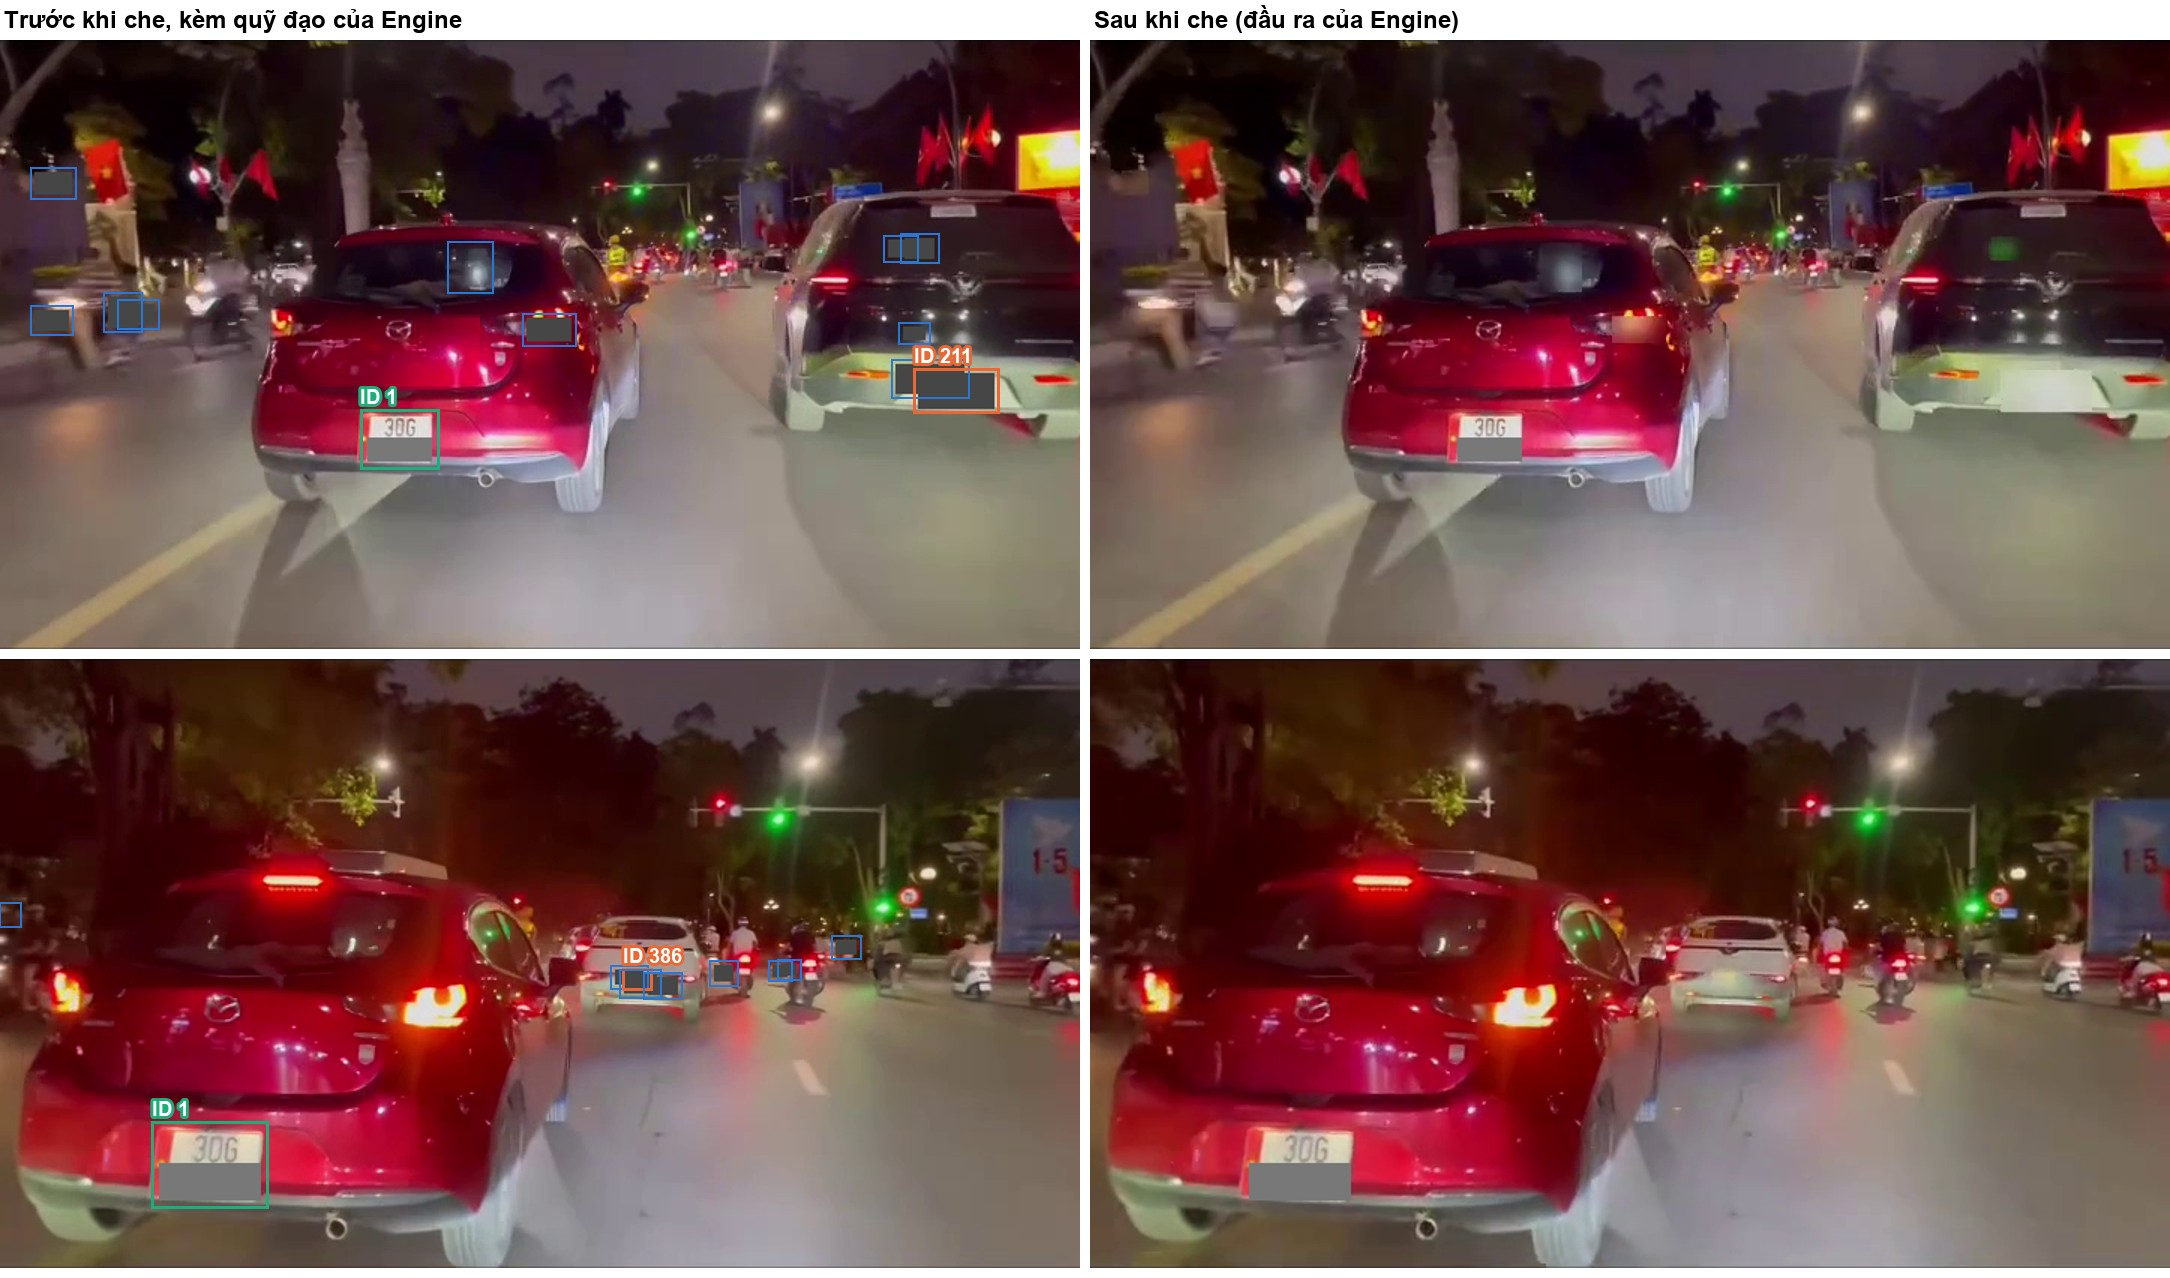
\includegraphics[width=0.98\textwidth]{figures/hinh-4-13-truoc-sau.jpg}
\caption[Ví dụ khung hình video trước và sau khi che]{Hai khung của clip dashcam 2, trước (trái) và sau khi che (phải), chế độ Max privacy. Khung xanh lá là quỹ đạo của chủ xe được giữ rõ, khung cam là phát hiện hiện tại, khung xanh dương là vết che giữ thêm 200 ms. Ô xám được thêm khi in để không lộ biển số}
\label{fig:4-13}
\end{figure}

Hình~\ref{fig:4-13} cho thấy biển của chủ xe được giữ rõ liên tục 234 khung, trong khi biển xe khác bị che. Nhiều vết che nhỏ là báo nhầm ánh đèn và phản chiếu, hệ quả của ngưỡng thấp ở chế độ Max privacy.

\textbf{Giới hạn.} Năm clip đều do nhóm chọn, mỗi clip chỉ một người gán nhãn và đã được dùng để sửa Engine. Một phần trường hợp che chưa đủ có thể do nhãn được CVAT nội suy giữa các khung chính. Vì vậy các tỷ lệ có thể thay đổi vài điểm khi có thêm dữ liệu.

\subsection{Chi phí suy luận trên CPU và GPU}

Bảng~\ref{tab:4-9} ghi thời gian và RAM của từng mô hình. Phần đầu đo trên cùng một máy để so được với nhau, phần sau là kết quả của cả Engine trên hai môi trường triển khai. Các nhóm dòng đo trên máy khác nhau nên không so chéo.

\begin{table}[!htp]
\centering\bangnho
\caption{Thời gian suy luận và RAM của từng mô hình trên CPU và GPU}\label{tab:4-9}
\begin{tabular}{|L{3.0cm}|C{1.7cm}|L{4.3cm}|C{2.7cm}|C{2.8cm}|}
\hline
\dongdau \textbf{Mô hình} & \textbf{Đầu vào} & \textbf{Runtime} & \textbf{Thời gian} & \textbf{RAM đỉnh} \\ \hline
\multicolumn{5}{|l|}{\textit{Từng mô hình, Core Ultra 5 125H giới hạn 4 luồng, chỉ CPU}} \\ \hline
YOLO26n & 960 & PyTorch, 2 luồng & 125 ms/ảnh & 602 MB \\ \hline
YOLO26n & 1280 & PyTorch, 2 luồng & 178 ms/ảnh & 672 MB \\ \hline
YOLO26s & 960 & PyTorch, 2 luồng & 240 ms/ảnh & 741 MB \\ \hline
YOLO26s & 1280 & PyTorch, 2 luồng & 389 ms/ảnh & 878 MB \\ \hline
ArcFace + YuNet & 112 & ONNX Runtime & 11,3 ms/mặt & 146 MB \\ \hline
RapidOCR & vùng biển & ONNX Runtime & 134 ms/biển & 260 MB \\ \hline
\multicolumn{5}{|l|}{\textit{Từng mô hình, máy laptop của nhóm}} \\ \hline
YOLO26n & 1280 & i5-12500H, PyTorch, 2 luồng & 153 ms/ảnh & --- \\ \hline
YOLO26s & 1280 & i5-12500H, PyTorch, 2 luồng & 387 ms/ảnh & --- \\ \hline
deface (CenterFace) & toàn ảnh & i5-12500H, ONNX, 2 luồng & 215 ms/ảnh & --- \\ \hline
YOLO26n & 1280 & RTX 3050, PyTorch & 20,4 ms/khung & --- \\ \hline
ArcFace + YuNet & 112 & ONNX Runtime CPU & 13,4 ms/mặt & --- \\ \hline
RapidOCR & vùng biển & ONNX Runtime CPU & 69,3 ms/biển & --- \\ \hline
\multicolumn{5}{|l|}{\textit{Cả Engine, không có danh sách miễn che}} \\ \hline
Fast & 1280 & RTX 3050, 3 worker & p50 61--65 ms & 1.274--1.337 MiB \\ \hline
Max privacy & 1280 & RTX 3050, 3 worker & p50 102--104 ms & 1.331--1.376 MiB \\ \hline
Fast & 1280 & i5-7200U, 2 worker & p50 0,96--1,20 s & 827--870 MiB \\ \hline
Max privacy & 1280 & i5-7200U, 2 worker & p50 2,85--2,99 s & 962--1.149 MiB \\ \hline
\end{tabular}
\end{table}

\textbf{Kích thước đầu vào và RAM.} Giảm từ 1280 xuống 960 px giúp YOLO26n nhanh hơn khoảng 30\% và YOLO26s nhanh hơn khoảng 38\%, nhưng như Bảng~\ref{tab:4-3}, tỷ lệ mặt được che giảm 6,7 điểm phần trăm, nên nhóm vẫn giữ 1280 px. Một tiến trình chỉ chạy YOLO cần 0,6--0,9 GB RAM, trong đó khoảng 0,33 GB là của Python và PyTorch. Đây là lý do worker chỉ giữ một mô hình YOLO trong bộ nhớ. Trọng số được đóng gói sẵn trong ảnh container nên pod không phải tải mô hình khi khởi động.

\textbf{CPU so với GPU.} Trên GPU, Max privacy chậm hơn Fast khoảng 1,7 lần. Trên máy lab chỉ có CPU, khoảng cách là 3 lần. Như vậy cái giá của chế độ an toàn hơn phụ thuộc nhiều vào phần cứng.

\textbf{Chi phí của danh sách miễn che.} Trên máy có GPU, chỉ YOLO chạy bằng GPU, còn YuNet, ArcFace và RapidOCR chạy trên CPU của worker. Khi thêm một ảnh mẫu khuôn mặt, tốc độ của Fast giảm từ 1.646 xuống 309 ảnh/phút, với danh sách hai biển còn 392 ảnh/phút. Max privacy giảm từ 1.232 xuống 262 và 309 ảnh/phút. Khi có danh sách khuôn mặt, RAM của worker ảnh lên 1.532 MiB, rất sát giới hạn 1.536 MiB.

\textbf{Video.} Nhóm chạy Fast trên đoạn 10 giây (300 khung) của clip dashcam 1 ở ba độ phân giải, YOLO chạy trên RTX 3050. Danh sách miễn che gồm một mặt và một biển không có trong clip, tức trường hợp tốn thời gian nhất:

\begin{center}
\bangfont
\begin{tabular}{|L{3.2cm}|C{2.4cm}|C{2.6cm}|C{3.0cm}|C{3.3cm}|}
\hline
\dongdau \textbf{Độ phân giải} & \textbf{Miễn che} & \textbf{Tốc độ} & \textbf{Thời gian xử lý} & \textbf{Trong đó OCR biển} \\ \hline
854$\times$480 & không & 36,6 fps & 8,2 s & --- \\ \cline{2-5}
 & có & 5,6 fps & 53,6 s & 44,1 s \\ \hline
1280$\times$720 & không & 27,6 fps & 10,9 s & --- \\ \cline{2-5}
 & có & 2,6 fps & 113,7 s & 101,1 s \\ \hline
1920$\times$1080 & không & 15,6 fps & 19,3 s & --- \\ \cline{2-5}
 & có & 2,2 fps & 139,6 s & 119,8 s \\ \hline
\end{tabular}
\end{center}

Ở 1080p, danh sách miễn che làm thời gian tăng từ 19,3 lên 139,6 giây, gần như toàn bộ do OCR biển số. Engine đọc tối đa sáu vùng cắt mỗi quỹ đạo và chỉ dừng sớm khi khớp, trong khi đoạn này có tới 711 quỹ đạo. RAM của tiến trình lên tới 1.968 MB, sát giới hạn 2.048 MiB của worker video, nên nhóm chưa thể khẳng định pod an toàn với video dài hơn.

\subsection{Kết luận chương}

\textbf{Về phát hiện và che.} Từ mô hình có sẵn đến YOLO26s tinh chỉnh ở 1280 px, tỷ lệ mặt đạt tiêu chí che tăng từ 44,9\% lên 79,5\% ở cùng mức precision khoảng 0,78, và lên 83,4\% khi dùng ngưỡng của Max privacy. Kích thước đầu vào ảnh hưởng nhiều hơn cỡ mô hình. Trên video, hai bản sửa Engine đưa mặt bỏ sót trên clip điện thoại xuống 0--0,4\%, còn khung dashcam giảm biển bỏ sót từ 9,8\% xuống 2,3\% (Max privacy) và từ 11,4\% xuống 5,3\% (Fast) với biển rộng từ 40 px.

\textbf{Về danh sách miễn che.} Với khuôn mặt, hệ thống giữ đúng chủ thể 84,3\% khi có một ảnh mẫu và 96,2\% khi có ba ảnh, nhưng giảm mạnh với mặt nhỏ và chỉ đạt 58--73\% trên video điện thoại. Với biển số, bộ so khớp giữ đúng 97,4\% biển cận cảnh và 69--89\% khung biển trong video. Phần lớn sai sót là che nhầm chủ thể, tức sai về phía an toàn.

\textbf{So với mục tiêu ở Chương 1.} Mục tiêu mAP\textsubscript{50} từ 85\% đạt ở trung bình hai lớp (87,0\% và 86,5\%), nhưng riêng lớp mặt mới đạt 77,3\% và 74,8\%. Mục tiêu giữ đúng người quen 85\% đạt khi có ba ảnh mẫu, gần đạt với một ảnh mẫu và chưa đạt trên video.

\textbf{Các điểm còn yếu.} Mặt dưới 16 px mới được che 71,4\% ở Max privacy, vì ở kích thước này gần như không còn chi tiết để nhận ra. Biển bị che một phần vẫn bị bỏ sót 11,9\% do dữ liệu huấn luyện hầu như không có mẫu như vậy. Chế độ Fast còn bỏ sót 8,9\% khung mặt trên một clip dashcam, và có 11--15 khung người lạ bị giữ như chủ thể. Ngoài ra, bộ đánh giá ảnh và các clip đều đã được dùng khi chọn mô hình, nên kết quả cần được kiểm chứng thêm trên dữ liệu mới.



\clearpage
\section{Xây dựng, triển khai và đánh giá}
\label{sec:ch5}

{\small\itshape\noindent\textbf{Ghi chú biên soạn:} Nội dung: Không mô tả lại thiết kế ở Chương 3. Chương này chỉ tập trung vào: những gì thực sự được cài đặt; các vấn đề gặp phải khi triển khai và cách xử lý; những quyết định khác với thiết kế ban đầu; các điểm đáng chú ý trong code.  Nguồn: docs/report-material/decisions.md\par\vspace{6pt}}


\subsection{Backend Web}

{\small\itshape\noindent\textbf{Ghi chú biên soạn:} Nội dung: Những gì đã cài đặt (Express, Prisma, Zod; JWT và refresh token; rate-limit; presigned URL; zip dạng luồng) và các vấn đề gặp phải khi triển khai: tải cả batch trong một multipart bị giới hạn RAM nên đổi sang tải từng file; lifecycle 24 giờ của MinIO xoá file khi dòng DB còn nên chuyển việc xoá về web; xử lý 429 và Retry-After khi tải lên. Điểm đáng chú ý: đồng bộ sự kiện idempotent từ jobs.events.  Nguồn: web/backend/src/, web/README.md\par\vspace{6pt}}

\needspace{8\baselineskip}
{\bangfont
\begin{longtable}{|>{\centering\arraybackslash\bfseries}m{2.13cm}|>{\raggedright\arraybackslash}m{4.37cm}|>{\raggedright\arraybackslash}m{5.82cm}|>{\centering\arraybackslash}m{2.43cm}|}
\caption{Danh sách API chính}\label{tab:5-1}\\
\hline
\dongdau \textbf{Phương thức} & \textbf{Đường dẫn} & \textbf{Chức năng} & \textbf{Xác thực} \\
\hline
\endfirsthead
\multicolumn{4}{c}{\textbf{Bảng 5.1.} Danh sách API chính (tiếp theo)}\\[2pt]
\hline
\dongdau \textbf{Phương thức} & \textbf{Đường dẫn} & \textbf{Chức năng} & \textbf{Xác thực} \\
\hline
\endhead
\endfoot
\endlastfoot
 &  &  & \\ \hline
 &  &  & \\ \hline
\end{longtable}
}
\vspace{6pt}

{\small\itshape\noindent\textbf{Ghi chú biên soạn:} Nhóm theo auth, batches, files/upload, jobs, face-lists, download.  Nguồn: web/backend/src/routes/\par\vspace{6pt}}


\subsection{Frontend Web}

{\small\itshape\noindent\textbf{Ghi chú biên soạn:} Nội dung: Cách triển khai: React, Vite, TypeScript; bản build tĩnh được Express phục vụ trong cùng một image web. Điểm đáng chú ý: xem trước vùng che bằng canvas dùng đúng công thức độ mạnh của Engine.  Nguồn: web/frontend/, web/Dockerfile\par\vspace{6pt}}


\subsection{Engine worker}

Thiết kế của Engine đã trình bày ở mục 3.8. Phần này chỉ nói về những chỗ phải làm khác đi khi cài đặt, vì sao phải đổi và kết quả sau khi đổi. Số liệu chi tiết nằm ở Chương 4.

{\bangfont
\begin{longtable}{|L{4.3cm}|L{4.9cm}|L{5.8cm}|}
\hline
\dongdau \textbf{Vấn đề gặp phải} & \textbf{Cách giải quyết} & \textbf{Kết quả} \\ \hline
\endhead
Mô hình có sẵn bỏ sót nhiều mặt và biển & Thay YOLOv8n bằng YOLO26 tinh chỉnh, chia hai chế độ & Mặt đạt tiêu chí che từ 44,9\% lên 76,7\% (Fast) và 79,5\% (Max privacy) \\ \hline
Bộ lọc theo vị trí bỏ qua mặt người thật & Gỡ bộ lọc & Mặt bỏ sót trên ba clip điện thoại từ 1,9--5,0\% còn 0--0,4\% (đo chung với dòng dưới) \\ \hline
Phát hiện chưa được ByteTrack xác nhận bị mất & Tách YOLO và ByteTrack thành hai bước & Biển bỏ sót trên clip dashcam 1 từ 22,8\% còn 10,6\% (đo chung với dòng trên) \\ \hline
OCR đọc biển lúc còn nhỏ, mờ & Đọc các vùng cắt rộng nhất của quỹ đạo & Hai cấu hình bị ảnh hưởng giữ đúng biển chủ xe từ 34--38\% lên 82--84\% \\ \hline
Một mã quỹ đạo chuyển sang vật khác & Tách quỹ đạo khi mất dấu quá 167 ms & Mỗi đoạn được xét miễn che riêng \\ \hline
Pod phụ thuộc mạng, có thể chạy nhầm mô hình & Đóng gói trọng số vào ảnh container, báo lỗi khi thiếu & Worker không phải tải mô hình khi khởi động \\ \hline
Job treo hoặc quá dài bị chạy lại nhiều lần & Đặt hạn thời gian cho từng loại job & Job quá hạn dừng một lần với lỗi rõ ràng \\ \hline
\end{longtable}\addtocounter{table}{-1}}

\textbf{Thay mô hình phát hiện.} Bản đầu tiên dùng YOLOv8n huấn luyện sẵn trên Open Images, vì mô hình này đã có sẵn lớp mặt người và biển số. Cách làm này giúp nhóm dựng được toàn bộ luồng xử lý sớm, nhưng chất lượng chưa đủ: trên tập đánh giá chỉ 44,9\% số mặt đạt tiêu chí che. Nhóm chuyển sang YOLO26 tinh chỉnh với hai nhãn mặt và biển. Tên lớp của mô hình được ánh xạ về hai nhãn chung nên khi đổi mô hình, phần còn lại không phải sửa. Mỗi chế độ có một chuỗi cấu hình riêng gồm trọng số, kích thước đầu vào và ngưỡng từng lớp. Do RAM của pod có hạn, worker chỉ giữ một mô hình YOLO và đổi khi job sau dùng chế độ khác.

Mô hình mới cũng có điểm trừ. Sau khi học thêm từ khung dashcam, nó nhận nhầm logo trắng trên đồng hồ xe là biển số. Nhóm chấp nhận vì lỗi này chỉ che thừa, không làm lộ thông tin.

\textbf{Bỏ bộ lọc theo vị trí.} Trong video quay từ xe máy, đèn trợ sáng hay bị nhận nhầm là khuôn mặt. Nhóm từng thêm một bộ lọc bỏ các hộp mặt gần vuông ở vùng bên phải phía dưới khung hình. Bộ lọc chạy đúng với video hành trình nhưng lại áp dụng cho mọi video. Với clip quay bằng điện thoại, người thật có thể đứng đúng chỗ đó, và có 83 khung mặt người lạ không được che. Nhóm gỡ hẳn bộ lọc: thà che nhầm một chiếc đèn còn hơn để lộ một khuôn mặt.

\textbf{Giữ lại phát hiện chưa có mã.} Lúc đầu nhóm dùng chức năng theo dõi tích hợp sẵn của Ultralytics. Khi so với cách chạy YOLO trên từng khung, nhóm thấy điều lạ: trên cùng một clip, mô hình tìm được 93,0\% số mặt nhưng sau khi qua Engine chỉ còn 77,2\%. Nguyên nhân là ByteTrack chỉ trả về quỹ đạo đã được xác nhận, nên khung đầu tiên của một vật mới và các hộp không ghép được đều bị bỏ trước khi đến bước che.

Cách sửa là chạy YOLO và ByteTrack riêng. Hộp nào ByteTrack không trả về vẫn được giữ nếu đạt ngưỡng của lớp, được ghép với hộp ở một hoặc hai khung trước khi IoU trên 0,40, nếu không thì cấp mã mới. Cùng với việc gỡ bộ lọc, thay đổi này giảm số mặt bỏ sót trên các clip điện thoại còn 0--0,4\% và giảm hơn một nửa số biển bỏ sót trên clip dashcam 1. Hai thay đổi được đo cùng lúc nên chưa tách được đóng góp của từng phần. Đổi lại, video có thêm nhiều quỹ đạo rất ngắn. Các đoạn này khó khớp danh sách miễn che nên bị che, khiến tỷ lệ giữ đúng biển chủ xe trên clip dashcam 1 giảm từ 86,0\% xuống 69,5\%.

\textbf{Chọn vùng cắt cho OCR.} Trước đây, mỗi quỹ đạo biển số giữ chủ yếu các vùng cắt ở những khung đầu, đúng lúc biển vừa vào hình nên còn nhỏ hoặc bị khuất. Trên clip dashcam 2, một quỹ đạo dài 755 khung của chính chủ xe bị coi là xe lạ vì lý do này. Engine được sửa để giữ năm vùng cắt rộng nhất của cả quỹ đạo. Hai cấu hình bị ảnh hưởng tăng tỷ lệ giữ đúng từ 34\% lên 82\% và từ 38\% lên 84\%, các cấu hình khác gần như không đổi. Nhóm cũng thử đặt chiều rộng tối thiểu 40 px nhưng bỏ, vì chế độ Fast mất 17 điểm phần trăm trong khi OCR vẫn đọc khớp được biển rộng 37 px.

\textbf{Tách quỹ đạo khi mất dấu.} ByteTrack giữ mã của vật bị mất dấu khoảng hai giây và có thể gán lại cho vật khác. Trong một clip, mã của xe lạ chuyển sang xe chủ sau 1,2 giây. Vì quyết định miễn che áp dụng cho cả quỹ đạo, biển xe lạ đã không được che đủ trong khoảng 0,15 giây. Engine hiện mở quỹ đạo mới khi mất dấu quá 167 ms, tức 5 khung ở 30 fps. Mỗi đoạn được xét riêng và khoảng mất dấu được báo cho người dùng. Cách này chưa loại hết rủi ro: một đoạn biển không đọc được chữ vẫn có thể kế thừa quyết định của đoạn nằm cạnh. Trên năm clip, còn 15 khung (Max privacy) và 11 khung (Fast) người lạ bị giữ như chủ thể trong 6.031 khung.

\textbf{Đóng gói trọng số.} Pod có thể được KEDA tạo và thu hồi nhiều lần, hệ thống tệp của container lại ở chế độ chỉ đọc, nên worker không nên tải mô hình lúc khởi động. Toàn bộ trọng số YOLO, ArcFace và YuNet được đưa vào ảnh container. Nhóm cũng tắt tính năng tự cài gói của Ultralytics. Trước đó, khi một video bị gửi nhầm vào hàng đợi ảnh, thư viện này cố cài thêm một gói giải mã HEIC và người dùng nhận được thông báo lỗi chẳng liên quan. Một lỗi khác là khi thiếu tệp trọng số, Engine tự chuyển sang mô hình khác, nên job Max privacy có thể chạy bằng mô hình của Fast mà không ai biết. Engine hiện báo lỗi thay vì tự đổi mô hình.

\textbf{Hạn thời gian cho job.} Worker báo định kỳ cho JetStream rằng job còn đang chạy. Nếu bước suy luận bị treo, tín hiệu này sẽ giữ job ở trạng thái đang xử lý mãi mãi. Lúc đầu nhóm đặt hạn một giờ cho video, quá hạn thì worker thoát và job được giao lại tối đa ba lần. Cách này không hợp với video dài, vì lần sau cũng chậm như lần trước và người dùng chỉ thấy lỗi worker bị sập. Trên máy lab, một clip 33 giây ở 1440p với Max privacy cần khoảng 2--2,5 giờ. Hiện tại hạn là 5 phút với ảnh và 3 giờ với video. Job quá hạn được báo lỗi \code{JOB\_TIMEOUT} đúng một lần.

\textbf{Một số sự cố khác.} Khi chạy thử trên cụm và rà soát lại, nhóm sửa thêm ba trường hợp:
\begin{itemize}
  \item \textit{Kết quả quá lớn.} Một job video dài xử lý xong nhưng sự kiện hoàn tất vượt giới hạn 1 MB của NATS. Worker coi đó là lỗi tạm thời và xử lý lại cả video. Nay worker báo lỗi ngay lần đầu và giới hạn được nâng lên 8 MB. Về lâu dài, phần kết quả chi tiết nên được lưu trên MinIO.
  \item \textit{Lỗi ở một khung.} Trước đây, lỗi phát hiện ở một khung chỉ được ghi log và video vẫn hoàn tất, nghĩa là khung đó có thể không được che. Nay job sẽ báo lỗi, đúng với nguyên tắc ưu tiên riêng tư.
  \item \textit{Tắt worker giữa chừng.} Worker chờ job tối đa 45 giây, nếu chưa xong thì trả job về hàng đợi rồi thoát. Khi thử với NATS thật, worker khác nhận được job ngay, còn bản cũ phải chờ hết thời gian xác nhận là 5 phút.
\end{itemize}

Sau các thay đổi, bộ kiểm thử của Engine gồm 100 ca và đều đạt. Nhóm cũng chạy lại ba đoạn video ngắn trước và sau khi sửa phần xử lý sự cố: kết quả giống hệt nhau, nên số liệu ở Chương 4 không bị ảnh hưởng.

Bài học rút ra là lỗi không chỉ nằm ở mô hình. Bốn vấn đề của luồng video đều nằm ở bước theo dõi hoặc bước xét miễn che, và nhóm chỉ thấy được khi chấm điểm cả Engine trên video có nhãn, thay vì chỉ chấm mô hình trên ảnh.



\subsection{Chính sách lưu trữ, xoá dữ liệu và truyền file}

{\small\itshape\noindent\textbf{Ghi chú biên soạn:} Nội dung: Giữ tới khi người dùng xoá + RETENTION\_DAYS, batch nháp dọn sau 24 giờ, ảnh mẫu whitelist xoá khi batch kết thúc; vì sao bỏ lifecycle 24 giờ của MinIO; presigned URL (1 giờ / 5 phút), token zip 60 giây, tách kết nối nội bộ và công khai. Thư viện media: xoá ảnh hoặc batch là xoá cả object trên MinIO và dòng PostgreSQL. Liên hệ yêu cầu tối thiểu hoá dữ liệu của Luật BVDLCN và GDPR (mục 1.1): ảnh mẫu whitelist là dữ liệu sinh trắc nên được xoá sớm nhất, không bao giờ public.  Nguồn: decisions.md (E, F)\par\vspace{6pt}}

\needspace{8\baselineskip}
{\bangfont
\begin{longtable}{|>{\raggedright\arraybackslash\bfseries}m{2.43cm}|>{\raggedright\arraybackslash}m{4.08cm}|>{\raggedright\arraybackslash}m{4.37cm}|>{\raggedright\arraybackslash}m{3.88cm}|}
\caption{Chính sách lưu giữ theo loại dữ liệu}\label{tab:5-2}\\
\hline
\dongdau \textbf{Loại dữ liệu} & \textbf{Nơi lưu} & \textbf{Thời gian giữ} & \textbf{Cách truy cập} \\
\hline
\endfirsthead
\multicolumn{4}{c}{\textbf{Bảng 5.2.} Chính sách lưu giữ theo loại dữ liệu (tiếp theo)}\\[2pt]
\hline
\dongdau \textbf{Loại dữ liệu} & \textbf{Nơi lưu} & \textbf{Thời gian giữ} & \textbf{Cách truy cập} \\
\hline
\endhead
\endfoot
\endlastfoot
 &  &  & \\ \hline
 &  &  & \\ \hline
\end{longtable}
}
\vspace{6pt}

{\small\itshape\noindent\textbf{Ghi chú biên soạn:} Nguồn: decisions.md (E)\par\vspace{6pt}}


\subsection{Hạ tầng và triển khai}

{\small\itshape\noindent\textbf{Ghi chú biên soạn:} Nội dung: Tenant trên cụm Lab-sock (k3s, node home-server); Kustomize + Helm; NATS, PostgreSQL (Bitnami, pin digest), MinIO tự build; Job setup stream/bucket; SealedSecrets; init container chown; một môi trường imgproc; ghim image engine theo SHA; docker-compose cho dev local; cách cài đặt: chạy toàn bộ hệ thống bằng Docker Compose (profile app) hoặc triển khai lên cụm bằng infra/deploy.sh, kèm các biến môi trường chính.  Nguồn: infra/, decisions.md (G.1-G.13)\par\vspace{6pt}}

\needspace{8\baselineskip}
{\bangfont
\begin{longtable}{|>{\raggedright\arraybackslash\bfseries}m{2.43cm}|>{\raggedright\arraybackslash}m{4.08cm}|>{\raggedright\arraybackslash}m{4.37cm}|>{\raggedright\arraybackslash}m{3.88cm}|}
\caption{Ngân sách tài nguyên các thành phần trên node 2C/4T/12 GB}\label{tab:5-3}\\
\hline
\dongdau \textbf{Thành phần} & \textbf{CPU request/limit} & \textbf{RAM request/limit} & \textbf{Ghi chú} \\
\hline
\endfirsthead
\multicolumn{4}{c}{\textbf{Bảng 5.3.} Ngân sách tài nguyên các thành phần trên node 2C/4T/12 GB (tiếp theo)}\\[2pt]
\hline
\dongdau \textbf{Thành phần} & \textbf{CPU request/limit} & \textbf{RAM request/limit} & \textbf{Ghi chú} \\
\hline
\endhead
\endfoot
\endlastfoot
 &  &  & \\ \hline
 &  &  & \\ \hline
\end{longtable}
}
\vspace{6pt}

{\small\itshape\noindent\textbf{Ghi chú biên soạn:} Tổng nền $\le$ 2.560 Mi, worker báo cáo riêng.  Nguồn: infra/app/*, decisions.md (G.6)\par\vspace{6pt}}

\needspace{8\baselineskip}
{\bangfont
\begin{longtable}{|>{\raggedright\arraybackslash\bfseries}m{3.01cm}|>{\raggedright\arraybackslash}m{2.81cm}|>{\raggedright\arraybackslash}m{2.81cm}|>{\raggedright\arraybackslash}m{2.81cm}|>{\raggedright\arraybackslash}m{3.01cm}|}
\caption{Cấu hình KEDA cho các pool worker}\label{tab:5-4}\\
\hline
\dongdau \textbf{Pool} & \textbf{Trigger} & \textbf{lagThreshold} & \textbf{min/max replica} & \textbf{cooldown} \\
\hline
\endfirsthead
\multicolumn{5}{c}{\textbf{Bảng 5.4.} Cấu hình KEDA cho các pool worker (tiếp theo)}\\[2pt]
\hline
\dongdau \textbf{Pool} & \textbf{Trigger} & \textbf{lagThreshold} & \textbf{min/max replica} & \textbf{cooldown} \\
\hline
\endhead
\endfoot
\endlastfoot
image-worker & nats-jetstream &  &  & \\ \hline
video-worker & nats-jetstream &  &  & \\ \hline
\end{longtable}
}
\vspace{6pt}

{\small\itshape\noindent\textbf{Ghi chú biên soạn:} Nguồn: infra/app/engine-workers/\par\vspace{6pt}}


\begin{figure}[htbp]
\centering
\fbox{\parbox{0.92\textwidth}{\centering\small\itshape [HÌNH 5.1]Ảnh chụp kubectl get pods -n imgproc khi đang xử lý (worker đã scale).}}
\caption{Danh sách pod trong namespace imgproc}
\label{fig:5-1}
\end{figure}


\begin{figure}[htbp]
\centering
\fbox{\parbox{0.92\textwidth}{\centering\small\itshape [HÌNH 5.2]Commit lên main $\rightarrow$ ci.yml (lint/test) $\rightarrow$ images.yml (build và push imgproc-web, imgproc-engine theo SHA) $\rightarrow$ cập nhật kustomization $\rightarrow$ deploy.sh.Nguồn: .github/workflows/ci.yml, images.yml}}
\caption{Quy trình CI/CD với GitHub Actions}
\label{fig:5-2}
\end{figure}


\subsection{Kiểm thử}


\subsubsection{Kiểm thử tự động}

{\small\itshape\noindent\textbf{Ghi chú biên soạn:} Nội dung: Backend và frontend dùng Vitest (frontend kiểm thử theo hành vi), Engine dùng pytest; CI chạy trên mỗi commit; script verify-render và smoke test của hạ tầng.  Nguồn: web/backend/tests, web/frontend/tests, engine/tests, .github/workflows/ci.yml\par\vspace{6pt}}

\needspace{10\baselineskip}
{\bangfont
\begin{longtable}{|>{\raggedright\arraybackslash\bfseries}m{3.01cm}|>{\raggedright\arraybackslash}m{2.81cm}|>{\raggedright\arraybackslash}m{2.81cm}|>{\raggedright\arraybackslash}m{2.81cm}|>{\raggedright\arraybackslash}m{3.01cm}|}
\caption{Tổng hợp kiểm thử tự động}\label{tab:5-5}\\
\hline
\dongdau \textbf{Khối} & \textbf{Công cụ} & \textbf{Số test} & \textbf{Phạm vi} & \textbf{Kết quả} \\
\hline
\endfirsthead
\multicolumn{5}{c}{\textbf{Bảng 5.5.} Tổng hợp kiểm thử tự động (tiếp theo)}\\[2pt]
\hline
\dongdau \textbf{Khối} & \textbf{Công cụ} & \textbf{Số test} & \textbf{Phạm vi} & \textbf{Kết quả} \\
\hline
\endhead
\endfoot
\endlastfoot
Web backend & Vitest &  &  & \\ \hline
Web frontend & Vitest + Testing Library &  &  & \\ \hline
Engine & pytest &  &  & \\ \hline
Infra & verify-render / smoke test &  &  & \\ \hline
\end{longtable}
}
\vspace{6pt}


\subsubsection{Kiểm thử chức năng}

{\small\itshape\noindent\textbf{Ghi chú biên soạn:} Nội dung: Kịch bản kiểm thử thủ công trên môi trường imgproc cho từng nhóm chức năng.\par\vspace{6pt}}

\needspace{13\baselineskip}
{\bangfont
\begin{longtable}{|>{\centering\arraybackslash}m{0.96cm}|>{\raggedright\arraybackslash\bfseries}m{3.37cm}|>{\raggedright\arraybackslash}m{3.37cm}|>{\raggedright\arraybackslash}m{3.37cm}|>{\raggedright\arraybackslash}m{3.37cm}|}
\caption{Kiểm thử chức năng end-to-end}\label{tab:5-6}\\
\hline
\dongdau \textbf{STT} & \textbf{Kịch bản} & \textbf{Dữ liệu vào} & \textbf{Kết quả mong đợi} & \textbf{Kết quả thực tế} \\
\hline
\endfirsthead
\multicolumn{5}{c}{\textbf{Bảng 5.6.} Kiểm thử chức năng end-to-end (tiếp theo)}\\[2pt]
\hline
\dongdau \textbf{STT} & \textbf{Kịch bản} & \textbf{Dữ liệu vào} & \textbf{Kết quả mong đợi} & \textbf{Kết quả thực tế} \\
\hline
\endhead
\endfoot
\endlastfoot
1 & Tài khoản: đăng ký bằng mã, đăng nhập, đổi mật khẩu &  &  & \\ \hline
2 & Tải lên: ảnh, thư mục, video &  &  & \\ \hline
3 & Xử lý: theo dõi tiến độ, thử lại ảnh lỗi &  &  & \\ \hline
4 & Whitelist khuôn mặt và biển số &  &  & \\ \hline
5 & Sửa ảnh và render lại &  &  & \\ \hline
6 & Tải file: từng ảnh, video, zip cả batch &  &  & \\ \hline
7 & Xoá dữ liệu: ảnh, batch, danh sách khuôn mặt &  &  & \\ \hline
\end{longtable}
}
\vspace{6pt}


\subsection{Hiệu năng}


\subsubsection{Thông lượng và khả năng co giãn}

{\small\itshape\noindent\textbf{Ghi chú biên soạn:} Nội dung: Ba chế độ: cố định N worker, autoscale 0$\rightarrow$3, autoscale 1$\rightarrow$3; trên máy có GPU (3.726 ảnh) và máy chỉ có CPU (100 ảnh); thời gian khởi động nguội; web là nút thắt khi giới hạn CPU thấp; 0 job lỗi.  Nguồn: infra/bench/README.md, infra/bench/results/comparison.md\par\vspace{6pt}}

\needspace{8\baselineskip}
{\bangfont
\begin{longtable}{|>{\raggedright\arraybackslash\bfseries}m{2.09cm}|>{\raggedright\arraybackslash}m{1.71cm}|>{\raggedright\arraybackslash}m{2.09cm}|>{\raggedright\arraybackslash}m{2.09cm}|>{\raggedright\arraybackslash}m{2.09cm}|>{\raggedright\arraybackslash}m{2.09cm}|>{\raggedright\arraybackslash}m{1.71cm}|}
\caption{Thông lượng trên máy có GPU (3.726 ảnh)}\label{tab:5-7}\\
\hline
\dongdau \textbf{Mô hình} & \textbf{Đầu vào} & \textbf{Drain, 3 worker} & \textbf{End-to-end, 3 worker} & \textbf{Autoscale 0$\rightarrow$3} & \textbf{Autoscale 1$\rightarrow$3} & \textbf{p50 / ảnh} \\
\hline
\endfirsthead
\multicolumn{7}{c}{\textbf{Bảng 5.7.} Thông lượng trên máy có GPU (3.726 ảnh) (tiếp theo)}\\[2pt]
\hline
\dongdau \textbf{Mô hình} & \textbf{Đầu vào} & \textbf{Drain, 3 worker} & \textbf{End-to-end, 3 worker} & \textbf{Autoscale 0$\rightarrow$3} & \textbf{Autoscale 1$\rightarrow$3} & \textbf{p50 / ảnh} \\
\hline
\endhead
\endfoot
\endlastfoot
 &  &  &  &  &  & \\ \hline
 &  &  &  &  &  & \\ \hline
\end{longtable}
}
\vspace{6pt}

{\small\itshape\noindent\textbf{Ghi chú biên soạn:} Nguồn: infra/bench/results/comparison.md (Final comparison)\par\vspace{6pt}}

\needspace{8\baselineskip}
{\bangfont
\begin{longtable}{|>{\raggedright\arraybackslash\bfseries}m{2.46cm}|>{\raggedright\arraybackslash}m{2.26cm}|>{\raggedright\arraybackslash}m{2.26cm}|>{\raggedright\arraybackslash}m{2.26cm}|>{\raggedright\arraybackslash}m{2.26cm}|>{\raggedright\arraybackslash}m{2.65cm}|}
\caption{Thông lượng trên máy chỉ có CPU (100 ảnh)}\label{tab:5-8}\\
\hline
\dongdau \textbf{Mô hình} & \textbf{Đầu vào} & \textbf{Drain, 2 worker} & \textbf{End-to-end, 2 worker} & \textbf{Autoscale 0$\rightarrow$3} & \textbf{p50 / ảnh} \\
\hline
\endfirsthead
\multicolumn{6}{c}{\textbf{Bảng 5.8.} Thông lượng trên máy chỉ có CPU (100 ảnh) (tiếp theo)}\\[2pt]
\hline
\dongdau \textbf{Mô hình} & \textbf{Đầu vào} & \textbf{Drain, 2 worker} & \textbf{End-to-end, 2 worker} & \textbf{Autoscale 0$\rightarrow$3} & \textbf{p50 / ảnh} \\
\hline
\endhead
\endfoot
\endlastfoot
 &  &  &  &  & \\ \hline
 &  &  &  &  & \\ \hline
\end{longtable}
}
\vspace{6pt}

{\small\itshape\noindent\textbf{Ghi chú biên soạn:} Nguồn: infra/bench/results/comparison.md\par\vspace{6pt}}


\begin{figure}[htbp]
\centering
\fbox{\parbox{0.92\textwidth}{\centering\small\itshape [HÌNH 5.3]Biểu đồ đường từ replicas.csv: số pod và số job chờ theo thời gian (0$\rightarrow$3$\rightarrow$0).Nguồn: infra/bench/results/<máy>/<model>/<size>/<run>/replicas.csv}}
\caption{Số replica worker theo thời gian khi KEDA co giãn}
\label{fig:5-3}
\end{figure}


\begin{figure}[htbp]
\centering
\fbox{\parbox{0.92\textwidth}{\centering\small\itshape [HÌNH 5.4]Biểu đồ cột img/phút cho cố định / 0$\rightarrow$3 / 1$\rightarrow$3.Nguồn: infra/bench/results/comparison.md}}
\caption{So sánh thông lượng giữa các chế độ triển khai}
\label{fig:5-4}
\end{figure}


\begin{figure}[htbp]
\centering
\fbox{\parbox{0.92\textwidth}{\centering\small\itshape [HÌNH 5.5]Biểu đồ mục ``How web is a bottleneck''.Nguồn: infra/bench/results/comparison.md}}
\caption{Ảnh hưởng của giới hạn CPU của web lên thông lượng}
\label{fig:5-5}
\end{figure}


\subsubsection{Hiệu năng xử lý video trên CPU}

{\small\itshape\noindent\textbf{Ghi chú biên soạn:} Nội dung: Thời gian từng công đoạn (decode, detect, track, embed/OCR, redact, encode), hiệu quả whitelist theo track (giảm 99,94\% lượt gọi model), thời gian toàn trình theo độ phân giải, RAM so với giới hạn pod.  Nguồn: engine/docs/benchmark\_cpu\_results.md\par\vspace{6pt}}

\needspace{8\baselineskip}
{\bangfont
\begin{longtable}{|>{\raggedright\arraybackslash\bfseries}m{2.43cm}|>{\raggedright\arraybackslash}m{4.08cm}|>{\raggedright\arraybackslash}m{4.37cm}|>{\raggedright\arraybackslash}m{3.88cm}|}
\caption{Thời gian từng công đoạn xử lý video}\label{tab:5-9}\\
\hline
\dongdau \textbf{Công đoạn} & \textbf{Thời gian} & \textbf{Tỉ lệ} & \textbf{Ghi chú} \\
\hline
\endfirsthead
\multicolumn{4}{c}{\textbf{Bảng 5.9.} Thời gian từng công đoạn xử lý video (tiếp theo)}\\[2pt]
\hline
\dongdau \textbf{Công đoạn} & \textbf{Thời gian} & \textbf{Tỉ lệ} & \textbf{Ghi chú} \\
\hline
\endhead
\endfoot
\endlastfoot
 &  &  & \\ \hline
 &  &  & \\ \hline
\end{longtable}
}
\vspace{6pt}

{\small\itshape\noindent\textbf{Ghi chú biên soạn:} Nguồn: engine/docs/benchmark\_cpu\_results.md §2\par\vspace{6pt}}

\needspace{8\baselineskip}
{\bangfont
\begin{longtable}{|>{\raggedright\arraybackslash\bfseries}m{2.43cm}|>{\raggedright\arraybackslash}m{4.08cm}|>{\raggedright\arraybackslash}m{4.37cm}|>{\raggedright\arraybackslash}m{3.88cm}|}
\caption{Hiệu năng toàn trình theo độ phân giải video}\label{tab:5-10}\\
\hline
\dongdau \textbf{Độ phân giải} & \textbf{Thời lượng clip} & \textbf{Thời gian xử lý} & \textbf{RAM đỉnh} \\
\hline
\endfirsthead
\multicolumn{4}{c}{\textbf{Bảng 5.10.} Hiệu năng toàn trình theo độ phân giải video (tiếp theo)}\\[2pt]
\hline
\dongdau \textbf{Độ phân giải} & \textbf{Thời lượng clip} & \textbf{Thời gian xử lý} & \textbf{RAM đỉnh} \\
\hline
\endhead
\endfoot
\endlastfoot
 &  &  & \\ \hline
 &  &  & \\ \hline
\end{longtable}
}
\vspace{6pt}

{\small\itshape\noindent\textbf{Ghi chú biên soạn:} Nguồn: engine/docs/benchmark\_cpu\_results.md §4\par\vspace{6pt}}


\subsection{Giao diện hệ thống}

{\small\itshape\noindent\textbf{Ghi chú biên soạn:} Nội dung: Ảnh chụp màn hình các trang chính, chú thích ngắn chức năng.\par\vspace{6pt}}


\begin{figure}[htbp]
\centering
\fbox{\parbox{0.92\textwidth}{\centering\small\itshape [HÌNH 5.6]Ảnh chụp màn hình tại https://imgproc.sock1000kg.io.vn.}}
\caption{Giao diện trang tạo batch: tải lên, cấu hình che, whitelist và ảnh xem trước}
\label{fig:5-6}
\end{figure}


\begin{figure}[htbp]
\centering
\fbox{\parbox{0.92\textwidth}{\centering\small\itshape [HÌNH 5.7]Ảnh chụp màn hình tại https://imgproc.sock1000kg.io.vn.}}
\caption{Giao diện xem kết quả ảnh: thanh trượt before/after và báo cáo cần xem lại}
\label{fig:5-7}
\end{figure}


\begin{figure}[htbp]
\centering
\fbox{\parbox{0.92\textwidth}{\centering\small\itshape [HÌNH 5.8]Ảnh chụp màn hình tại https://imgproc.sock1000kg.io.vn.}}
\caption{Giao diện trình xem video kết quả và danh sách cần xem lại}
\label{fig:5-8}
\end{figure}


\begin{figure}[htbp]
\centering
\fbox{\parbox{0.92\textwidth}{\centering\small\itshape [HÌNH 5.9]Ảnh chụp màn hình tại https://imgproc.sock1000kg.io.vn.}}
\caption{Giao diện công cụ Sửa ảnh}
\label{fig:5-9}
\end{figure}


\subsection{Đánh giá mức độ giải quyết}

{\small\itshape\noindent\textbf{Ghi chú biên soạn:} Nội dung: Bảng tổng hợp đối chiếu từng mục tiêu ở Chương 1 với kết quả thực tế; nêu rõ phần đã triển khai, phần đạt một phần, phần chưa làm (kèm lý do).\par\vspace{6pt}}

\needspace{8\baselineskip}
{\bangfont
\begin{longtable}{|>{\raggedright\arraybackslash\bfseries}m{3.01cm}|>{\raggedright\arraybackslash}m{2.81cm}|>{\raggedright\arraybackslash}m{2.81cm}|>{\raggedright\arraybackslash}m{2.81cm}|>{\raggedright\arraybackslash}m{3.01cm}|}
\caption{Tổng hợp mức độ giải quyết so với mục tiêu}\label{tab:5-11}\\
\hline
\dongdau \textbf{Mục tiêu} & \textbf{Đã triển khai} & \textbf{Kết quả đo được} & \textbf{Mức độ (Đạt / Một phần / Chưa)} & \textbf{Nhận xét} \\
\hline
\endfirsthead
\multicolumn{5}{c}{\textbf{Bảng 5.11.} Tổng hợp mức độ giải quyết so với mục tiêu (tiếp theo)}\\[2pt]
\hline
\dongdau \textbf{Mục tiêu} & \textbf{Đã triển khai} & \textbf{Kết quả đo được} & \textbf{Mức độ (Đạt / Một phần / Chưa)} & \textbf{Nhận xét} \\
\hline
\endhead
\endfoot
\endlastfoot
 &  &  &  & \\ \hline
 &  &  &  & \\ \hline
\end{longtable}
}
\vspace{6pt}

{\small\itshape\noindent\textbf{Ghi chú biên soạn:} Gồm cả mục tiêu chức năng (ảnh, video, whitelist, tài khoản\dots{}) và mục tiêu định lượng (AI, hệ thống).  Nguồn: docs/milestones.md, web/docs/plan.md, engine/docs/plan.md\par\vspace{6pt}}


\clearpage
\section*{Kết luận}
\addcontentsline{toc}{section}{Kết luận}


\subsection*{Kết quả đạt được}
\addcontentsline{toc}{subsection}{Kết quả đạt được}

{\small\itshape\noindent\textbf{Ghi chú biên soạn:} Nội dung: Tóm tắt những gì đã xây dựng ở ba khối Web, Engine/AI, Infra và các con số chính.\par\vspace{6pt}}


\subsection*{Hạn chế}
\addcontentsline{toc}{subsection}{Hạn chế}

{\small\itshape\noindent\textbf{Ghi chú biên soạn:} Nội dung: Ví dụ: chưa có benchmark video có nhãn đầy đủ; dữ liệu biển số cận cảnh khác dashcam; RETENTION\_DAYS toàn hệ thống; chạy trên một node; sửa kết quả mới có cho ảnh, chưa có cho video.\par\vspace{6pt}}


\subsection*{Hướng phát triển}
\addcontentsline{toc}{subsection}{Hướng phát triển}

{\small\itshape\noindent\textbf{Ghi chú biên soạn:} Nội dung: Ví dụ: dữ liệu biển số dashcam và mặt rất nhỏ, thời hạn lưu theo người dùng, mở rộng nhiều node / GPU, thêm lớp đối tượng (màn hình, giấy tờ), tích hợp API cho bên thứ ba.\par\vspace{6pt}}


\subsection*{Kiến thức và kỹ năng đạt được}
\addcontentsline{toc}{subsection}{Kiến thức và kỹ năng đạt được}

{\small\itshape\noindent\textbf{Ghi chú biên soạn:} Nội dung: Bài học về làm việc nhóm qua hợp đồng tích hợp chung, huấn luyện và đánh giá mô hình có phương pháp, vận hành Kubernetes trên tài nguyên hạn chế.\par\vspace{6pt}}


\clearpage
\section*{Tài liệu tham khảo}
\addcontentsline{toc}{section}{Tài liệu tham khảo}

{\small\itshape\noindent\textbf{Ghi chú biên soạn:} Nội dung: Trích dẫn theo một chuẩn thống nhất (IEEE hoặc APA). Dự kiến gồm:\par\vspace{6pt}}

{\small\itshape\noindent\textbf{Ghi chú biên soạn:} Văn bản pháp lý: Luật BVDLCN 91/2025/QH15; Nghị định 356/2025/NĐ-CP; GDPR (EU 2016/679).\par\vspace{6pt}}

{\small\itshape\noindent\textbf{Ghi chú biên soạn:} Bài báo / mô hình: YOLO (Ultralytics YOLOv8, YOLO11, YOLO26), WIDER FACE, ArcFace, YuNet, ByteTrack, PP-OCR, CenterFace/deface, EgoBlur, LFW.\par\vspace{6pt}}

{\small\itshape\noindent\textbf{Ghi chú biên soạn:} Tài liệu công nghệ: NATS JetStream, KEDA, Kubernetes, MinIO, PostgreSQL, Prisma, React, Express, FFmpeg, ONNX Runtime.\par\vspace{6pt}}

{\small\itshape\noindent\textbf{Ghi chú biên soạn:} Bộ dữ liệu biển số Việt Nam đã dùng (ghi rõ nguồn và giấy phép).\par\vspace{6pt}}

\end{document}
